%Empieza configuracion de capitulo
\setstretch{1.0}
\titleformat{\chapter}[block]{\Large\bfseries}{CHAPTER \Huge\thechapter\vspace{25 pt}}{0 pt}{\\\fontsize{26}{36}\selectfont}
\titlespacing{\chapter}{0 pt}{30 pt}{50 pt}[0 pt]
\titleformat{\section}{\Large\bfseries}{\thesection}{0 pt}{\hspace{30 pt}}
\titleformat{\subsection}{\large\bfseries}{\thesubsection}{0 pt}{\hspace{30 pt}}
\pagestyle{fancy}
\fancyhead[LO,LE]{\footnotesize\emph{\leftmark}}
\fancyhead[RO,RE]{\thepage}
\fancyfoot[CO,CE]{}
%Termina configuracion de capitulo

\chapter{Experiments and Results}
\setstretch{1.5} %Regresa el interlineado a 1.5

\normalsize
\noindent

This section describes the experiments and results while searching to 
conditions for the embedded distributed system. Each experiment is described 
in the same order it was tested and explained the reasons why that it was run.
The steps that are involved are: 

\begin{itemize}
\item To run a simple sanity test in the embedded platform.
\item To run the MPI Bench test suite in the embedded platform.
\item To evaluate operating systems for the embedded platform.
\item To evaluate MPI library.
\item To test MPI in a cluster of embedded systems.
\item To compare the performance between a cluster of embedded systems to a
traditional computing system, using MPI bench.
\item To compare the power consumption of a cluster of embedded systems to a
traditional computing system, using MPI bench.
\end{itemize}

\section{MPI Sanity Testing in an Embedded Platform}

The system under test (Hardware and Software) for this experiment is described
in the Table~\ref{tab:mpi_sanity}

    \begin{center}
    \begin{tabular}{ | l | r |}
        \hline
        \textbf{Platform under test} &  MinnowBoard MAX \\ \hline
        \textbf{Number of platforms}  & 1  \\ \hline
        \textbf{Operating System} & Fedora  \\ \hline
    \end{tabular}
    \captionof{table}{Description of system under test (HW/SW) for MPI sanity testing
    experiment}\label{tab:mpi_sanity}
    \end{center}

To find the environment that gives better performance of  MPIbench tests, first
it is necessary to run the basic and simple MPI test. A simple code to prove
that the MPI implementation is working as expected is shown in
Figure~\ref{mpi_helloworld}


\begin{minipage}{\textwidth}
\end{minipage}

\begin{minipage}{\textwidth}
\begin{lstlisting}[frame=single,numbers=left,breaklines=true,language=C]
/*************************************************************************
* AUTHOR: Blaise Barney
* https://computing.llnl.gov/tutorials/mpi/samples/C/mpi_hello.c
**************************************************************************/
#include "mpi.h"
#include <stdio.h>
#include <stdlib.h>
#define  MASTER     0

int main (int argc, char *argv[]){
    int   numtasks, taskid, len;
    char hostname[MPI_MAX_PROCESSOR_NAME];

    // Initialize the MPI environment
    MPI_Init(&argc, &argv);
    MPI_Comm_size(MPI_COMM_WORLD, &numtasks);

    // Get the rank of the process
    MPI_Comm_rank(MPI_COMM_WORLD,&taskid);

    // Get the name of the processor
    MPI_Get_processor_name(hostname, &len);

    // Print off a hello world message
    printf ("Hello from task % d on % s!\n", taskid, hostname);
    if (taskid == MASTER)
           printf("MASTER: Number of MPI tasks is: % d\n",numtasks);
    
    // Finalize the MPI environment.
    MPI_Finalize();
}
\end{lstlisting}
\captionof{figure}{MPI code in C to print taskid, hostname and number of MPI tasks}
\label{mpi_helloworld} 
\end{minipage}

\newpage

The way to compile it is: 

\begin{minipage}{\textwidth}
\end{minipage}

\begin{minipage}{\textwidth}
\begin{lstlisting}[frame=single]
  $ mpicc -o mpi_hello_world mpi_hello_world.c
\end{lstlisting}
\end{minipage}

The way to run it is: 

\begin{minipage}{\textwidth}
\end{minipage}

\begin{minipage}{\textwidth}
\begin{lstlisting}[frame=single]
  $ mpirun -n 4 -f host_file ./mpi_hello_world
\end{lstlisting}
\end{minipage}

The program is compiled, it is ready to be executed. Running MPI programs on a
cluster of nodes requires to setup a host file

The host file contains names of all of the compute nodes on which the  MPI job will
execute. For ease of execution, all of the nodes must have SSH access, and should 
have an \textit{authorized keys} file to avoid password prompts for SSH. A
simple host file looks like the one shown in Figure~\ref{hostfile}.

\begin{minipage}{\textwidth}
\end{minipage}

\begin{minipage}{\textwidth}
\begin{lstlisting}[frame=single]
  $ cat hostfile
    node1
    node2
    node3
\end{lstlisting}
\captionof{figure}{MPI hostfile example}
\label{hostfile}
\end{minipage}

Each of the nodes is described in a ssh file as the one shown in
Figure~\ref{ssh_config}.

\begin{minipage}{\textwidth}
\end{minipage}

\begin{minipage}{\textwidth}

\begin{lstlisting}[frame=single]
  $ cat ~/.ssh/config
    Host node1
        HostName node1-ip-or-hostname
        User user-of-the-ssh-key
        Port port-if-nedded
\end{lstlisting}
\captionof{figure}{ssh configuration file example}
\label{ssh_config}
\end{minipage}

To run on a single system is not necessary to have a host file; however, for
the experiments of this work it was needed more than one system.

The result of the basic MPI test is shown in Figure~\ref{mpi_sanity_run}

\begin{minipage}{\textwidth}
\end{minipage}

\begin{minipage}{\textwidth}
\begin{lstlisting}[frame=single]
victor@minnow-1 tmp $ mpirun -n 4  ./hello
Hello from task 0 on minnow-1
MASTER: Number of MPI tasks is: 4
Hello from task 1 on minnow-1
Hello from task 2 on minnow-1
Hello from task 3 on minnow-1
\end{lstlisting}
\captionof{figure}{Results of MPI basic code in Figure~\ref{mpi_helloworld}}
\label{mpi_sanity_run}
\end{minipage}

\subsection{Results}

After this experiment completed in the embedded platform with a regular GNU/Linux
OS (Fedora), It was proved that it is possible to run MPI in an embedded
system. However, there are different GNU/Linux Operating Systems
(for example, Suse/Debian/RedHat). Next is needed to evaluate whether exists a
Linux based operating system for embedded systems which would provide the best
power efficiency. 

\section{Evaluation of MPI Benchmarks Testing in an Embedded Platform}
    
The system under test (Hardware and Software) for this experiment is described
in the Table~\ref{tab:mpi_mpibench}

    \begin{center}
    \begin{tabular}{ | l | r |}
        \hline
        \textbf{Platform under test} &  MinnowBoard MAX \\ \hline
        \textbf{Number of platforms}  & 1  \\ \hline
        \textbf{Operating System} & Fedora  \\ \hline
    \end{tabular}
    \captionof{table}{Description of system under test (HW/SW) for MPI
    benchmarks experiment}\label{tab:mpi_mpibench}
    \end{center}

The first approach is  to find if it is possible to run a sanity MPI test
(Figure~\ref{mpi_helloworld}) with a regular GNU Linux operating system on the embedded
system (MinnowBoard MAX \cite{minnowboard}),  From the list of GNU/Linux
based operating systems that support the embedded system \cite{minnowboard}
the one we selected was Fedora \cite{fedora} project due to the fact that it
has support for MPI libraries.

While MPIBench can be run from the command line, it is designed to be run from
a makefile. Running it with a makefile automates the collection and
presentation process. The steps to run the benchmark are shown bellow: 

\begin{minipage}{\textwidth}
\end{minipage}

\begin{minipage}{\textwidth}
\begin{lstlisting}[frame=single]
victor@minnow-1 $ llcbench $ make linux-mpich
victor@minnow-1 $ llcbench $ make mp-bench
victor@minnow-1 $ llcbench $ make mp-run
\end{lstlisting}
\end{minipage}

After last command the benchmark starts to run under the MinnowBoard MAX, the
results are gathered in a tarball file. 

\subsection{Results}
The experiment was successful, there fore it is possible to run the MPI
benchmarks on the embedded platform with a regular Linux operating system.

\section{Evaluating MPI Benchmark on Multiple Operating Systems}

The system under test (Hardware and Software) for this experiment is described
in the Table~\ref{tab:mpi_multiple_os}

    \begin{center}
    \begin{tabular}{ | l | r |}
        \hline
        \textbf{Platform under test} & Minnow Board  Max \\ \hline
        \textbf{Number of platforms} & 1  \\ \hline
        \textbf{Operating System} & Fedora and Clear Linux  \\ \hline
    \end{tabular}
    \captionof{table}{Description of system under test (HW/SW) for MPI
    benchmark evaluation on multiple operating systems}\label{tab:mpi_multiple_os}
    \end{center}

The Clear Linux Project for Intel Architecture \cite{clear-linux} is a
distribution built for various cloud computing use cases. The project  want to showcase
the best of Intel Architecture technology, from low-level kernel features to
complex applications that span across the entire OS stack.

\subsection{Results}

There were found interesting results that indicate that a customized OS could 
improve the performance numbers of MPI benchmarks. Results are presented in the
next figures.

\begin{sidewaysfigure}
  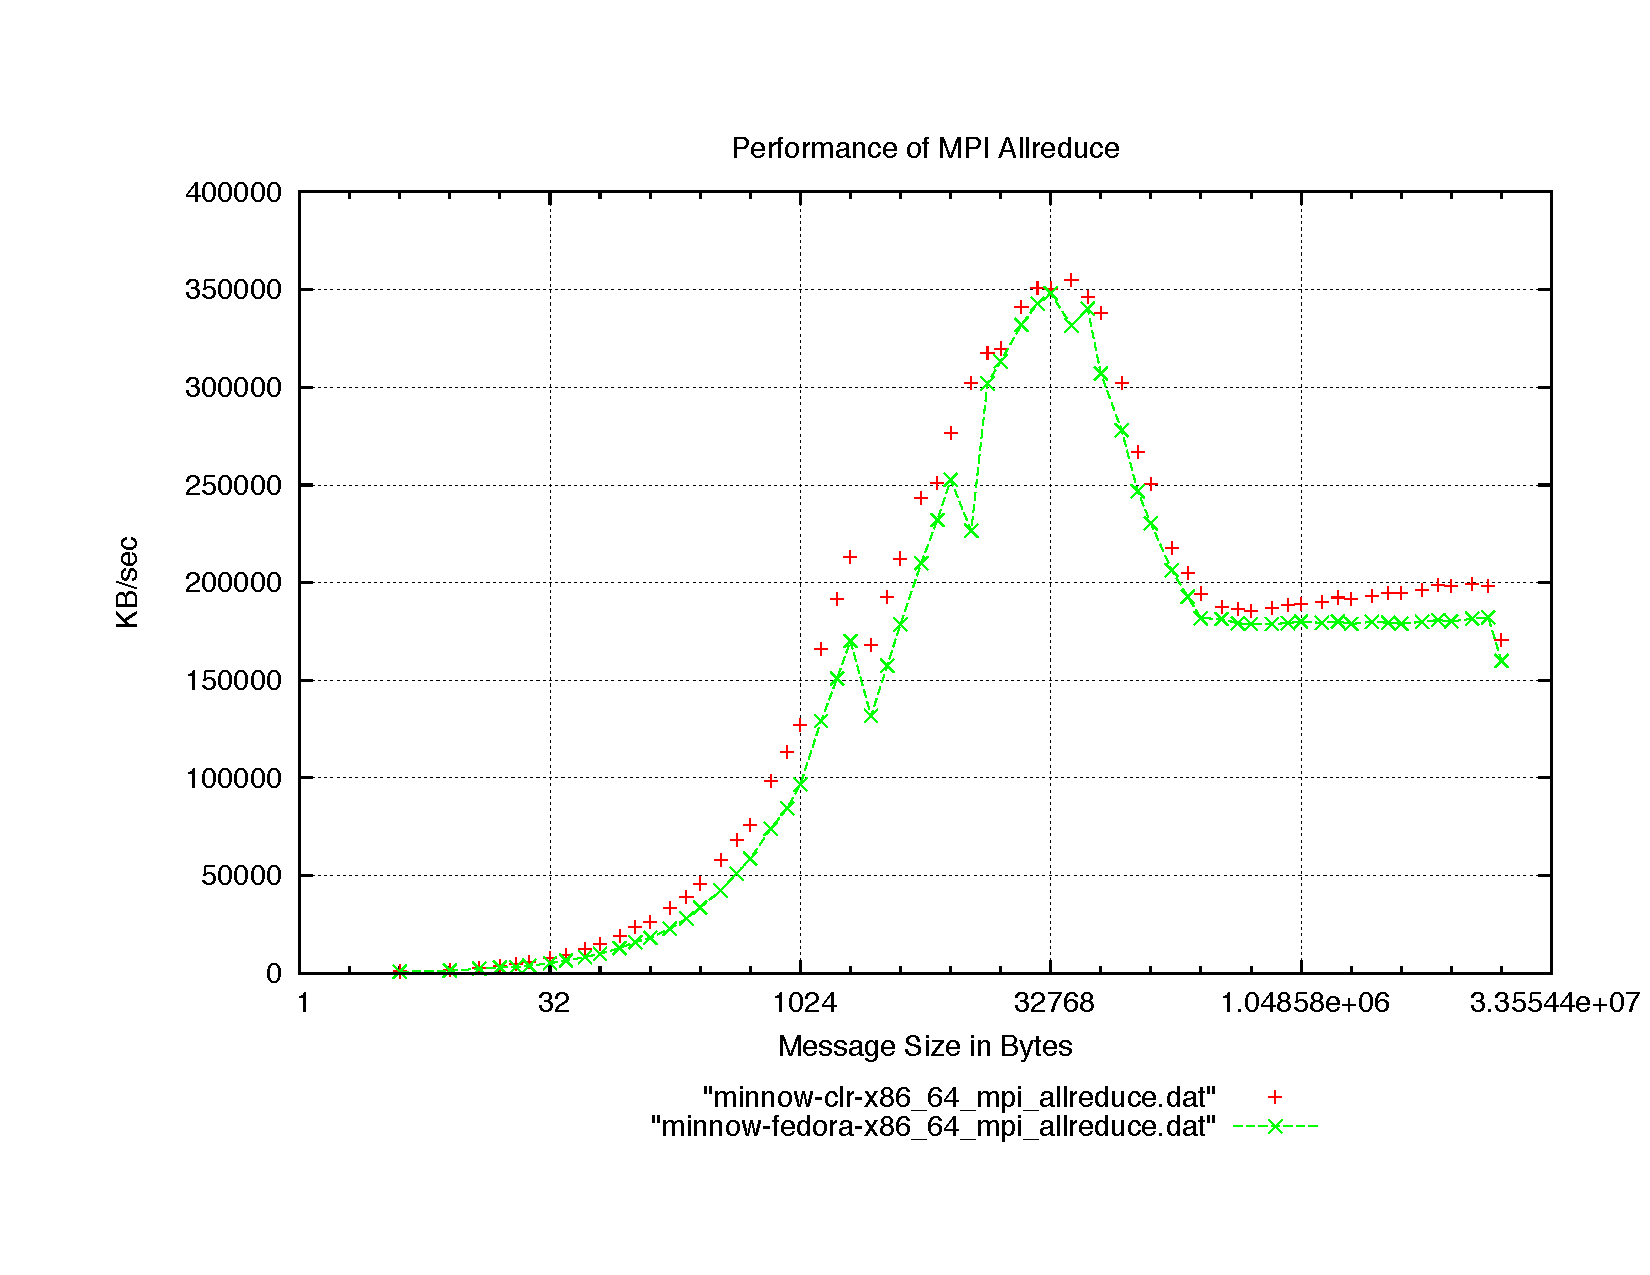
\includegraphics[width=\paperwidth]{images/mpbench_clr_experiments/mpi_allreduce.pdf}
\caption{\textit{MPI all reduce} benchmark running in MinnowBoard MAX with Clear Linux and
Fedora.}
\label{mpi_allreduce_clr_fedora}
\end{sidewaysfigure}

In Figure~\ref{mpi_allreduce_clr_fedora}, the \textit{all reduce} benchmark
shows more stable performance running in a customized OS. This can be seen in
the drop of speed (KB/sec) close to the test with a message size of 32 KB. 

\begin{sidewaysfigure}
  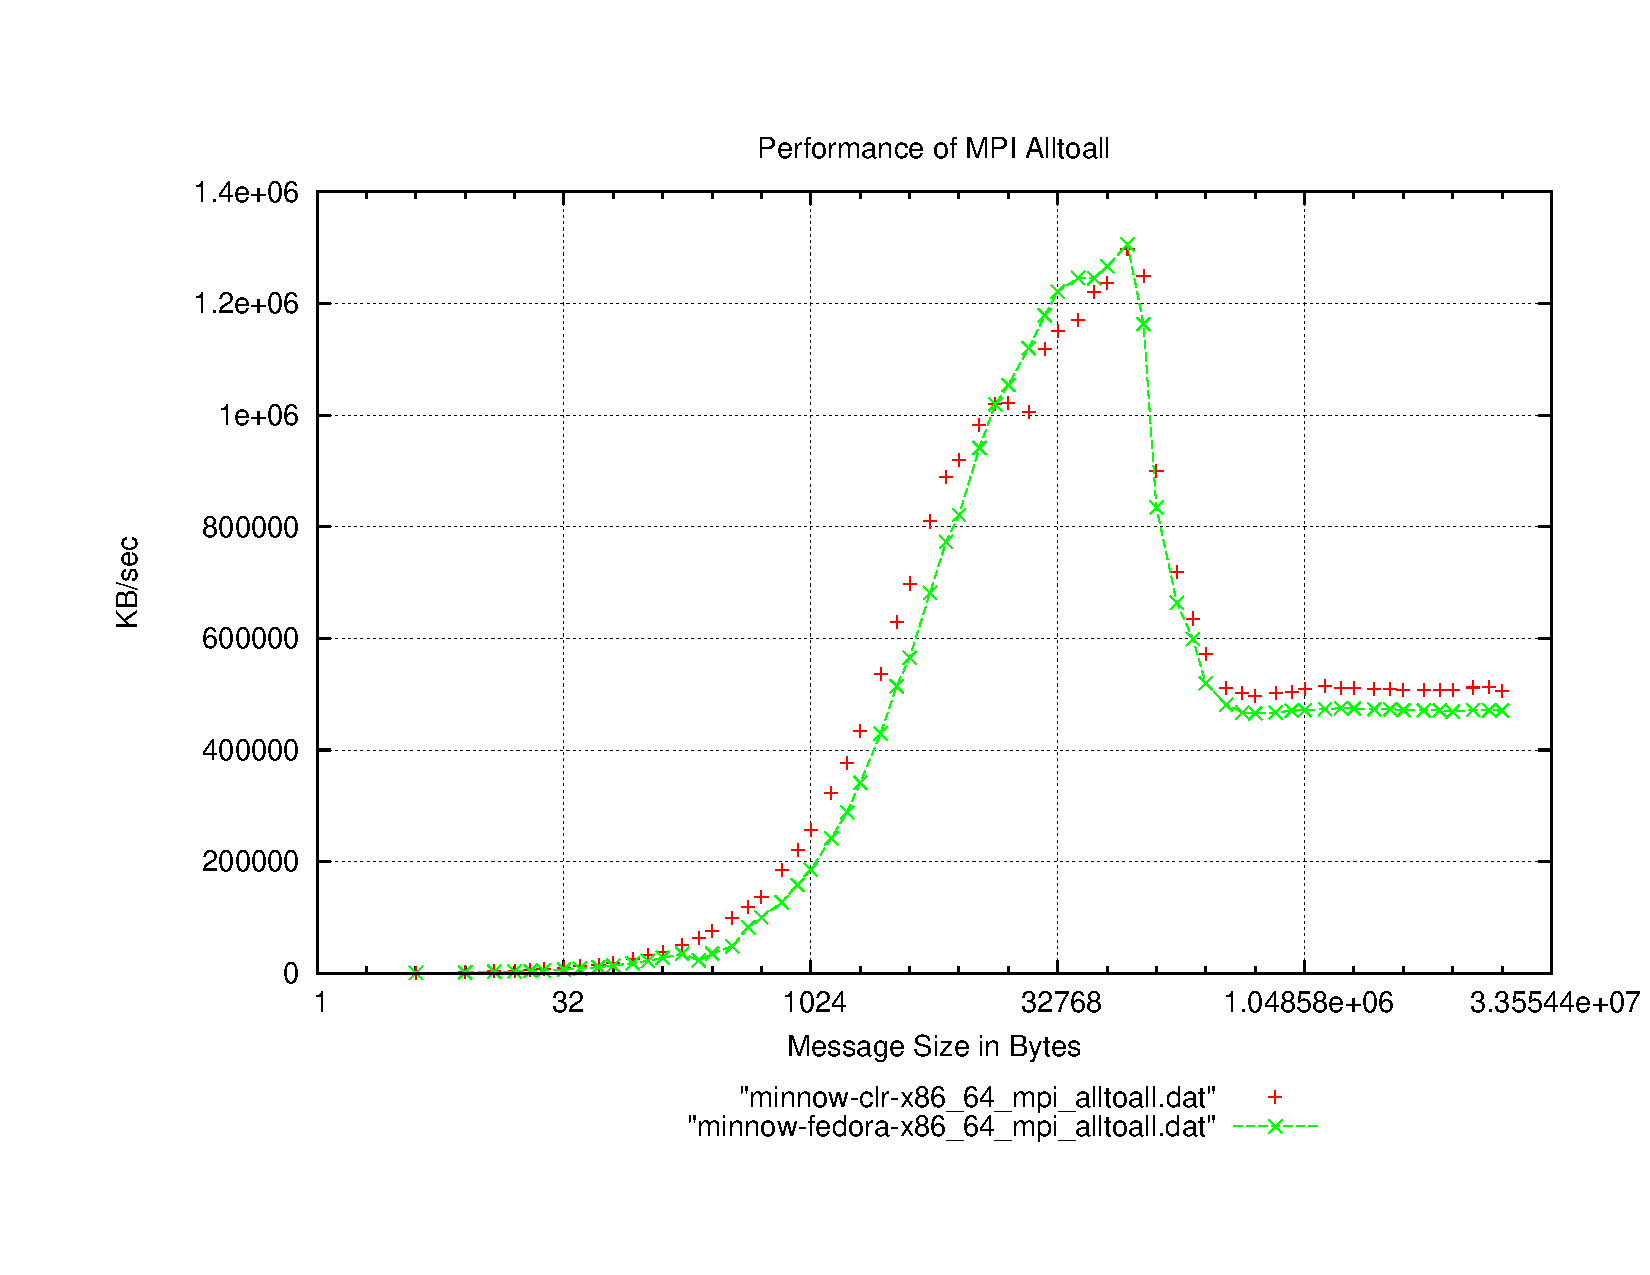
\includegraphics[width=\paperwidth]{images/mpbench_clr_experiments/mpi_alltoall.pdf}
\caption{\textit{MPI all to all} benchmark running in MinnowBoard MAX with Clear Linux and
Fedora.}
\label{mpi_alltoall_clr_fedora}
\end{sidewaysfigure}

In Figure~\ref{mpi_alltoall_clr_fedora}, the \textit{all to all} benchmark
shows the same performance running in a customized OS than in the Fedora OS. 

\begin{sidewaysfigure}
 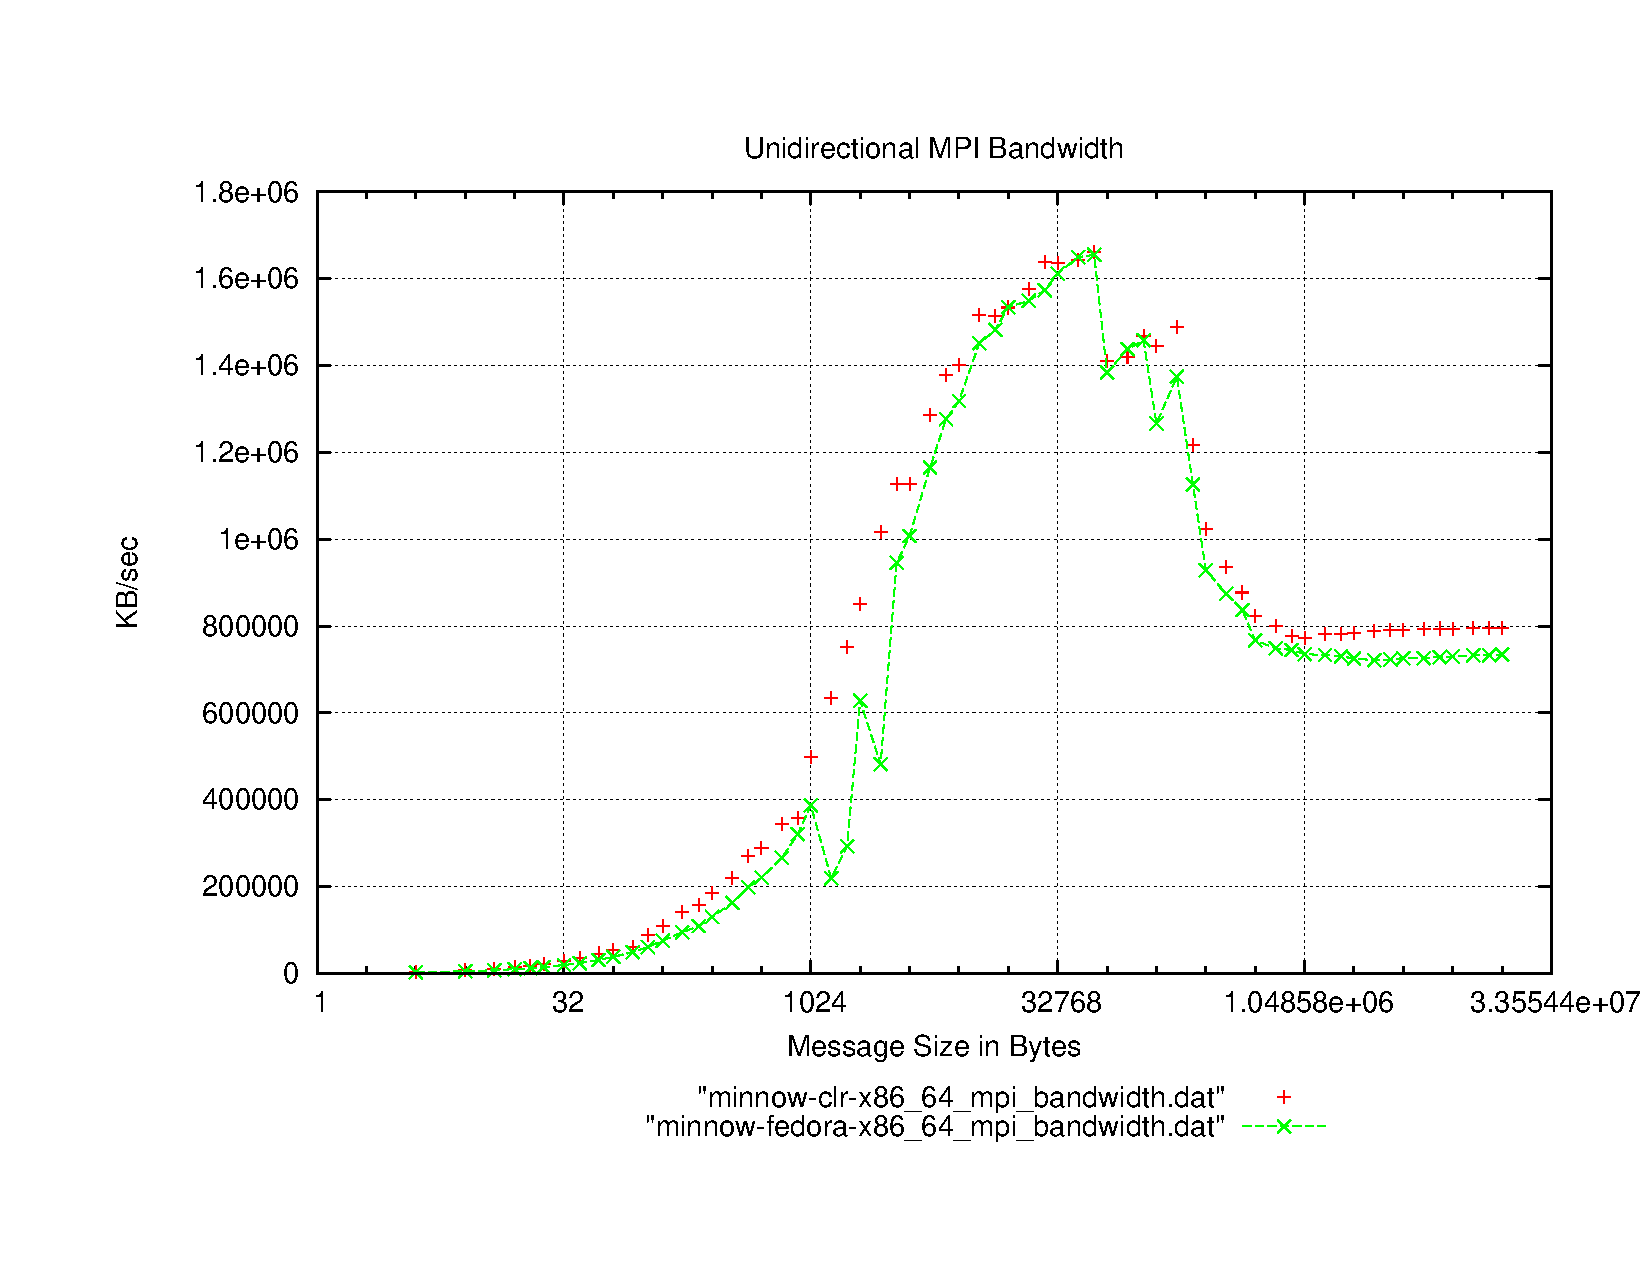
\includegraphics[width=\paperwidth]{images/mpbench_clr_experiments/mpi_bandwidth.pdf}
\caption{\textit{MPI bandwidth} benchmark running in MinnowBoard MAX with Clear Linux and
Fedora.}
\label{mpi_bandwidth_clr_fedora}
\end{sidewaysfigure}

The same results as presented in Figure \ref{mpi_allreduce_clr_fedora} can bee
seen in the \textit{bandwidth} benchmark (Figure
\ref{mpi_bandwidth_clr_fedora}); however, in the \textit{all to all} (Figure
\ref{mpi_alltoall_clr_fedora}) there are no drops in speed at any size of the
message under test.  This is mainly because of the nature of the test
(Described in Chapter 3). The \textit{all reduce} and the \textit{bandwidth}
tests execute similar tasks. Meanwhile, \textit{bandwidth} executes send and
receives.

On the other hand MPI \textit{all reduce} will reduce the values and distribute
the results to all processes. MPI \textit{all reduce} operates in each process
and then broadcasts the result of the operation to all the individuals of the
distributed system.

The Clear Linux OS has specific implementations in the kernel that improve the
network performance, specially in the kernel network area.

On the other hand, the \textit{all to all} sends data from all the nodes, this
means that each node of the system needs to send and receive data to every
other node. This increases the latency of the network.

\begin{sidewaysfigure}
  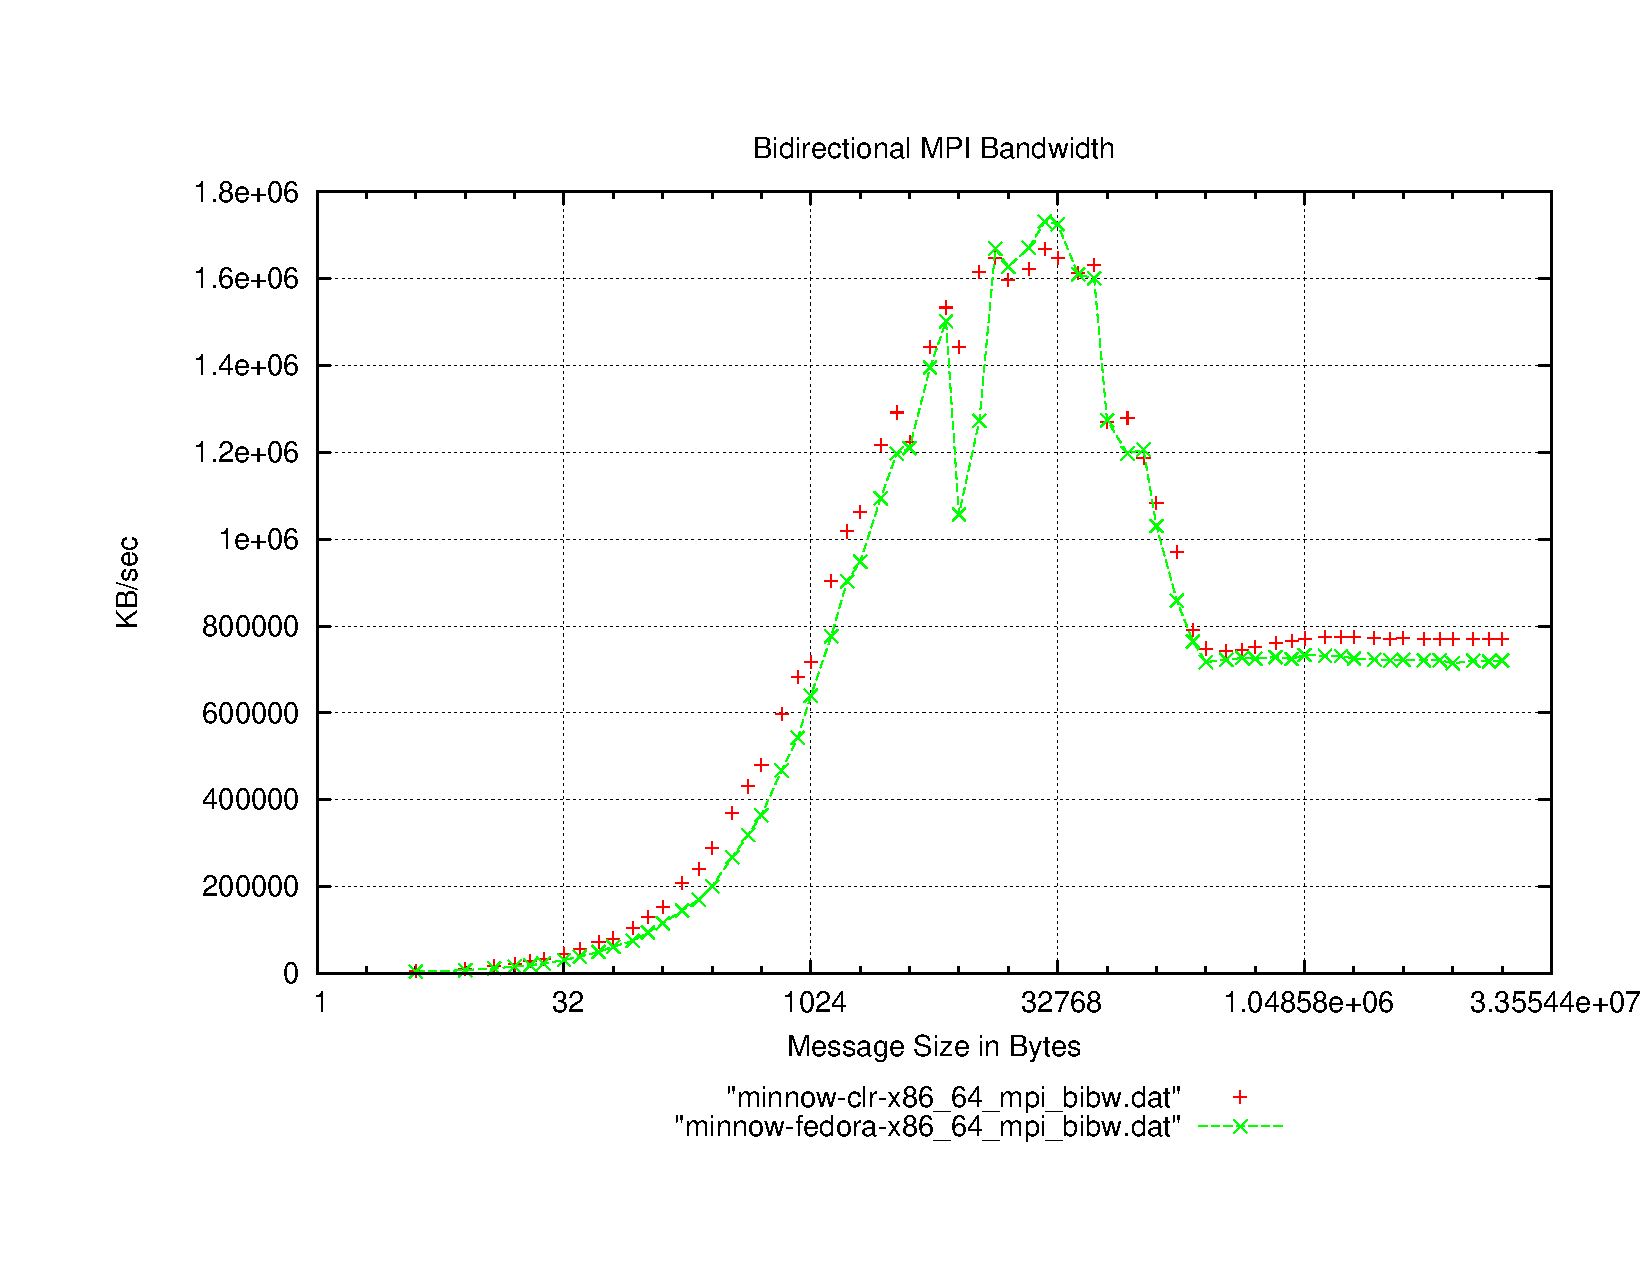
\includegraphics[width=\paperwidth]{images/mpbench_clr_experiments/mpi_bibw.pdf}
\caption{\textit{MPI Bi directional} bandwidth running in  MinnowBoard MAX with Clear Linux
and Fedora.}
\label{mpi_bibw_clr_fedora}
\end{sidewaysfigure}


The same results can be seen in the \textit{bi directional bandwidth} (Figure
\ref{mpi_bibw_clr_fedora}) and the \textit{broadcast} (Figure
\ref{mpi_broadcast_clr_fedora}) test. 

\begin{sidewaysfigure}
  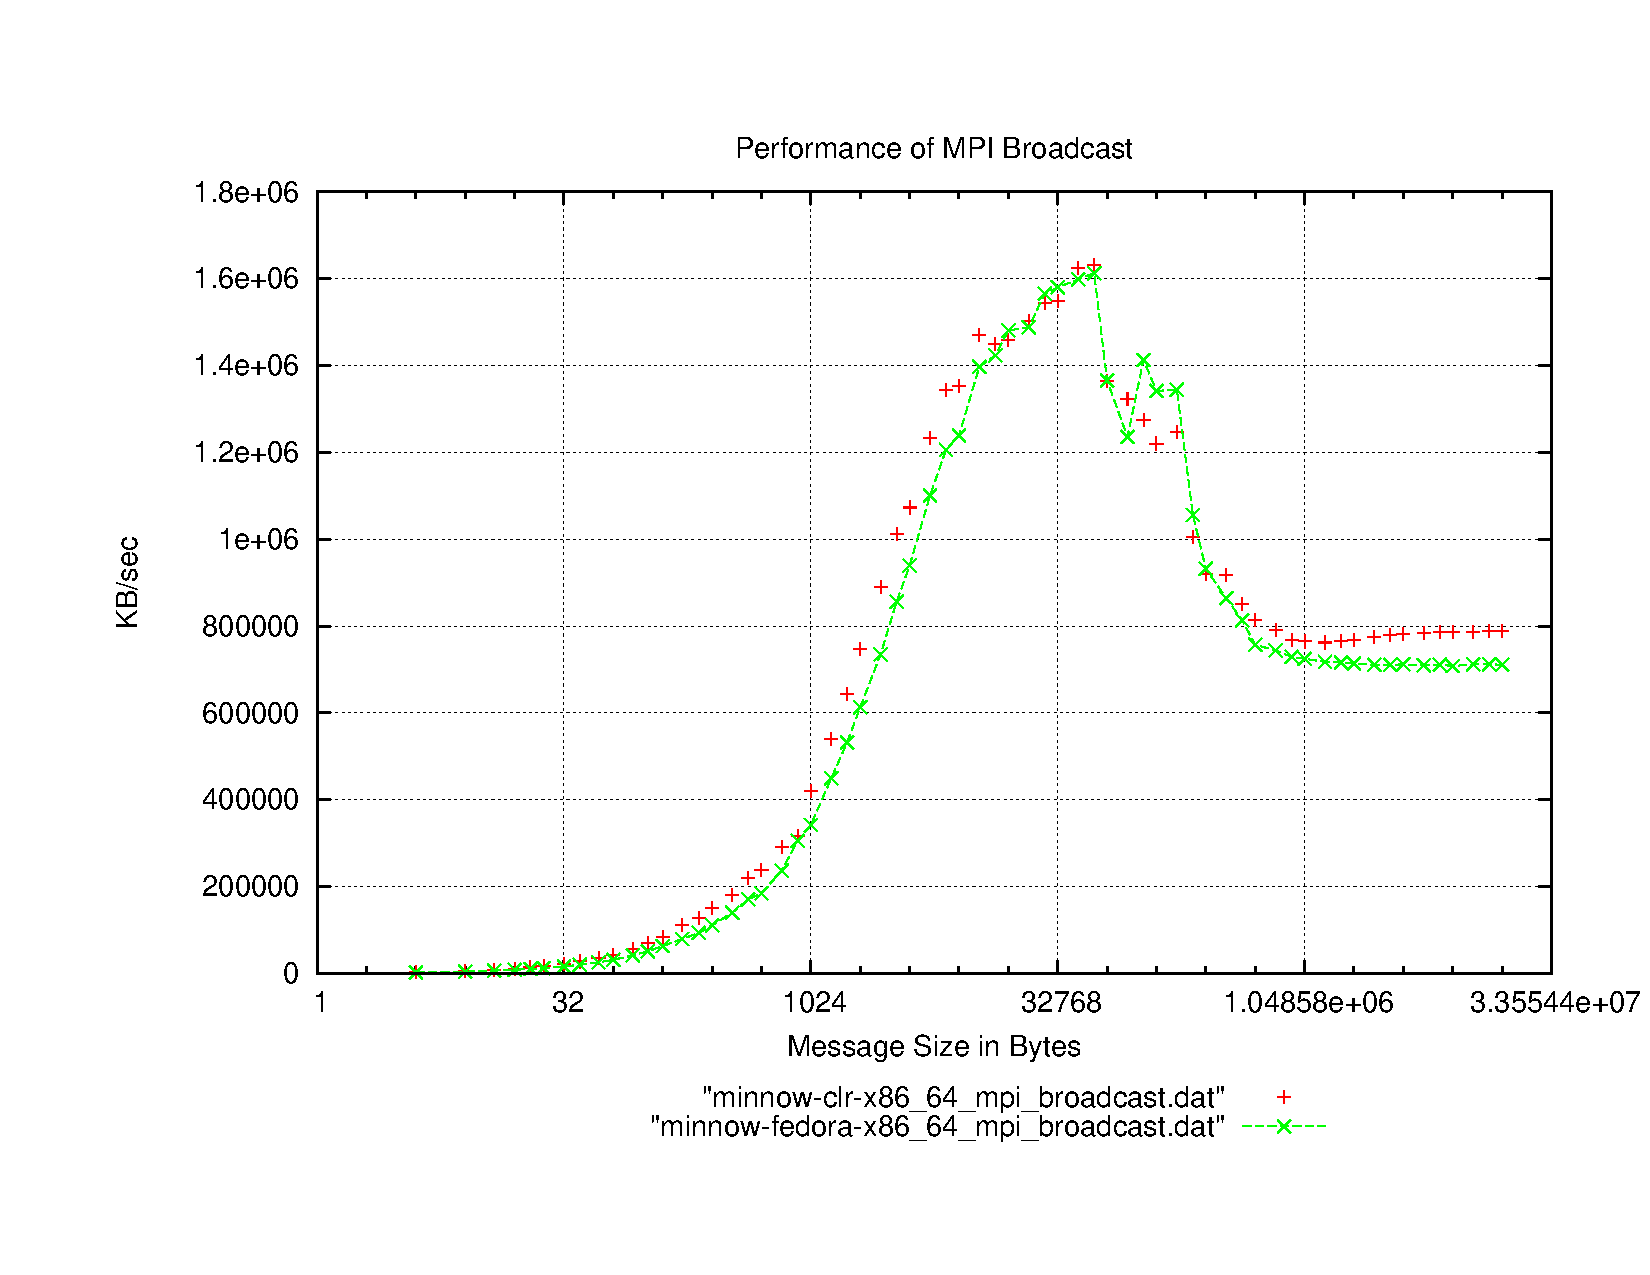
\includegraphics[width=\paperwidth]{images/mpbench_clr_experiments/mpi_broadcast.pdf}
\caption{\textit{MPI broadcast} benchmark running in  MinnowBoard MAX with Clear Linux and
Fedora (higher is better)}
\label{mpi_broadcast_clr_fedora}
\end{sidewaysfigure}

The MPBench measures bidirectional bandwidth with a nested loop. The outer loop
varies the message size, and the inner loop measures the send operation over
the iteration count. Both processes execute a non-blocking receive, then a
non-blocking send.  A non blocking send and receive means that each process
will release the communication channel to other processes. If we check the
number of processes running in Fedora , the number is 30\% higher. This can bee
seen in the Figure \ref{number_forks_fedora_clr}

\begin{figure}[H]
\centering
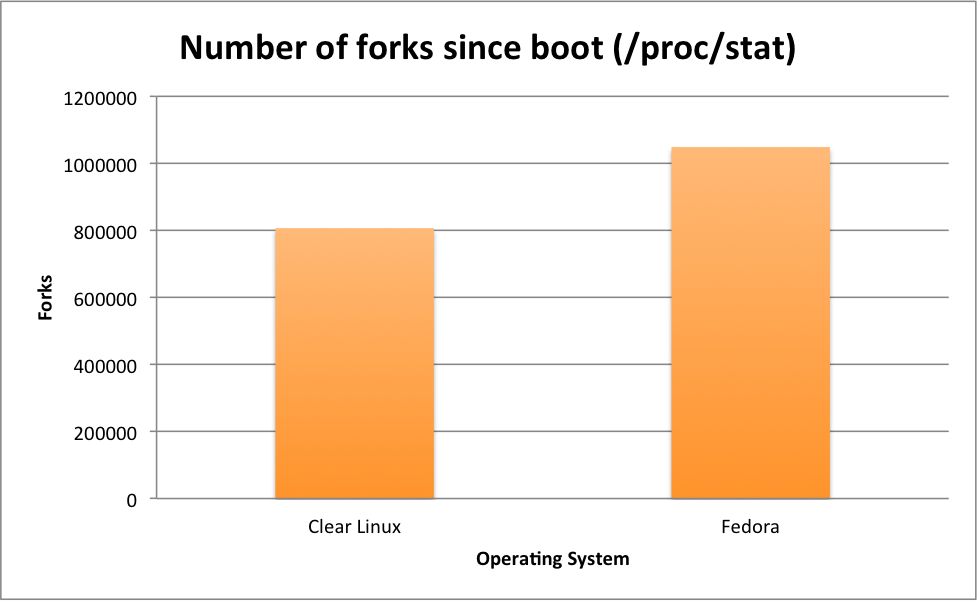
\includegraphics[width=1 \textwidth]{images/number_forks.png}
\caption{Number of forks since booting process reported in /proc/stat file }
\label{number_forks_fedora_clr}
\end{figure}

The \textit{latency} benchmark can be described as one that measures the time
for an application to issue a send and continue computing (More details in
Chapter 3). 

Figure \ref{mpi_latency_clr_fedora} shows the latency in both operating systems
is similar. The significant change is at the beginning of the test (before the
package size reach be 32 Bytes). This is due to the fact that the test includes
one system, therefore there is no network message. It does not have
to travel through multiple points due to the simplicity of the cluster network
(the send message is received immediately) 

\begin{sidewaysfigure}
  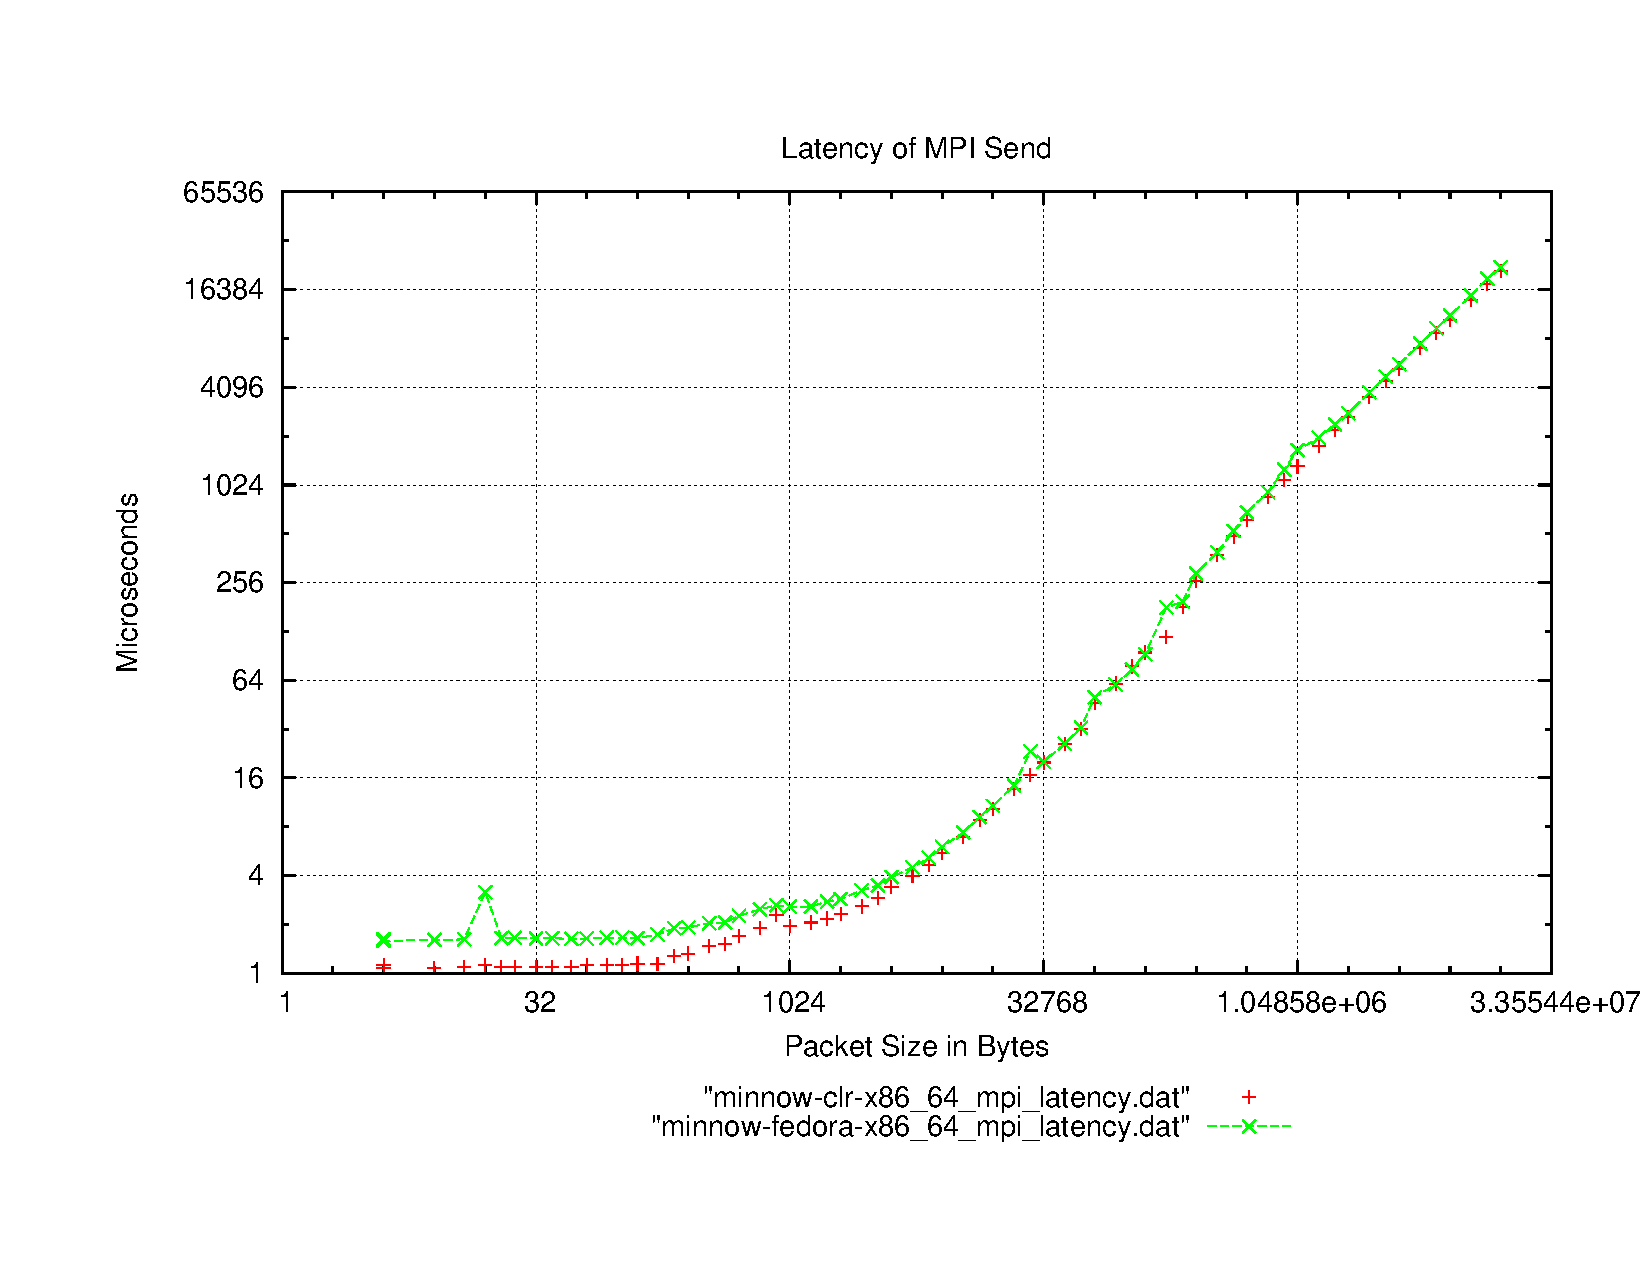
\includegraphics[width=\paperwidth]{images/mpbench_clr_experiments/mpi_latency.pdf}
\caption{\textit{MPI latency} benchmark running in  MinnowBoard MAX with Clear Linux and
Fedora}
\label{mpi_latency_clr_fedora}
\end{sidewaysfigure}

Roundtrip times are measured in much the same way as \textit{bandwidth}, except
that, the slave process, after receiving the message, echoes it back to the
master. No acknowledgment is needed with this test as it is implicit given its
semantics. The master's pseudo code for this test is described in Chapter 3.

Similar results to \textit{roundtrip} test are shown in Figure \ref{mpi_roundtrip_clr_fedora}

\begin{sidewaysfigure}
  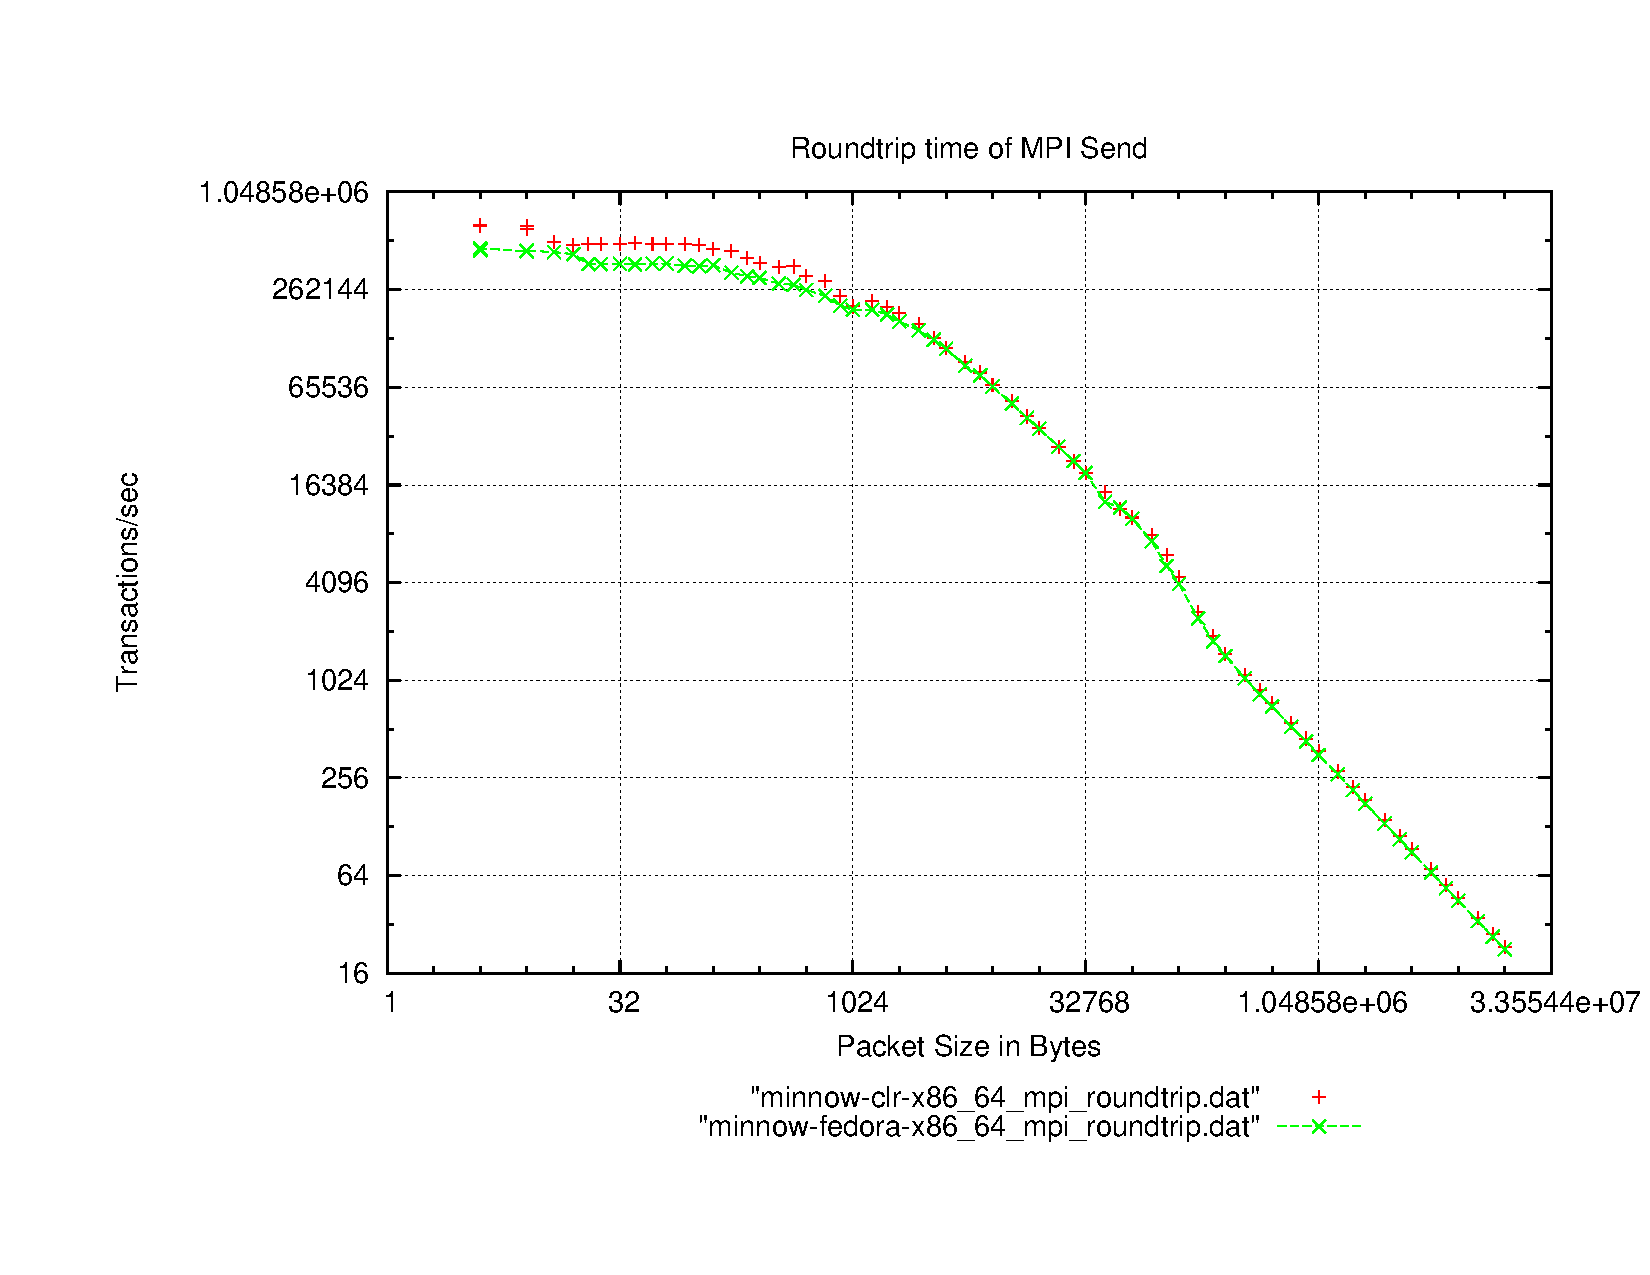
\includegraphics[width=\paperwidth]{images/mpbench_clr_experiments/mpi_roundtrip.pdf}
\caption{\textit{MPI Roundtrip} benchmark running in MinnowBoard MAX with Clear Linux and
Fedora.}
\label{mpi_roundtrip_clr_fedora}
\end{sidewaysfigure}

Based on the results from these experiments it can be observed that customized 
operating system provides benefits to a cluster of embedded platforms. Experiments 
with two operating systems, one commercial (Fedora) and one customized (Clear
linux for Intel Architecture). It was worth trying with an operating system
designed for embedded and IoT platforms. 

The standard of the embedded industry to generate a custom Linux OS
is the Yocto project. In table~\ref{tab:3.2}, the operating systems
generated with the Yocto project do not have an implementation of the MPI
library.

To implement MPI experiments using Yocto is necessary to port the MPI
implementation.


\section{Porting MPI to Yocto}

The system under test (Hardware and Software) for this experiment is described
in the Table~\ref{tab:mpi_multiple_os_yocto}

    \begin{center}
    \begin{tabular}{ | l | r |}
        \hline
        \textbf{Platform under test} & Minnow Board  Max \\ \hline
        \textbf{Number of platforms} & 1  \\ \hline
        \textbf{Operating System} & Fedora, Clear Linux and Yocto  \\ \hline
    \end{tabular}
    \captionof{table}{Description of system under test (HW/SW) for MPI
    benchmark evaluation on Yocto}\label{tab:mpi_multiple_os_yocto}
    \end{center}

The Yocto project \cite{yocto-project} generates a custom Linux OS for
embedded systems. The way to add a new capability to the system is by adding a
new receipt. This is described in the Yocto documentation. In order to make the
Yocto evaluation it was necessary to implement MPI in Yocto. The receipt
implemented for MPI is shown in Figure \ref{mpi_yocto}

\begin{minipage}{\textwidth}
\end{minipage}

\begin{minipage}{\textwidth}

\begin{lstlisting}[frame=single,numbers=left,breaklines=true]
SUMMARY = "Message Passing Interface (MPI) implementation"
HOMEPAGE = "http://www.mpich.org/"
SECTION = "devel"

LICENSE = "BSD-2-Clause"
LIC_FILES_CHKSUM = "file://COPYRIGHT;md5=2106f0435056f3dd9349747a766e5816"

SRC_URI = " \
	http://www.mpich.org/static/downloads/${PV}/mpich-${PV}.tar.gz \
"
SRC_URI[md5sum] = "40dc408b1e03cc36d80209baaa2d32b7"
SRC_URI[sha256sum] = "455ccfaf4ec724d2cf5d8bff1f3d26a958ad196121e7ea26504fd3018757652d"
CACHED_CONFIGUREVARS += "BASH_SHELL=${base_bindir}/bash"

RDEPENDS_${PN} += "bash perl libxml2"
S = "${WORKDIR}/${BP}"

EXTRA_OECONF = "--enable-debuginfo --enable-fast \
                --enable-shared --with-pm=gforker  \
		        --disable-rpath --disable-f77 \
                --disable-fc --disable-fortran --disable-cxx"

inherit autotools-brokensep gettext

do_configure_prepend() {
    autoreconf --verbose --install --force -I . -I confdb/ -I maint/
    oe_runconf
    exit
}

\end{lstlisting}
\captionof{figure}{Receipt to enable MPI libraries in Yocto operating systems}
\label{mpi_yocto} 
\end{minipage}

\newpage

This receipt is part of the meta-openembedded layer, (
\url{http://cgit.openembedded.org/cgit.cgi/meta-openembedded/tree/meta-oe/recipes-devtools/mpich/mpich_3.1.1.bb?h=master})
a layer for all the embedded tools that the Linux distributions might need, in this
layer the user can add editors and other libraries that the embedded
application might need.

The core of the developed MPI implementation for this work consist in the
configuration part. The configuration is described in the ''EXTRA\_OECONF''. 
The reasons for that are: 

\begin{itemize}
\item \textit{enable-debuginfo}: For debugging the system when needed
\item \textit{enable-fast}: Turns off error checking and collection of internal timing
information
\item \textit{eenable-shared}; Enable shared library support in order to split the MPI
capabilities in multiple binaries and shared object libraries . This makes the
compiler and process manager applications smaller in size.
\item \textit{ewith-pm=gforker}: The gforker process manager is primarily intended as a
debugging aid as it simplifies development and testing of MPI programs on a
single node or processor.
\item \textit{edisable-rpath} : Do not link static libraries, if so the build
applications generated by this MPI implementation will not run in other MPI
systems with different paths to libraries.
\item \textit{edisable-f77}: Build the Fortran 77 bindings (enabled by default).
\item \textit{edisable-fc}: Build the Fortran 90 bindings (enabled by default),
This work is not supporting Fortran, it was needed to disable it.
\item \textit{edisable-fortran}: Yocto project does not support Fortran.
\item \textit{edisable-cxx}: Build the C++ bindings (enabled by default). This
work does not support C++ to generate a small MPI implementation.
\end{itemize}


\subsection{Results}

With this configuration it was created an MPI implementation for Yocto, 
not just the compiler, but also the MPI process manager. The results of
doing this can be seen in the following graphs of the MPI benchmarks, now
running with a Yocto base image.

\begin{sidewaysfigure}
  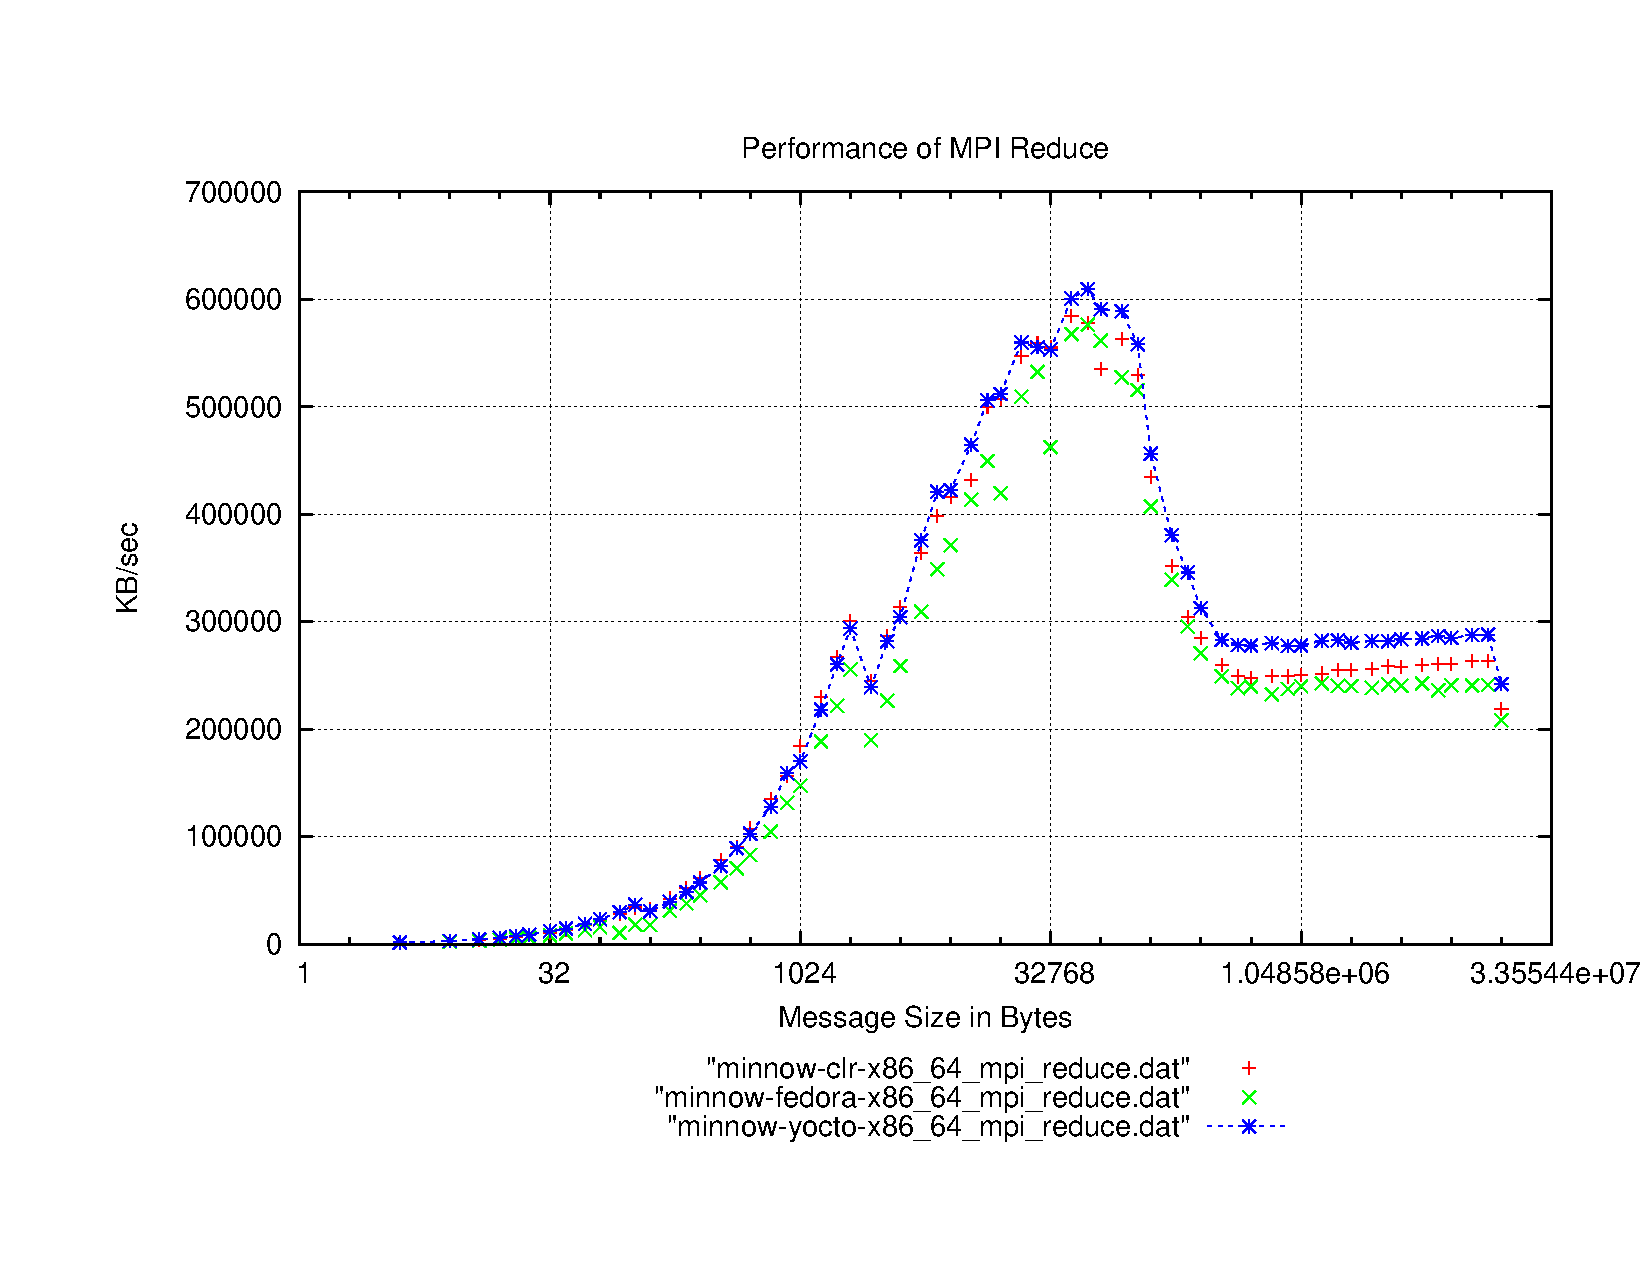
\includegraphics[width=\paperwidth]{images/mpbench_yocto_experiments/mpi_reduce.pdf}
\caption{MPI Reduce benchmark running in MinnowBoard MAX with Clear Linux, Yocto
and Fedora.}
\label{mpi_reduce_yocto}
\end{sidewaysfigure}

The performance of \textit{MPI reduce} test is similar despite the operating
system is installed on the platform. This can be seen in the Figure
\ref{mpi_reduce_yocto}.

\begin{sidewaysfigure}
  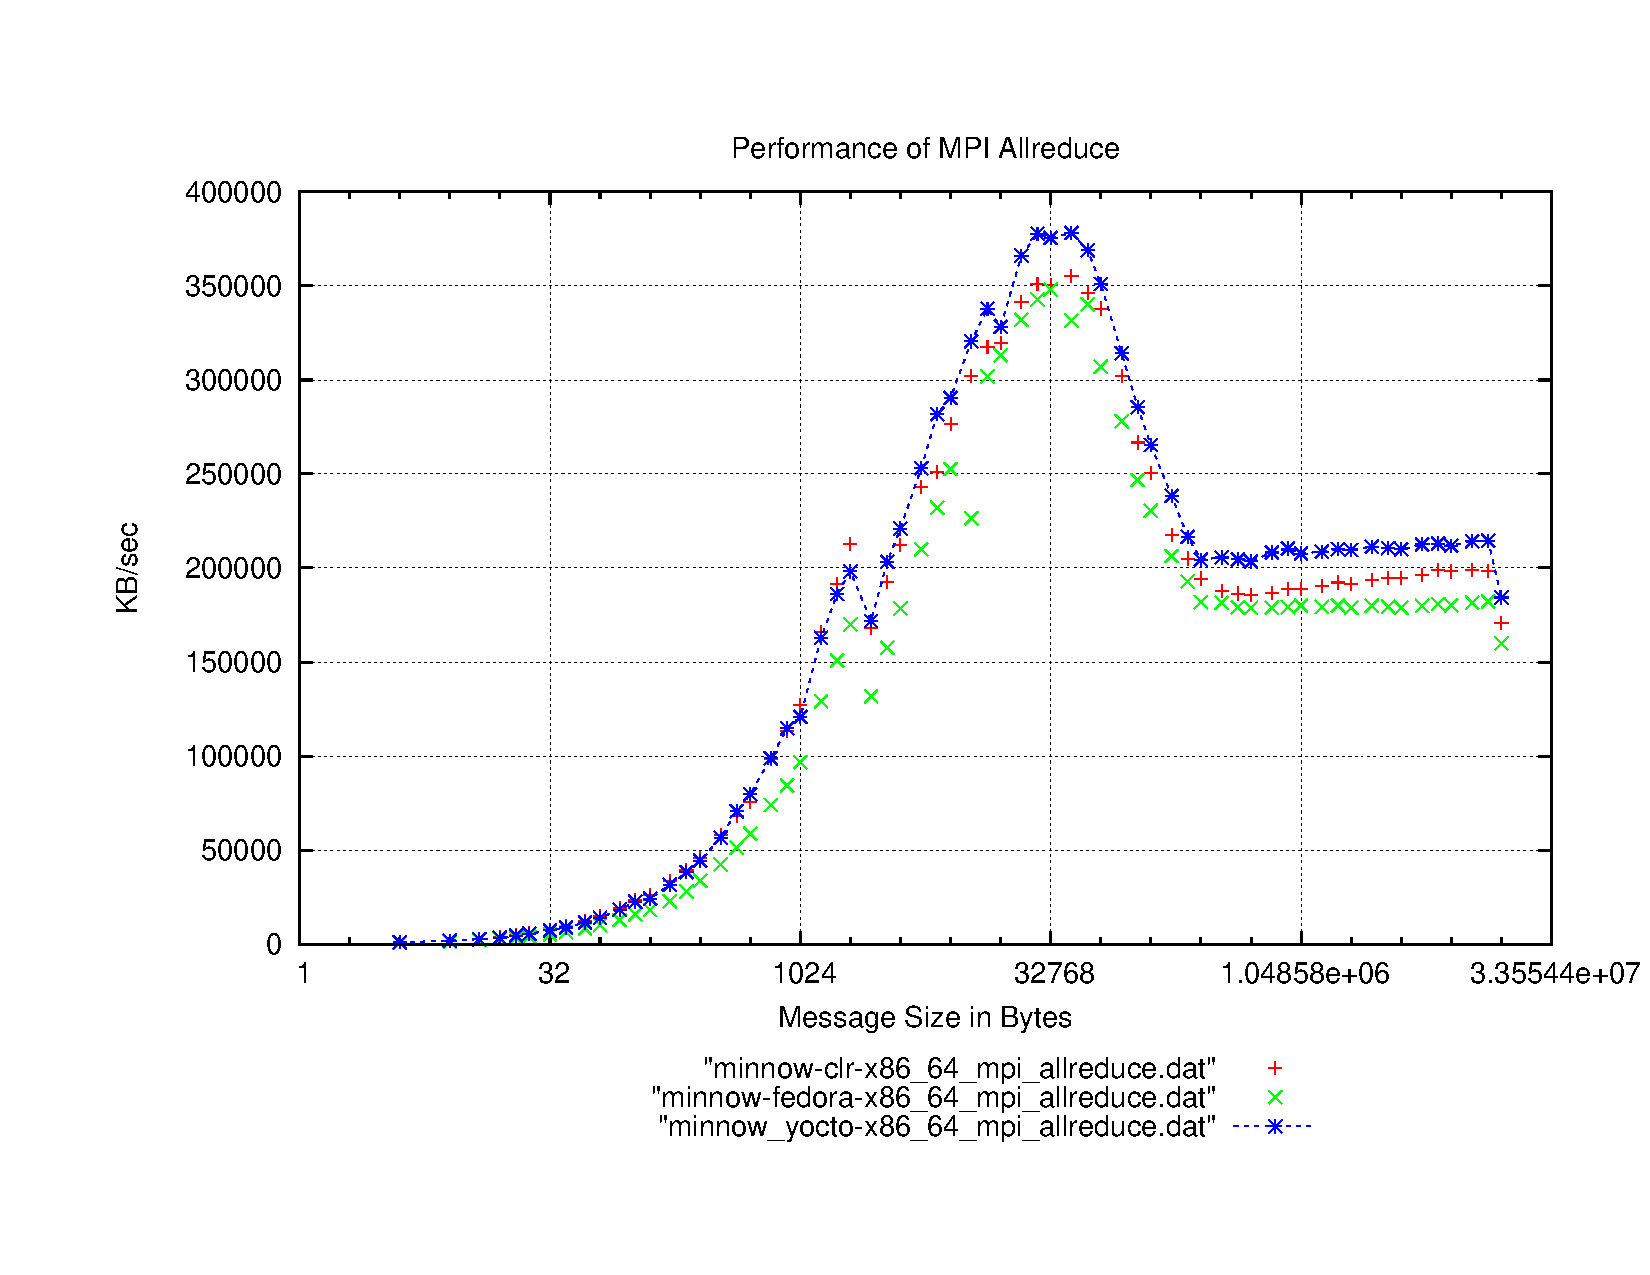
\includegraphics[width=\paperwidth]{images/mpbench_yocto_experiments/mpi_allreduce.pdf}
\caption{\textit{MPI all reduce} benchmark running in  MinnowBoard MAX with Clear Linux,
Yocto and Fedora (higher is better)}
\label{mpi_allreduce_yocto}
\end{sidewaysfigure}

The performance of \textit{MPI all reduce} test is grater with the Yocto based
operating system. This can be seen in the Figure \ref{mpi_allreduce_yocto}.

\begin{sidewaysfigure}
  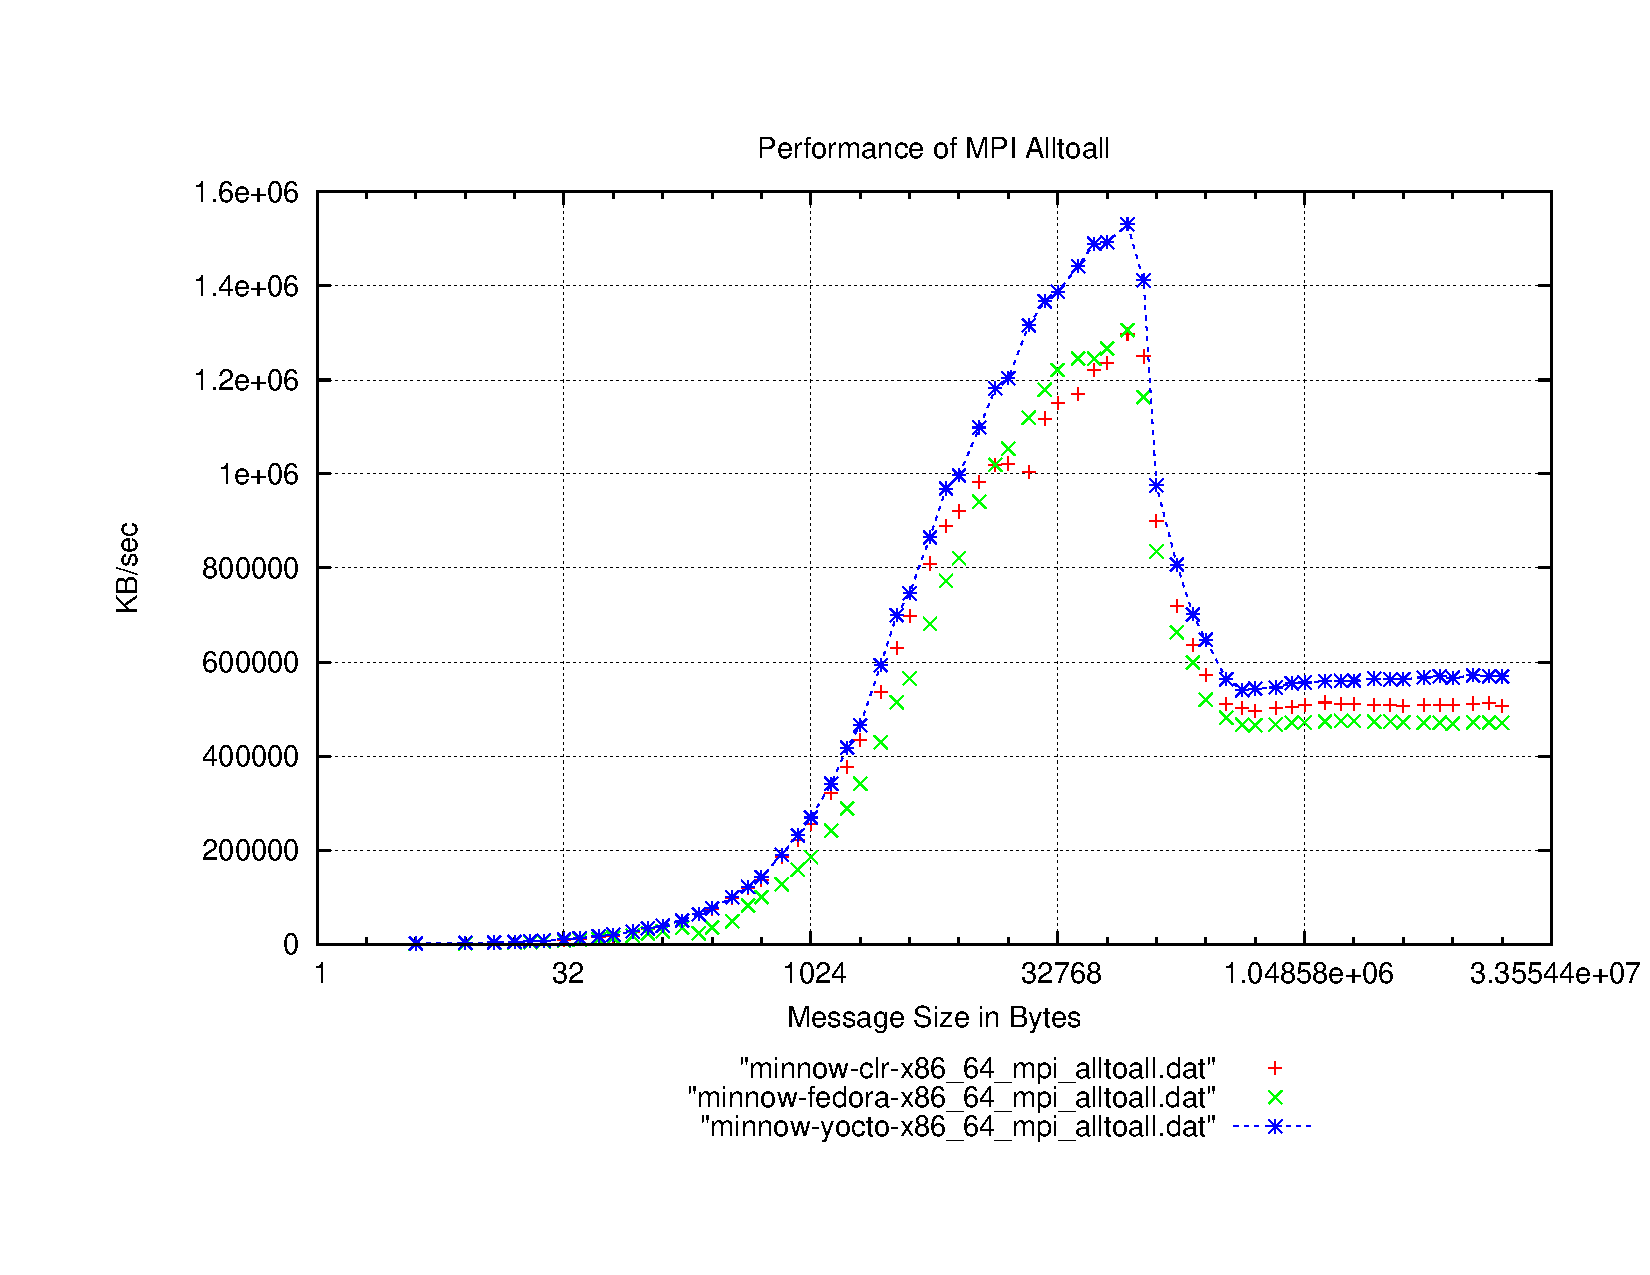
\includegraphics[width=\paperwidth]{images/mpbench_yocto_experiments/mpi_alltoall.pdf}
\caption{\textit{MPI all to all} benchmark running in  MinnowBoard MAX with Clear Linux, Yocto
and Fedora (higher is better)}
\label{mpi_all_to_all_yocto}
\end{sidewaysfigure}

The results with the Yocto based operating system have the same
tendency that with the Clear Linux OS. Excepting  the \textit{all to all}
experiment, where the gain in performance was higher with a message size
larger than 32 KB. This is because of the test measures a round-robin communication 
between multiple processes \footnote{More information regarding to \textit{all
to all} test in Chapter 3}.

MPI \textit{all to all} is a collective operation in which all processes send
the same amount of data to each other, and receive the same amount of data from
each other. Each process has its own data, at the end, all the processes have
the same amount of data. 

Each of the process are blocking processes, which means that the number of
processes does not affect the performance of the test. However,
the configuration of the Yocto Base operating system has 
some modifications for the specific tested platforms. Mainly in the
kernel section as it is shown in the Figure \ref{kernel_yocto}.

\begin{minipage}{\textwidth}
\end{minipage}

\begin{minipage}{\textwidth}
\begin{lstlisting}[frame=single,numbers=left]
    # enable cpu frequency scaling and stats for powertop
    CONFIG_CPU_FREQ=y
    CONFIG_CPU_FREQ_STAT=y
    CONFIG_X86_ACPI_CPUFREQ=y
    CONFIG_X86_INTEL_PSTATE=y
    CONFIG_CPU_FREQ_GOV_ONDEMAND=y
    CONFIG_CPU_FREQ_GOV_PERFORMANCE=y
    CONFIG_CPU_FREQ_DEFAULT_GOV_ONDEMAND=y
\end{lstlisting}
\captionof{figure}{Performance improvement in Kernel for Yocto operating
systems.}
\label{kernel_yocto} 
\end{minipage}

\begin{minipage}{\textwidth}
\end{minipage}

The Yocto kernel for the platform under test has the CPU clock frequency
scaling enable. Clock scaling allows to change the clock speed of CPUs at
runtime. This is a nice method to save battery during runtime, as well as, a
nice method to boost the speed of the system when required. In this case the
speed of the system is increased upon request when the send/receive method
requires it.


The performance of \textit{MPI bandwidth} test is higher with the Yocto based
operating system. This can be seen in the Figure \ref{mpi_bandwidth_yocto}.

\begin{sidewaysfigure}
  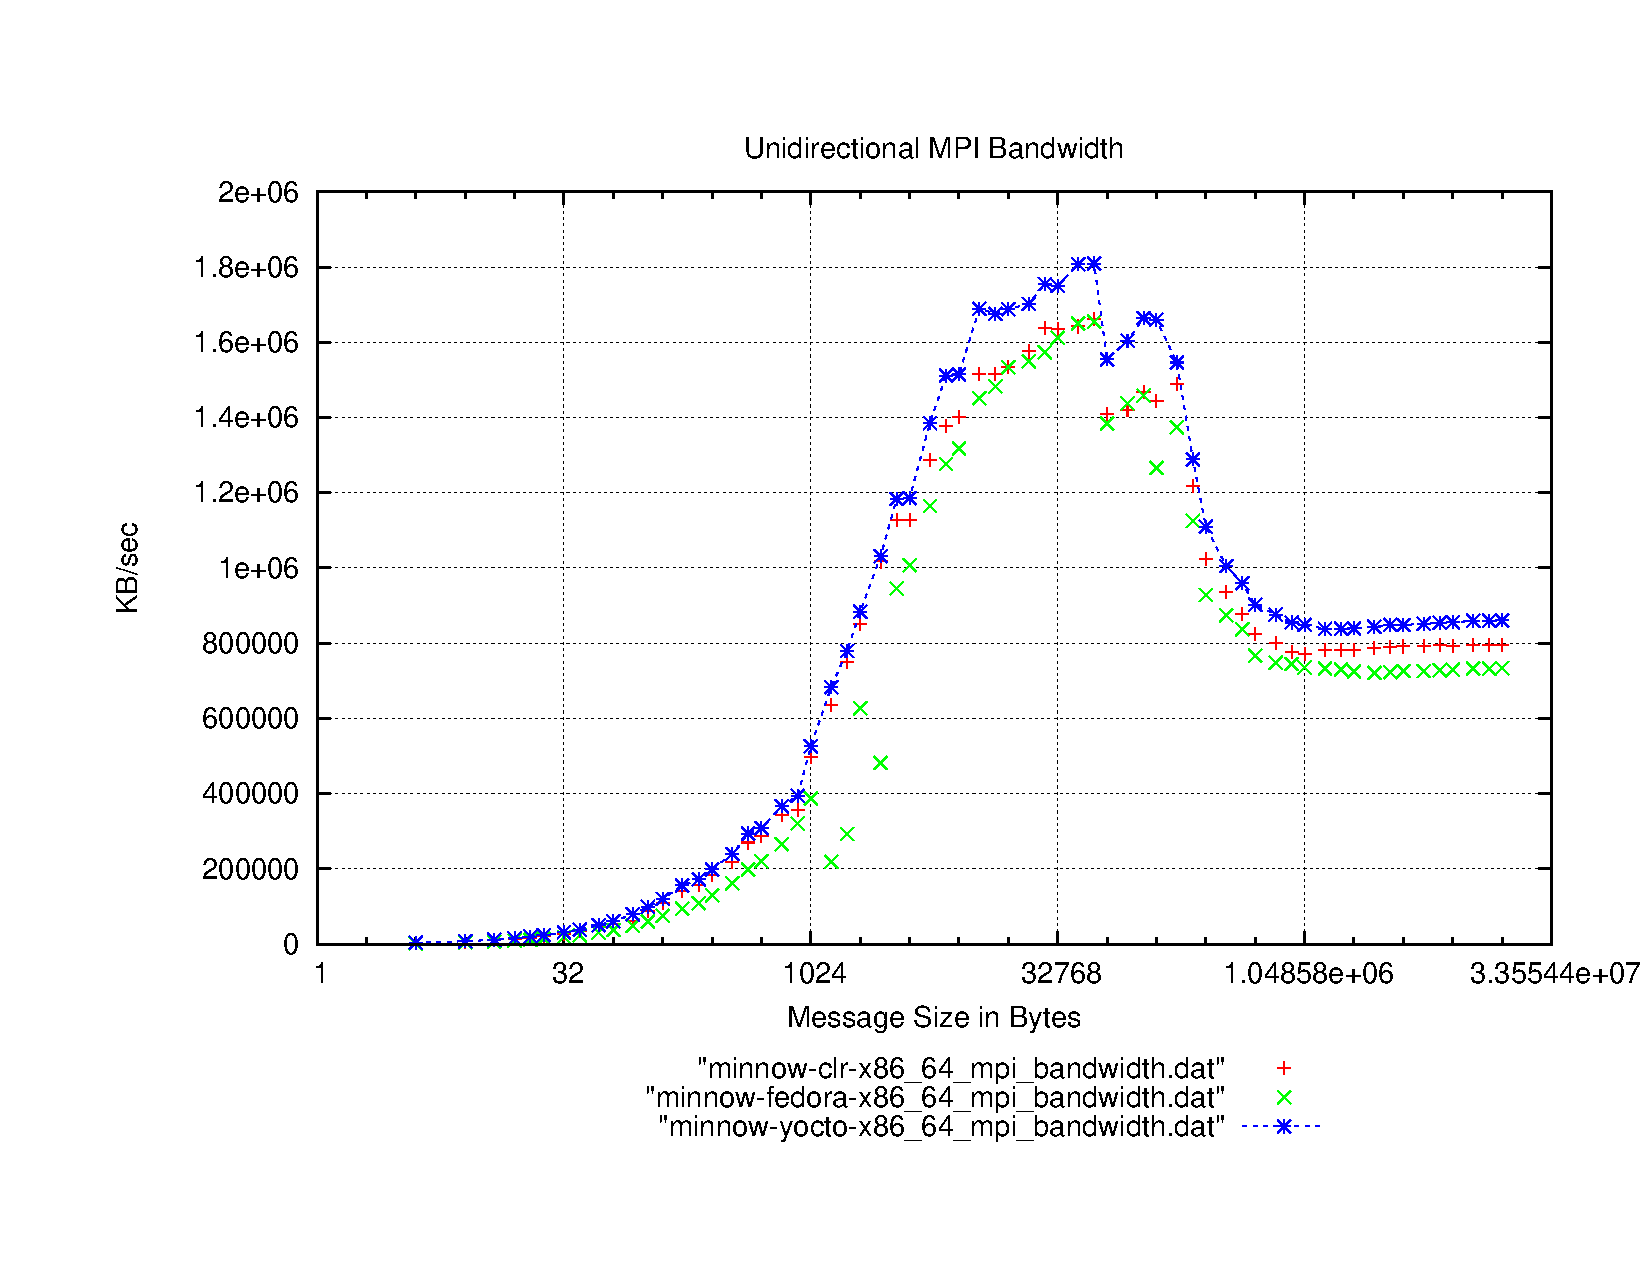
\includegraphics[width=\paperwidth]{images/mpbench_yocto_experiments/mpi_bandwidth.pdf}
\caption{\textit{MPI bandwidth} benchmark running in Minnowboard MAX with Clear Linux,
Yocto and Fedora.}
\label{mpi_bandwidth_yocto}
\end{sidewaysfigure}


Same result can be seen in Figure \ref{mpi_bibw_yocto} and
\ref{mpi_broadcast_yocto}. Specially after the
message size is 32KB. The test performance of the test \textit{MPI bandwidth}
is is higher due to the use of a Yocto operating system. 

\begin{sidewaysfigure}
  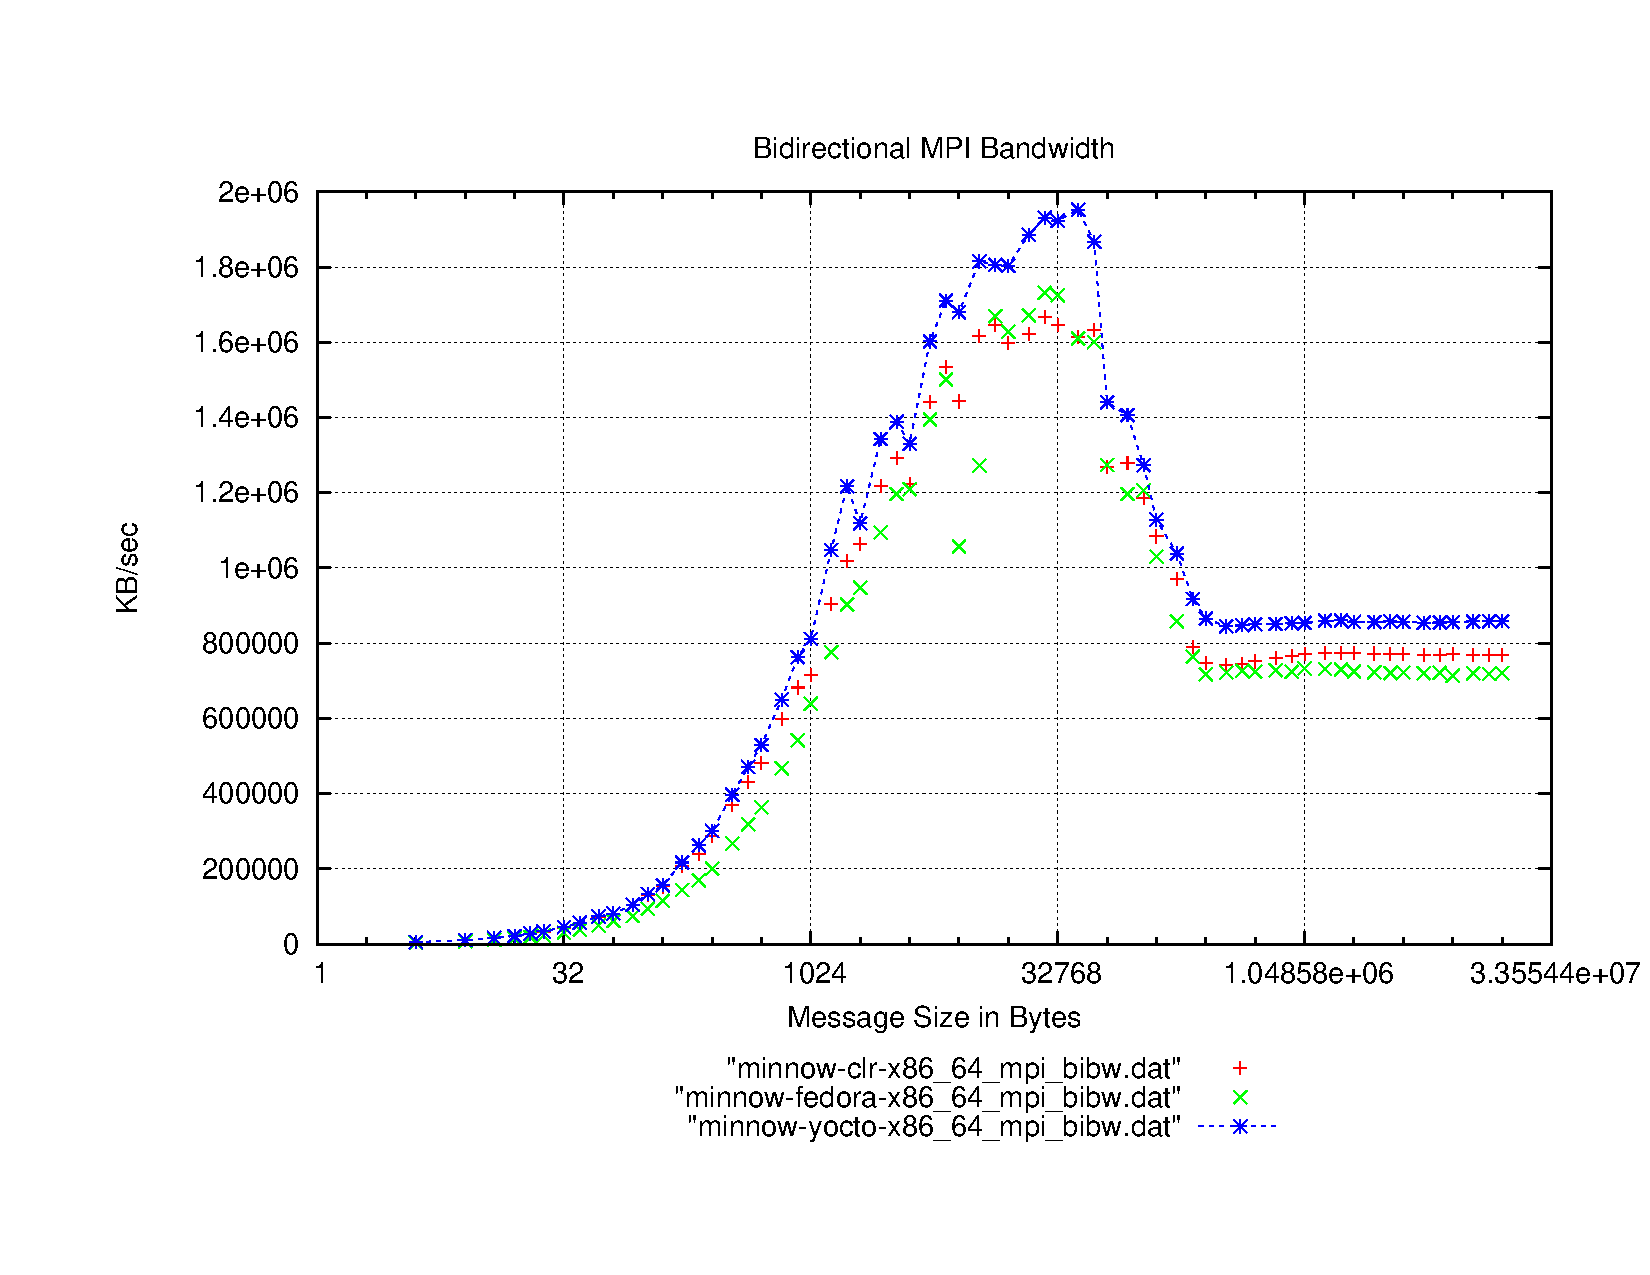
\includegraphics[width=\paperwidth]{images/mpbench_yocto_experiments/mpi_bibw.pdf}
\caption{\textit{MPI Bi directional} bandwidth running in MinnowBoard MAX with Clear Linux,
Yocto and Fedora.}
\label{mpi_bibw_yocto}
\end{sidewaysfigure}

\begin{sidewaysfigure}
  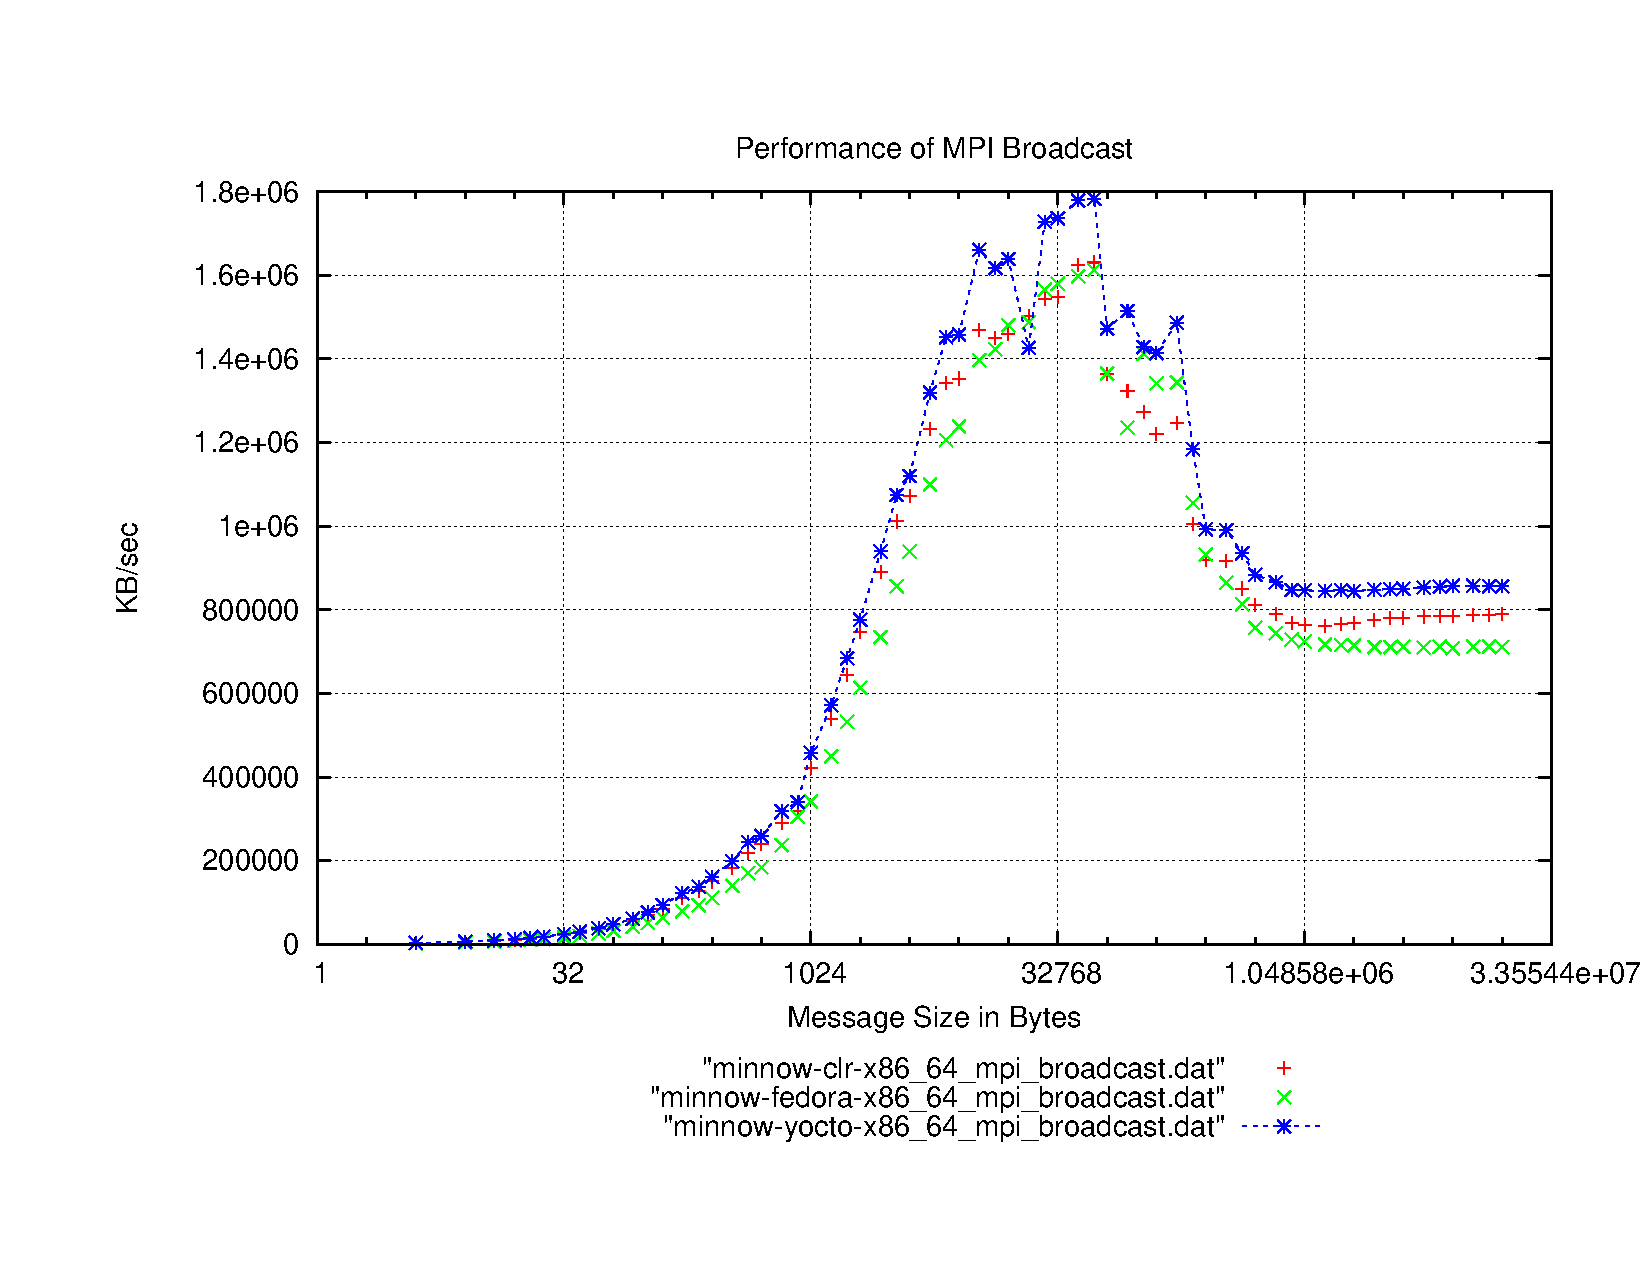
\includegraphics[width=\paperwidth]{images/mpbench_yocto_experiments/mpi_broadcast.pdf}
\caption{\textit{MPI Broadcast} benchmark running in Minnowboard with Clear Linux, Yocto and Fedora }
\label{mpi_broadcast_yocto}
\end{sidewaysfigure}

Based on the results gotten in the previous tests of bi directional band
width (figure \ref{mpi_bibw_clr_fedora}) and the broadcast test (Figure
\ref{mpi_broadcast_clr_fedora}), the main reason why Clear Linux ran with
higher speed was because of the number of processes (forks) since fighting for
the same resources (network / memory / CPU). For this experiment the number of
booting processes in Yocto is 15\% lower than CLR and 35\%
lower than Fedora. This can bee seen in the Figure \ref{number_forks_yocto}.

\begin{figure}[H]
\centering
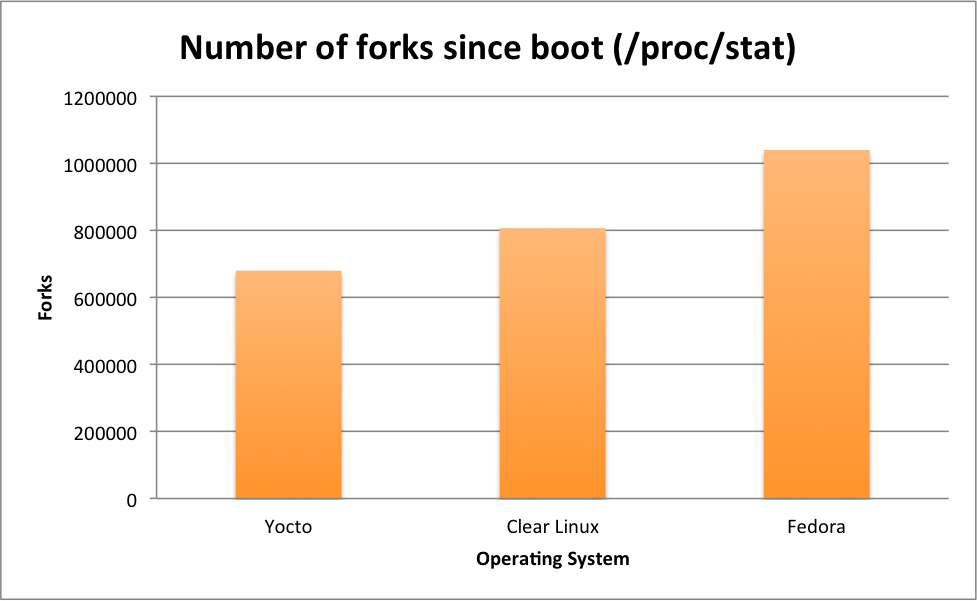
\includegraphics[width=1 \textwidth]{images/number_forks_yocto.png}
\caption{Number of forks since booting process reported in /proc/stat file }
\label{number_forks_yocto}
\end{figure}

Due to the fact that the test are running in a single platform, latency test (Figure
\ref{mpi_latency_yocto} has the same performance despite the change in
operating system.

\begin{sidewaysfigure}
  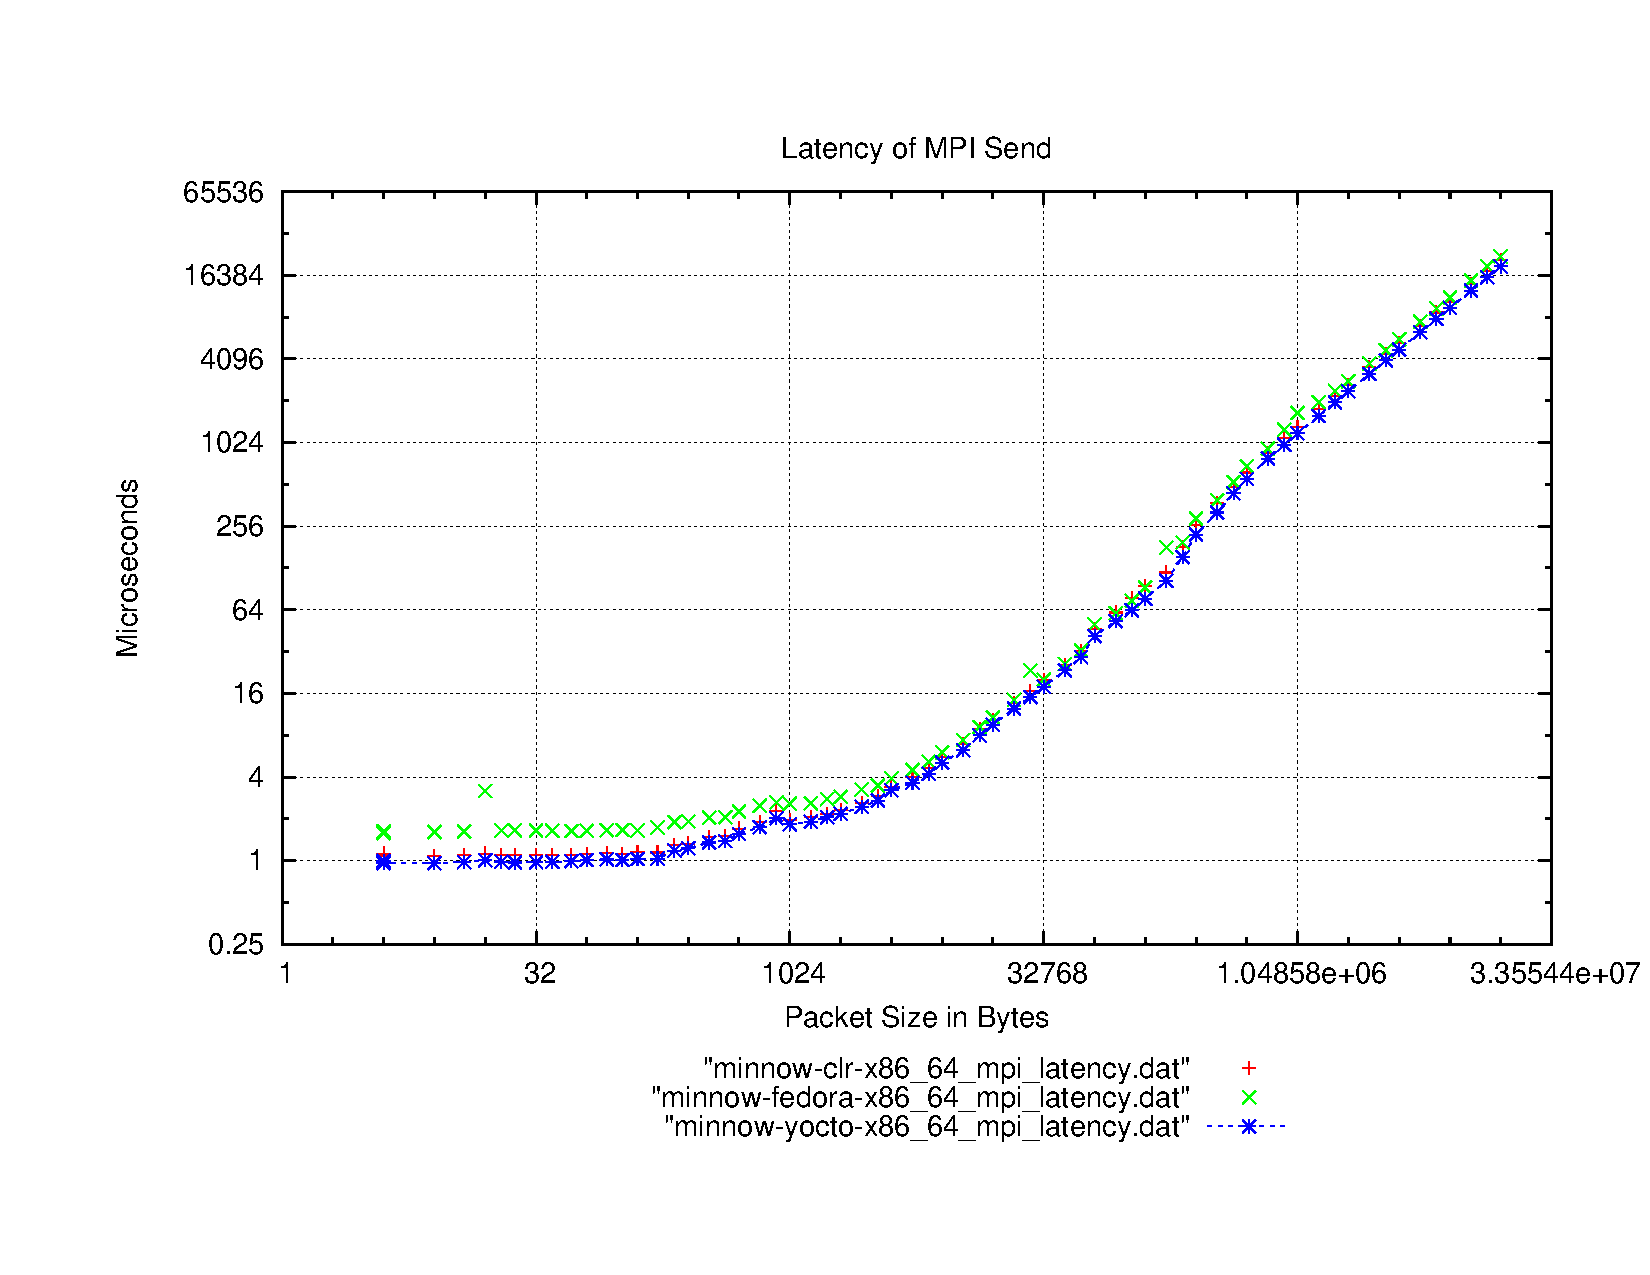
\includegraphics[width=\paperwidth]{images/mpbench_yocto_experiments/mpi_latency.pdf}
\caption{\textit{MPI latency} running in  MinnowBoard MAX  with Clear Linux,
Yocto and Fedora.}
\label{mpi_latency_yocto}
\end{sidewaysfigure}

Figure \ref{mpi_latency_yocto} has similar results than Figure
\ref{mpi_roundtrip_yocto}). Despite the operating system running on the platform
the performance is the same, due to the fact that they were a single platform.


\begin{sidewaysfigure}
  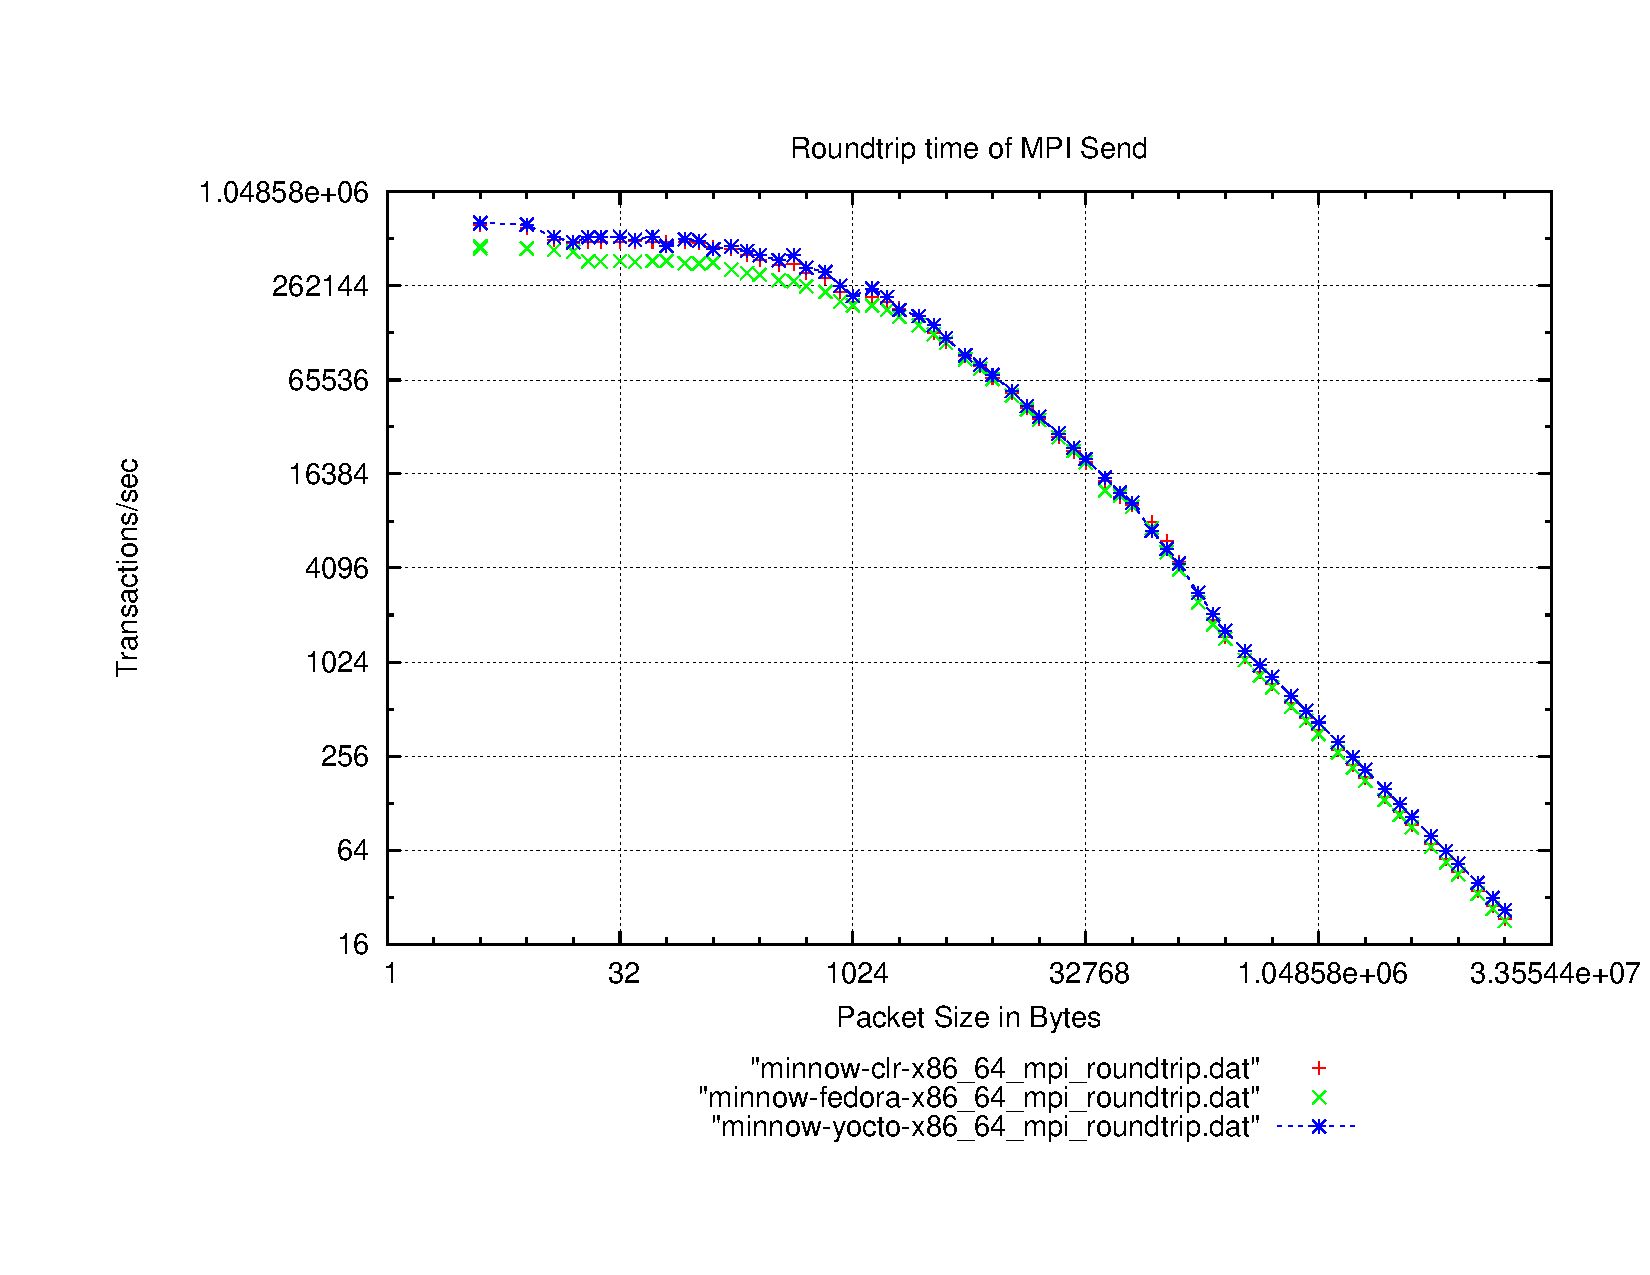
\includegraphics[width=\paperwidth]{images/mpbench_yocto_experiments/mpi_roundtrip.pdf}
\caption{\textit{MPI Bi directional} bandwidth running in  MinnowBoard MAX  with Clear Linux,
Yocto and Fedora.}
\label{mpi_roundtrip_yocto}
\end{sidewaysfigure}

After these experiment is proved that the use of Yocto as the operating system
for the embedded platforms improves the performance of the MPI benchmarks. 

\section{MPI Benchmark Performance Comparison Between Cluster of Embedded
Systems and a Desktop Computing System}

The system under test (Hardware and Software) for this experiment is described
in the Table~\ref{tab:mpi_perf_comp}
    
    \begin{minipage}{\textwidth}
    \end{minipage}

    \begin{center}
    \begin{tabular}{ | l | r |}
        \hline
        \textbf{Platform under test} & \shortstack{MinnowBoard MAX and \\  Intel  NUC D54250WYK } \\ \hline
        \textbf{Number of embedded platforms}  & 6  \\ \hline
        \textbf{Number of desktop platforms}  & 1  \\ \hline
        \textbf{Operating System on embedded platform} & Yocto  \\ \hline
        \textbf{Operating System on desktop platform} & Clear Linux  \\ \hline
    \end{tabular}
    \captionof{table}{Description of system under test (HW/SW) for MPI
    benchmark performance comparison between cluster of embedded
    systems and a desktop computing system}\label{tab:mpi_perf_comp}
    \end{center}

After doing the experiments in a single Atom-based system it was  decided to do the
experiments in a cluster of them. The experiment is limited to the number of
available systems we can gather. In this case, it was possible to get six  MinnowBoard MAX
platforms \cite{minnowboard} platforms to do the experiments. The full diagram
of the cluster is described below in Figure \ref{fig:4.4}.

All these systems execute the MPIBenchmarks with the following ssh config file:

\begin{minipage}{\textwidth}
\end{minipage}

\begin{minipage}{\textwidth}

\begin{lstlisting}[frame=single]
  $ cat ~/.ssh/config
    Host node1
        HostName node1-ip-or-hostname
        User user-of-the-ssh-key
        Port port-if-nedded

    Host node2
        HostName node1-ip-or-hostname
        User user-of-the-ssh-key
        Port port-if-nedded

    Host node3
        HostName node1-ip-or-hostname
        User user-of-the-ssh-key
        Port port-if-nedded

\end{lstlisting}

\end{minipage}

And the following MPI config file:

\begin{minipage}{\textwidth}
\end{minipage}

\begin{minipage}{\textwidth}
\begin{lstlisting}[frame=single]
  $ cat hostfile
    node1
    node2
    node3
\end{lstlisting}

\end{minipage}

This is necessary to make the systems communicate each other through MPI , if
we don't include this configuration there will not be any communications due to
the fact that MPI requires an ssh connection. 

The idea of this experiment is to compare the performance of the cluster of
embedded systems to a traditional computing system (NUC D54250WYK \cite{NUC}).
In this case, the desktop system is based on the processor i5-4250U CPU. The
main components of that system is described in Chapter 4 (Table \ref{tab:4.2}).

\subsection{Results}

After executing the MPI benchmark in the cluster of embedded systems  and in
the NUC D54250WYK \cite{NUC} (with Clear Linux OS \cite{clear-linux}) their
comparison results are shown in following figures. 


\begin{sidewaysfigure}
  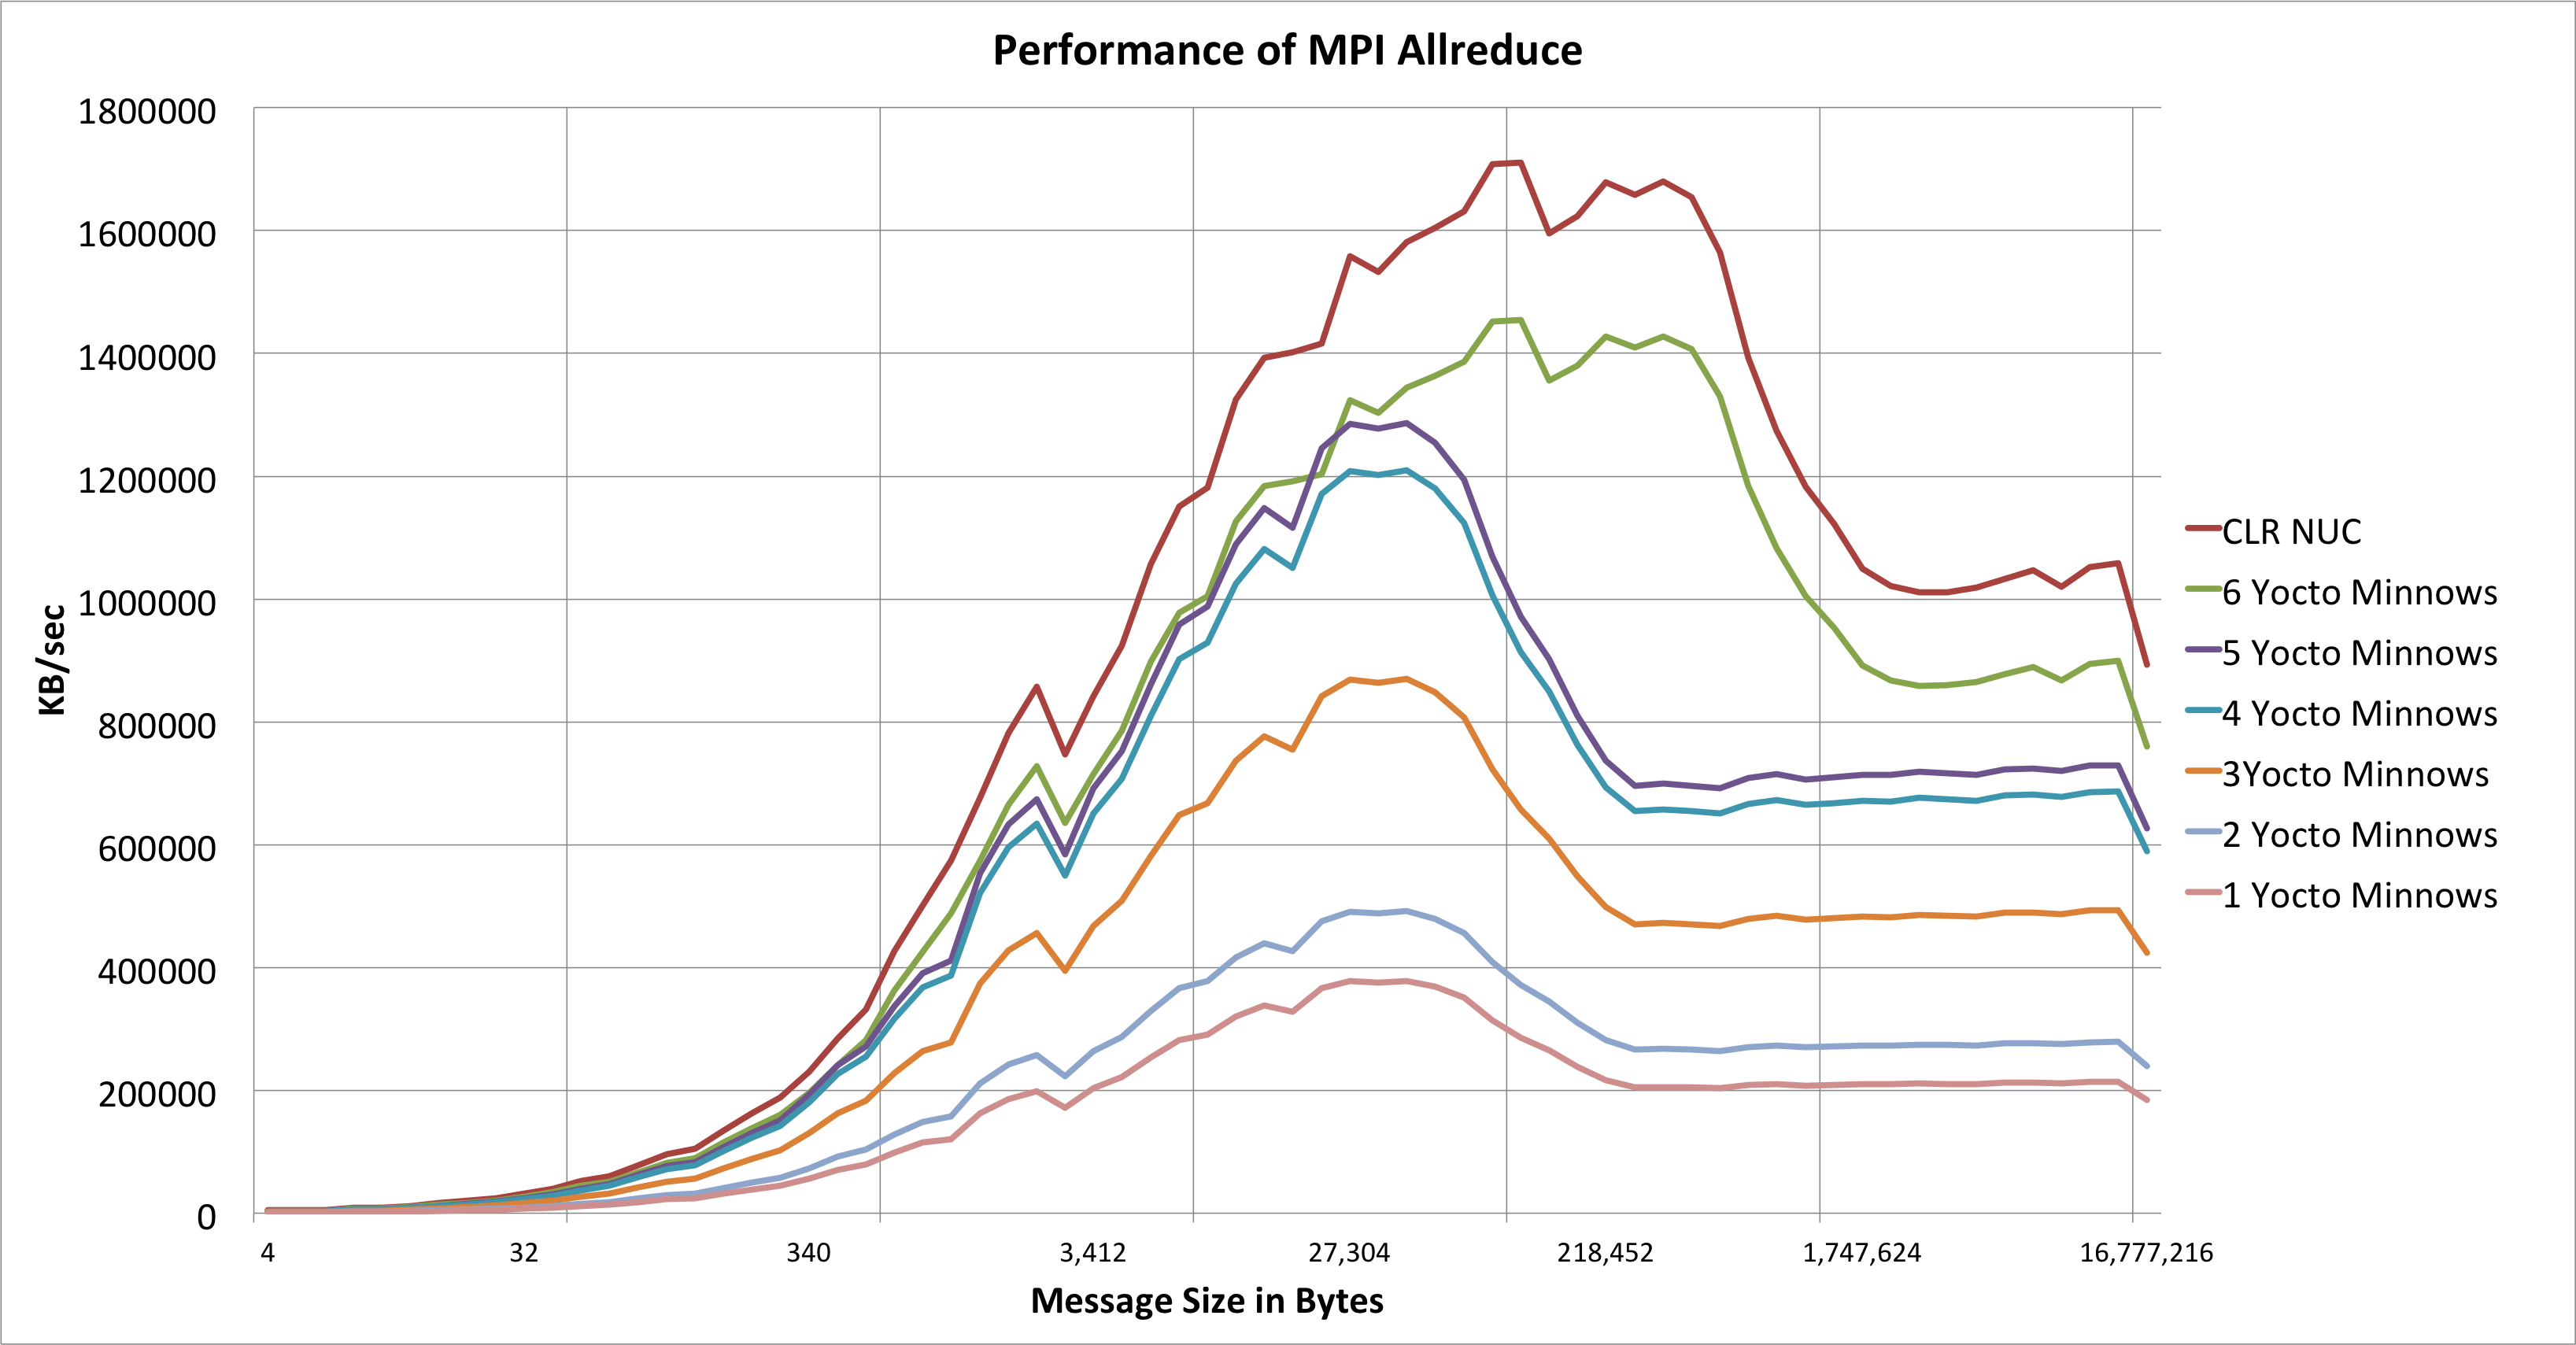
\includegraphics[width=\paperwidth]{images/mpbench_cluster_experiments/mpi_all_reduce.png}
\caption{\textit{Allreduce} benchmark in cluster of embedded platforms with Yocto OS and NUC
with Clear Linux OS.}
\label{all_reduce_cluster}
\end{sidewaysfigure}

The \textit{all reduce} benchmark starts to have a gain in performance with the
addition of more embedded platforms into the cluster of embedded platforms.
With two platforms the gain is not seen; however, with three or more the gain is
substantial.  When the system has five or four platforms it has similar
performance. With six platforms the performance is similar (even in the drop
point) that the desktop platform \cite{NUC}

\begin{sidewaysfigure}
  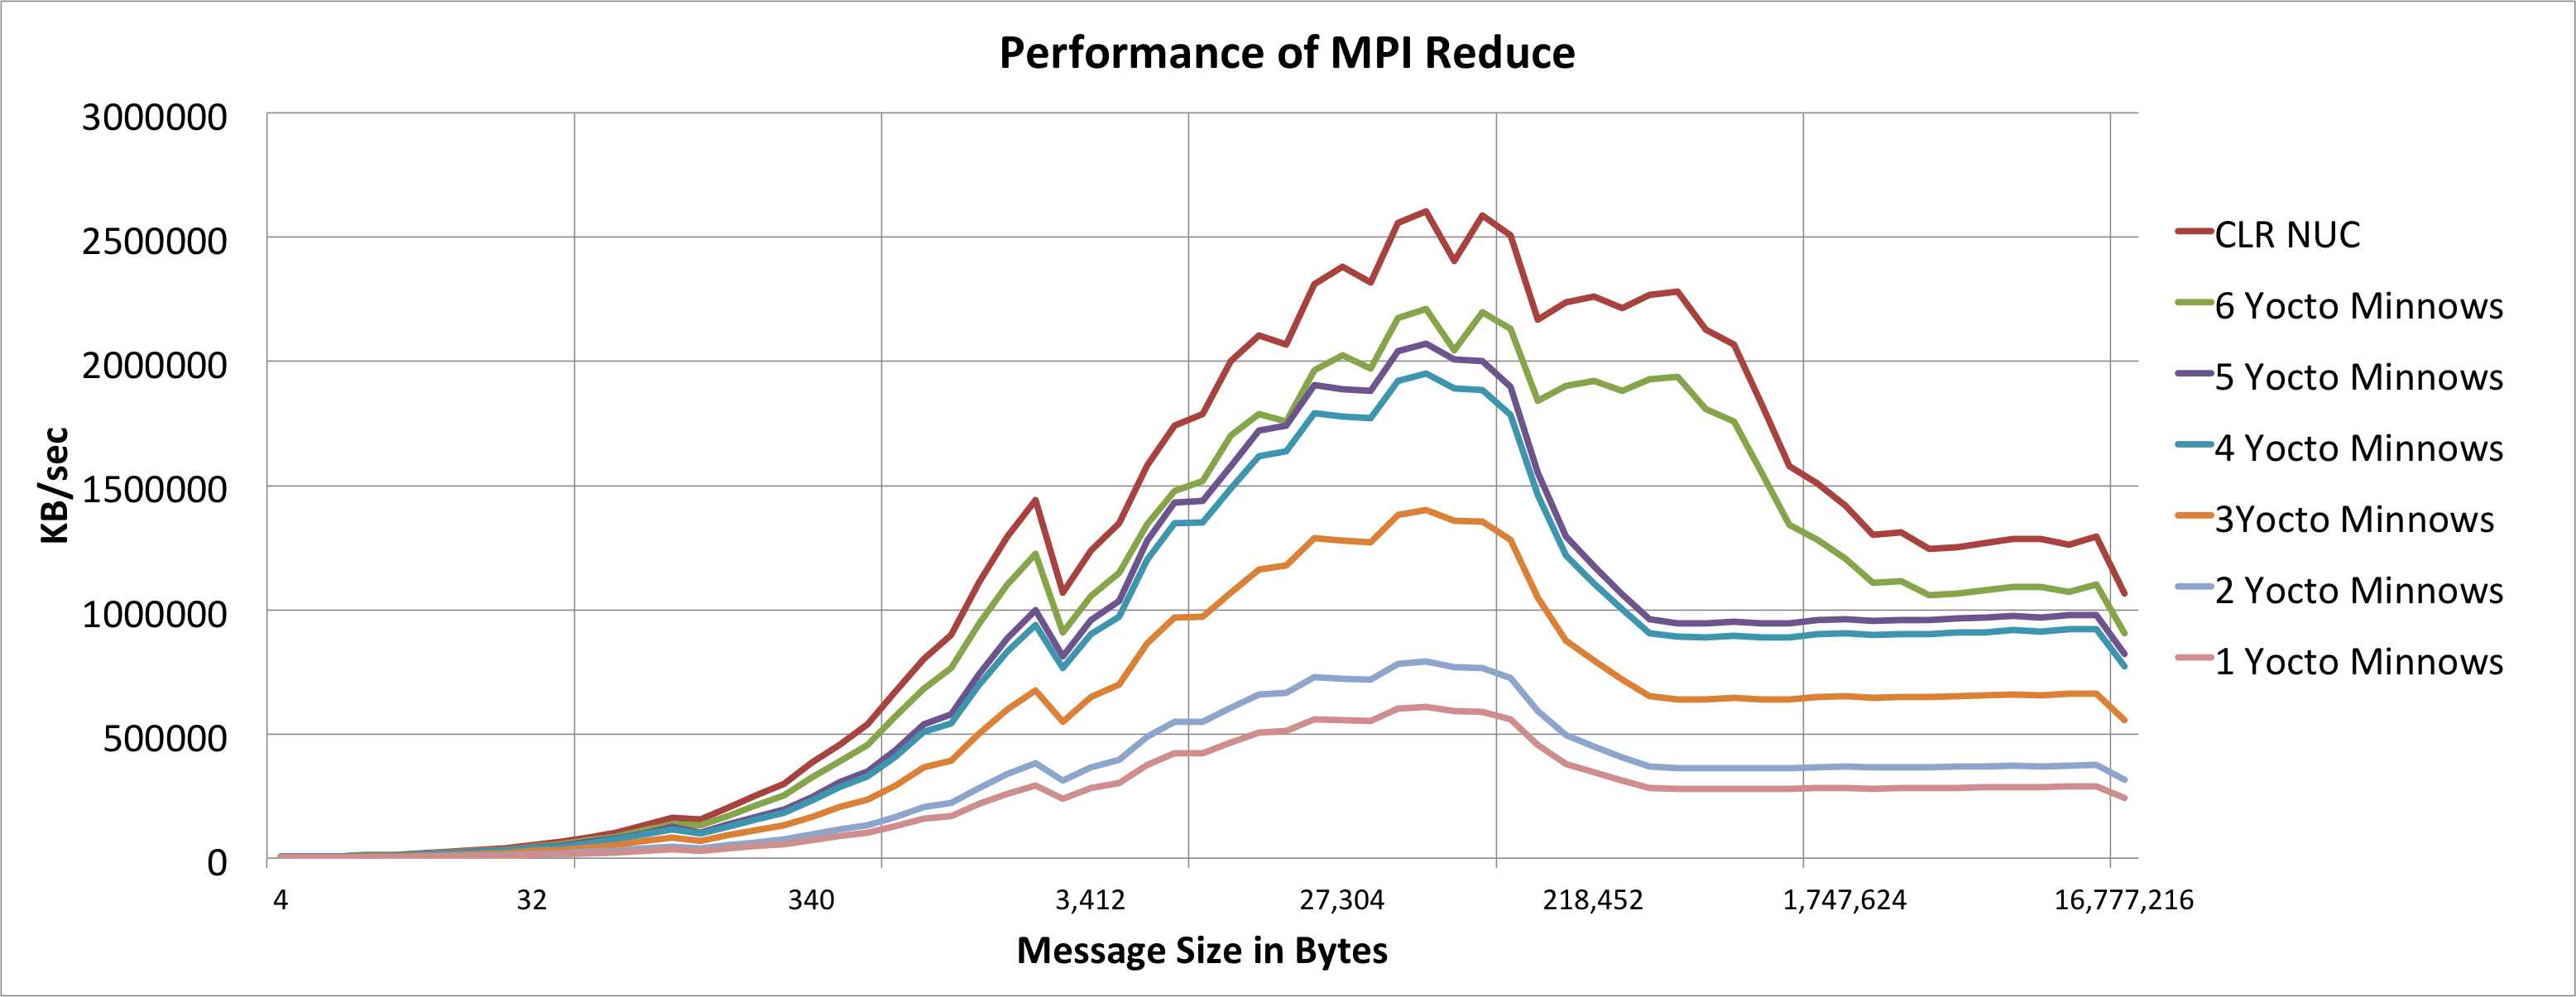
\includegraphics[width=\paperwidth]{images/mpbench_cluster_experiments/mpi_reduce.png}
\caption{\textit{Reduce} benchmark in cluster of embedded platforms with Yocto OS and NUC
with Clear Linux OS.}
\label{reduce_cluster}
\end{sidewaysfigure}

In the \textit{reduce} benchmark the performance is constant across the
increment of platforms in the cluster of embedded platforms. Even the similar
performance that three and four platforms present.

\begin{sidewaysfigure}
  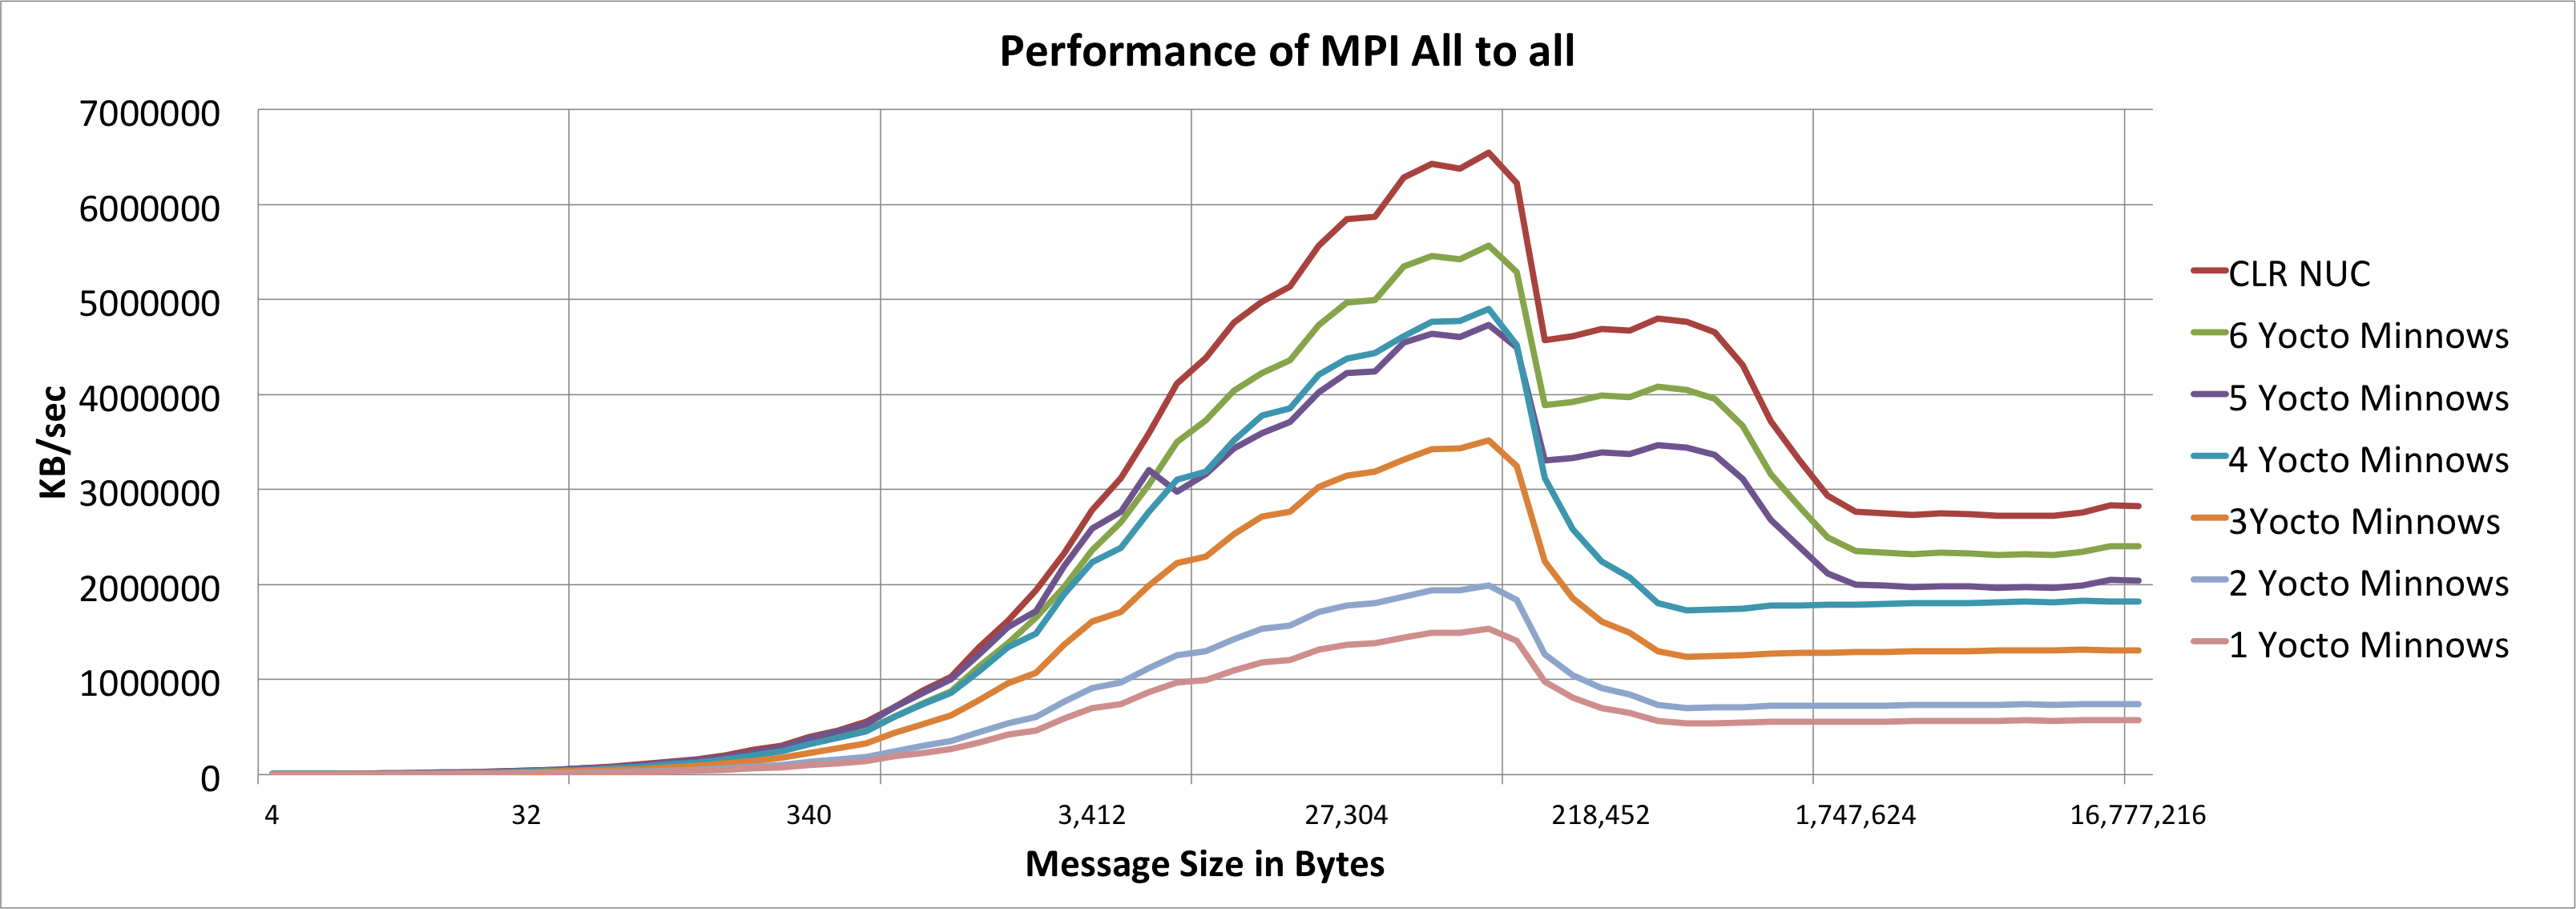
\includegraphics[width=\paperwidth]{images/mpbench_cluster_experiments/mpi_alltoall.png}
\caption{\textit{All to All} benchmark in cluster of embedded platforms with Yocto OS and NUC
with Clear Linux OS.}
\label{all_to_all_cluster}
\end{sidewaysfigure}

In the \textit{All to all} benchmark presented in
Figure\ref{all_to_all_cluster} the performance at 218MB is similar despite the
number of platforms the cluster has. In this test the performance of even six
platforms is not close to the performance that a NUC \cite{NUC} system can has.

\begin{sidewaysfigure}
  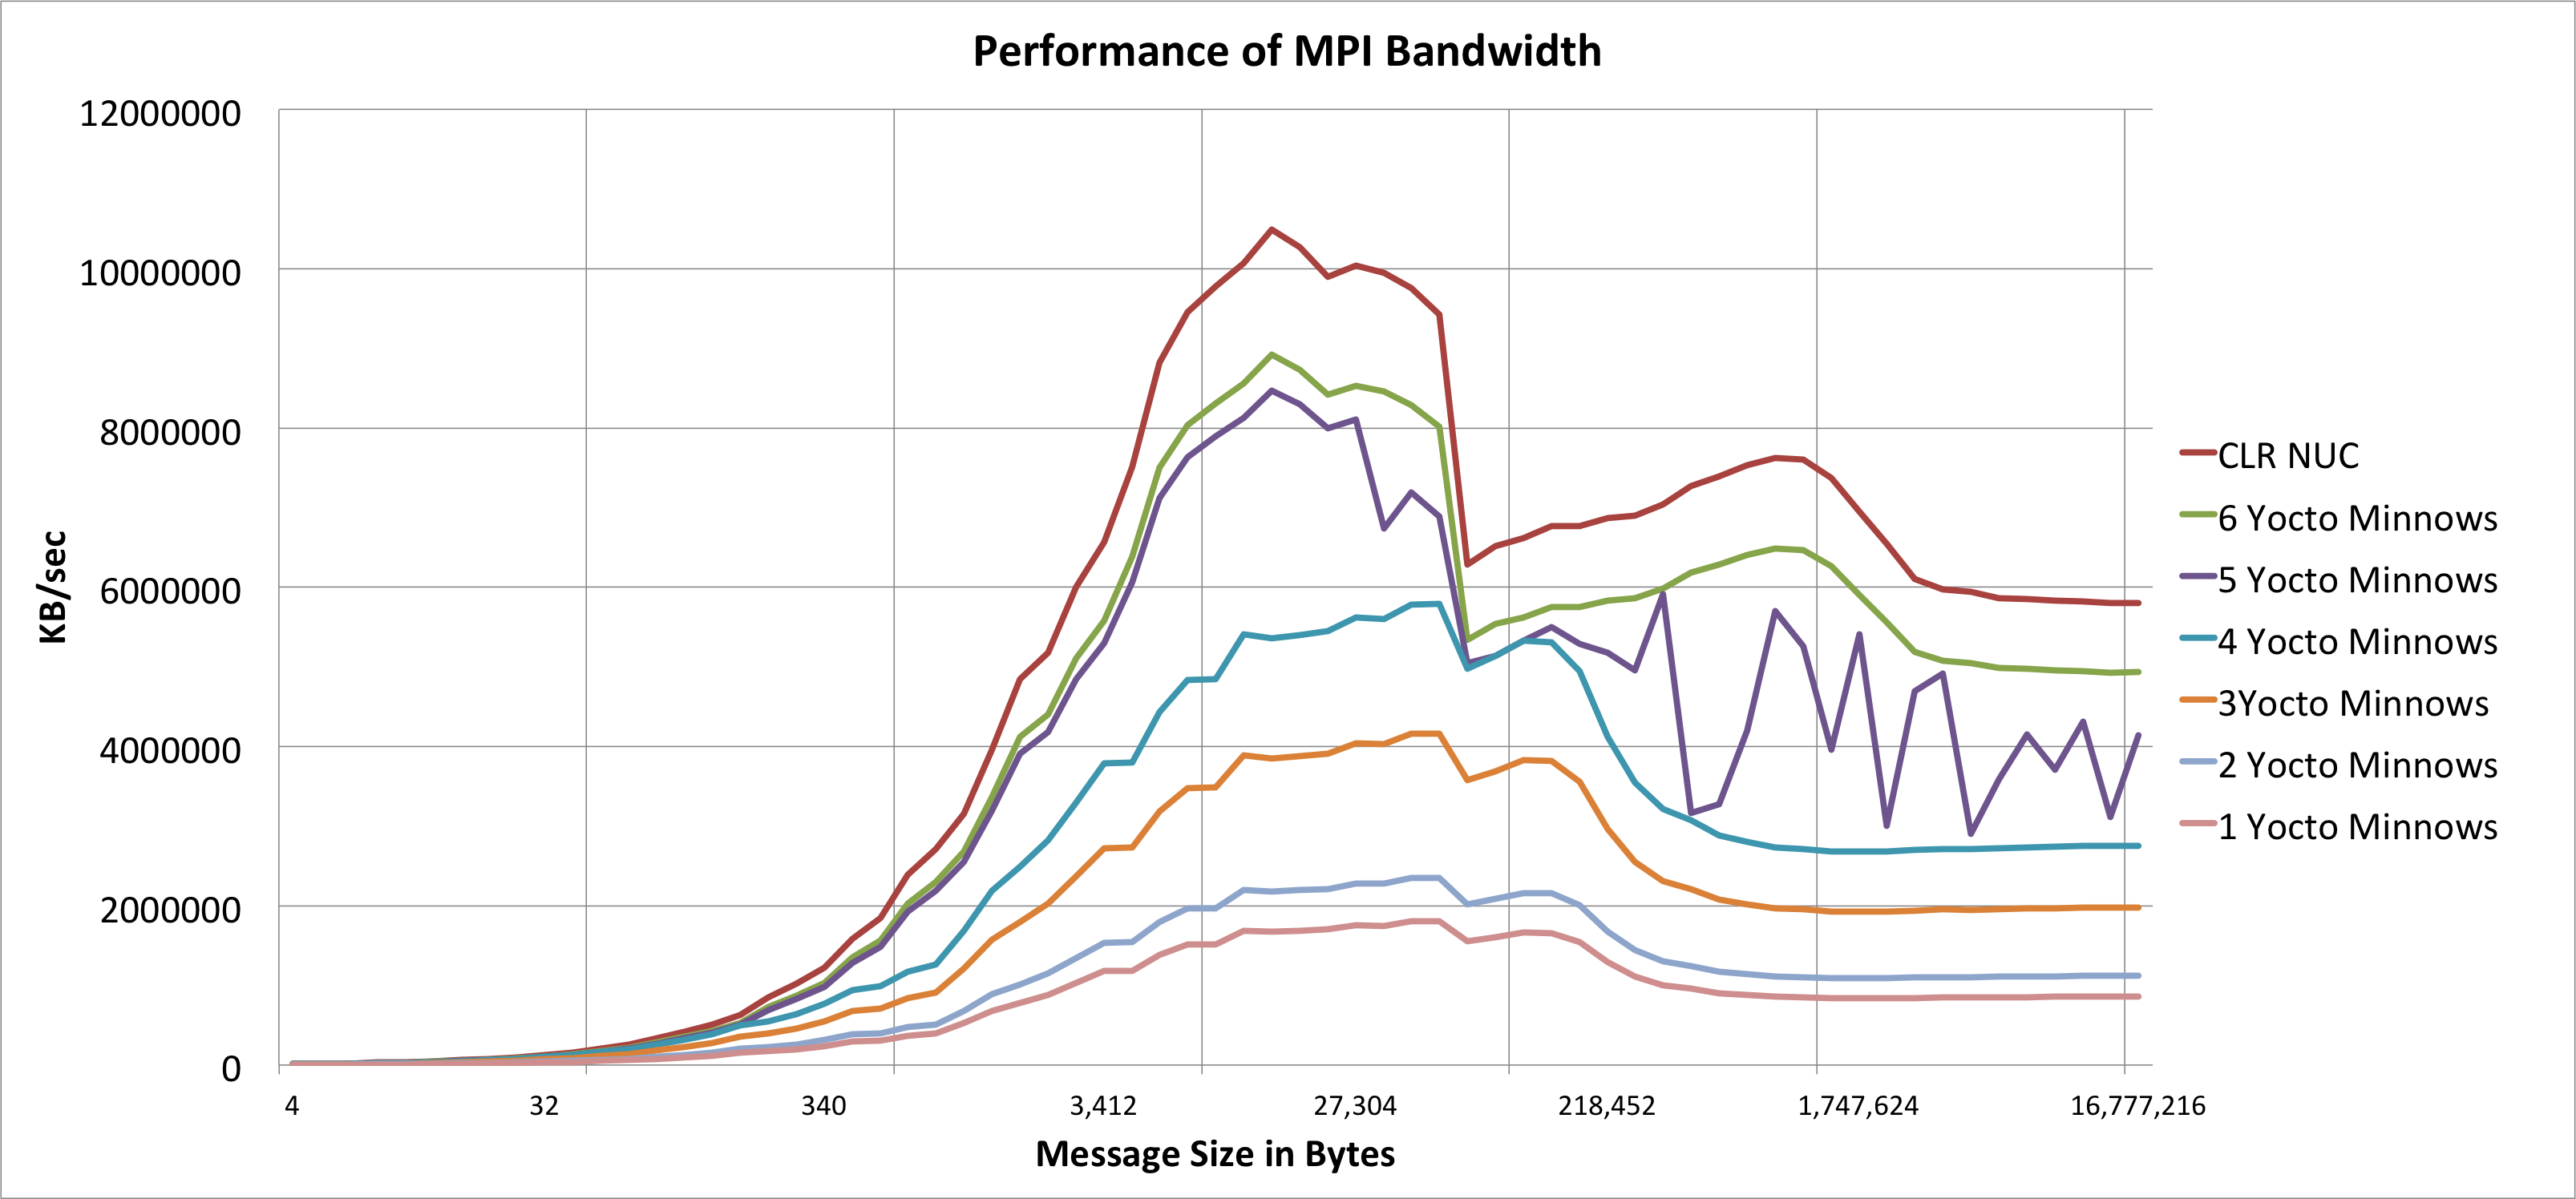
\includegraphics[width=\paperwidth]{images/mpbench_cluster_experiments/mpi_bandwidth.png}
\caption{\textit{Bandwidth} benchmark in cluster of embedded platforms with Yocto OS and NUC
with Clear Linux OS.}
\label{bandwidth_cluster}
\end{sidewaysfigure}

In the \textit{Bandwidth} performance test it can be seen an interesting
behaivor with a cluster of 5 MinnowBoard MAX systems (Figure
\ref{bandwidth_cluster}). At 218 MB the performance became unstable. The
performance can be similar to the one presented by four or 6 platforms. Besides
that the performance with other number of platforms is similar to the one
presented in Figure \ref{all_to_all_cluster}.  Even the fact that the
performance at 218MB is similar despite the number of platforms the cluster
has.

\begin{sidewaysfigure}
  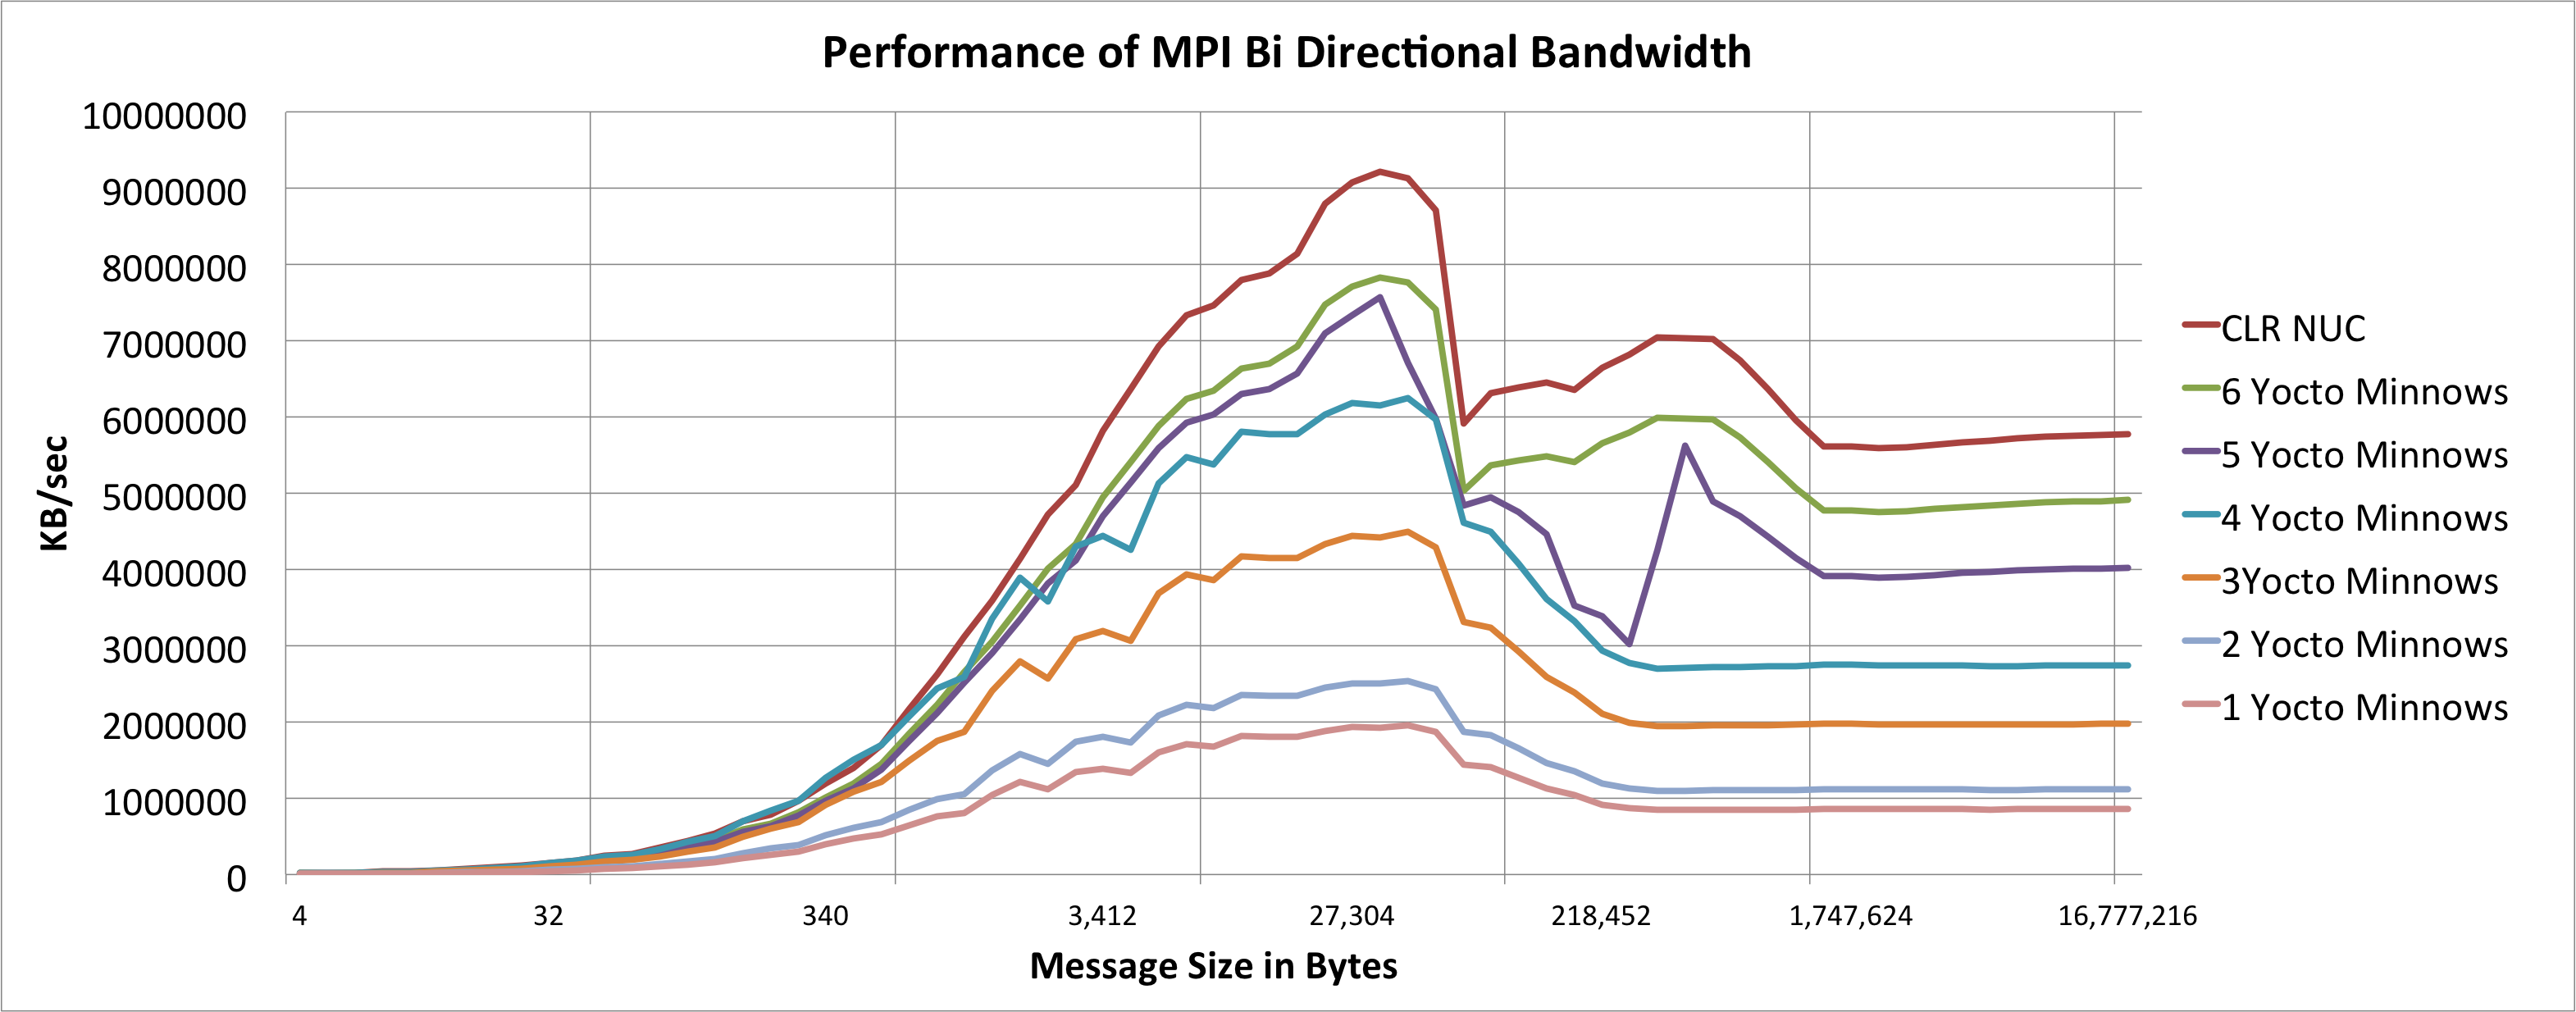
\includegraphics[width=\paperwidth]{images/mpbench_cluster_experiments/mpi_bibw.png}
\caption{\textit{Bi directional bandwidth} benchmark in cluster of embedded platforms with Yocto OS and NUC
with Clear Linux OS.}
\label{bibw_cluster}
\end{sidewaysfigure}

In the \textit{Bi directional bandwidth} benchmark in Figure \ref{bibw_cluster}
a similar behavior than in Figure \ref{bandwidth_cluster}.  At 218 MB the
performance became unstable, with similar performance from four, five and six
platforms. Besides that the increment in performance is constant. Even with
three or four platforms the performance improvement is high. From these results
it can be seen that for applications that requires speeds between 27MB and
218MB, a cluster of four, five or six embedded platforms can bring similar
performance that a traditional desktop system, in terms of bi directional
bandwidth.

\begin{sidewaysfigure}
  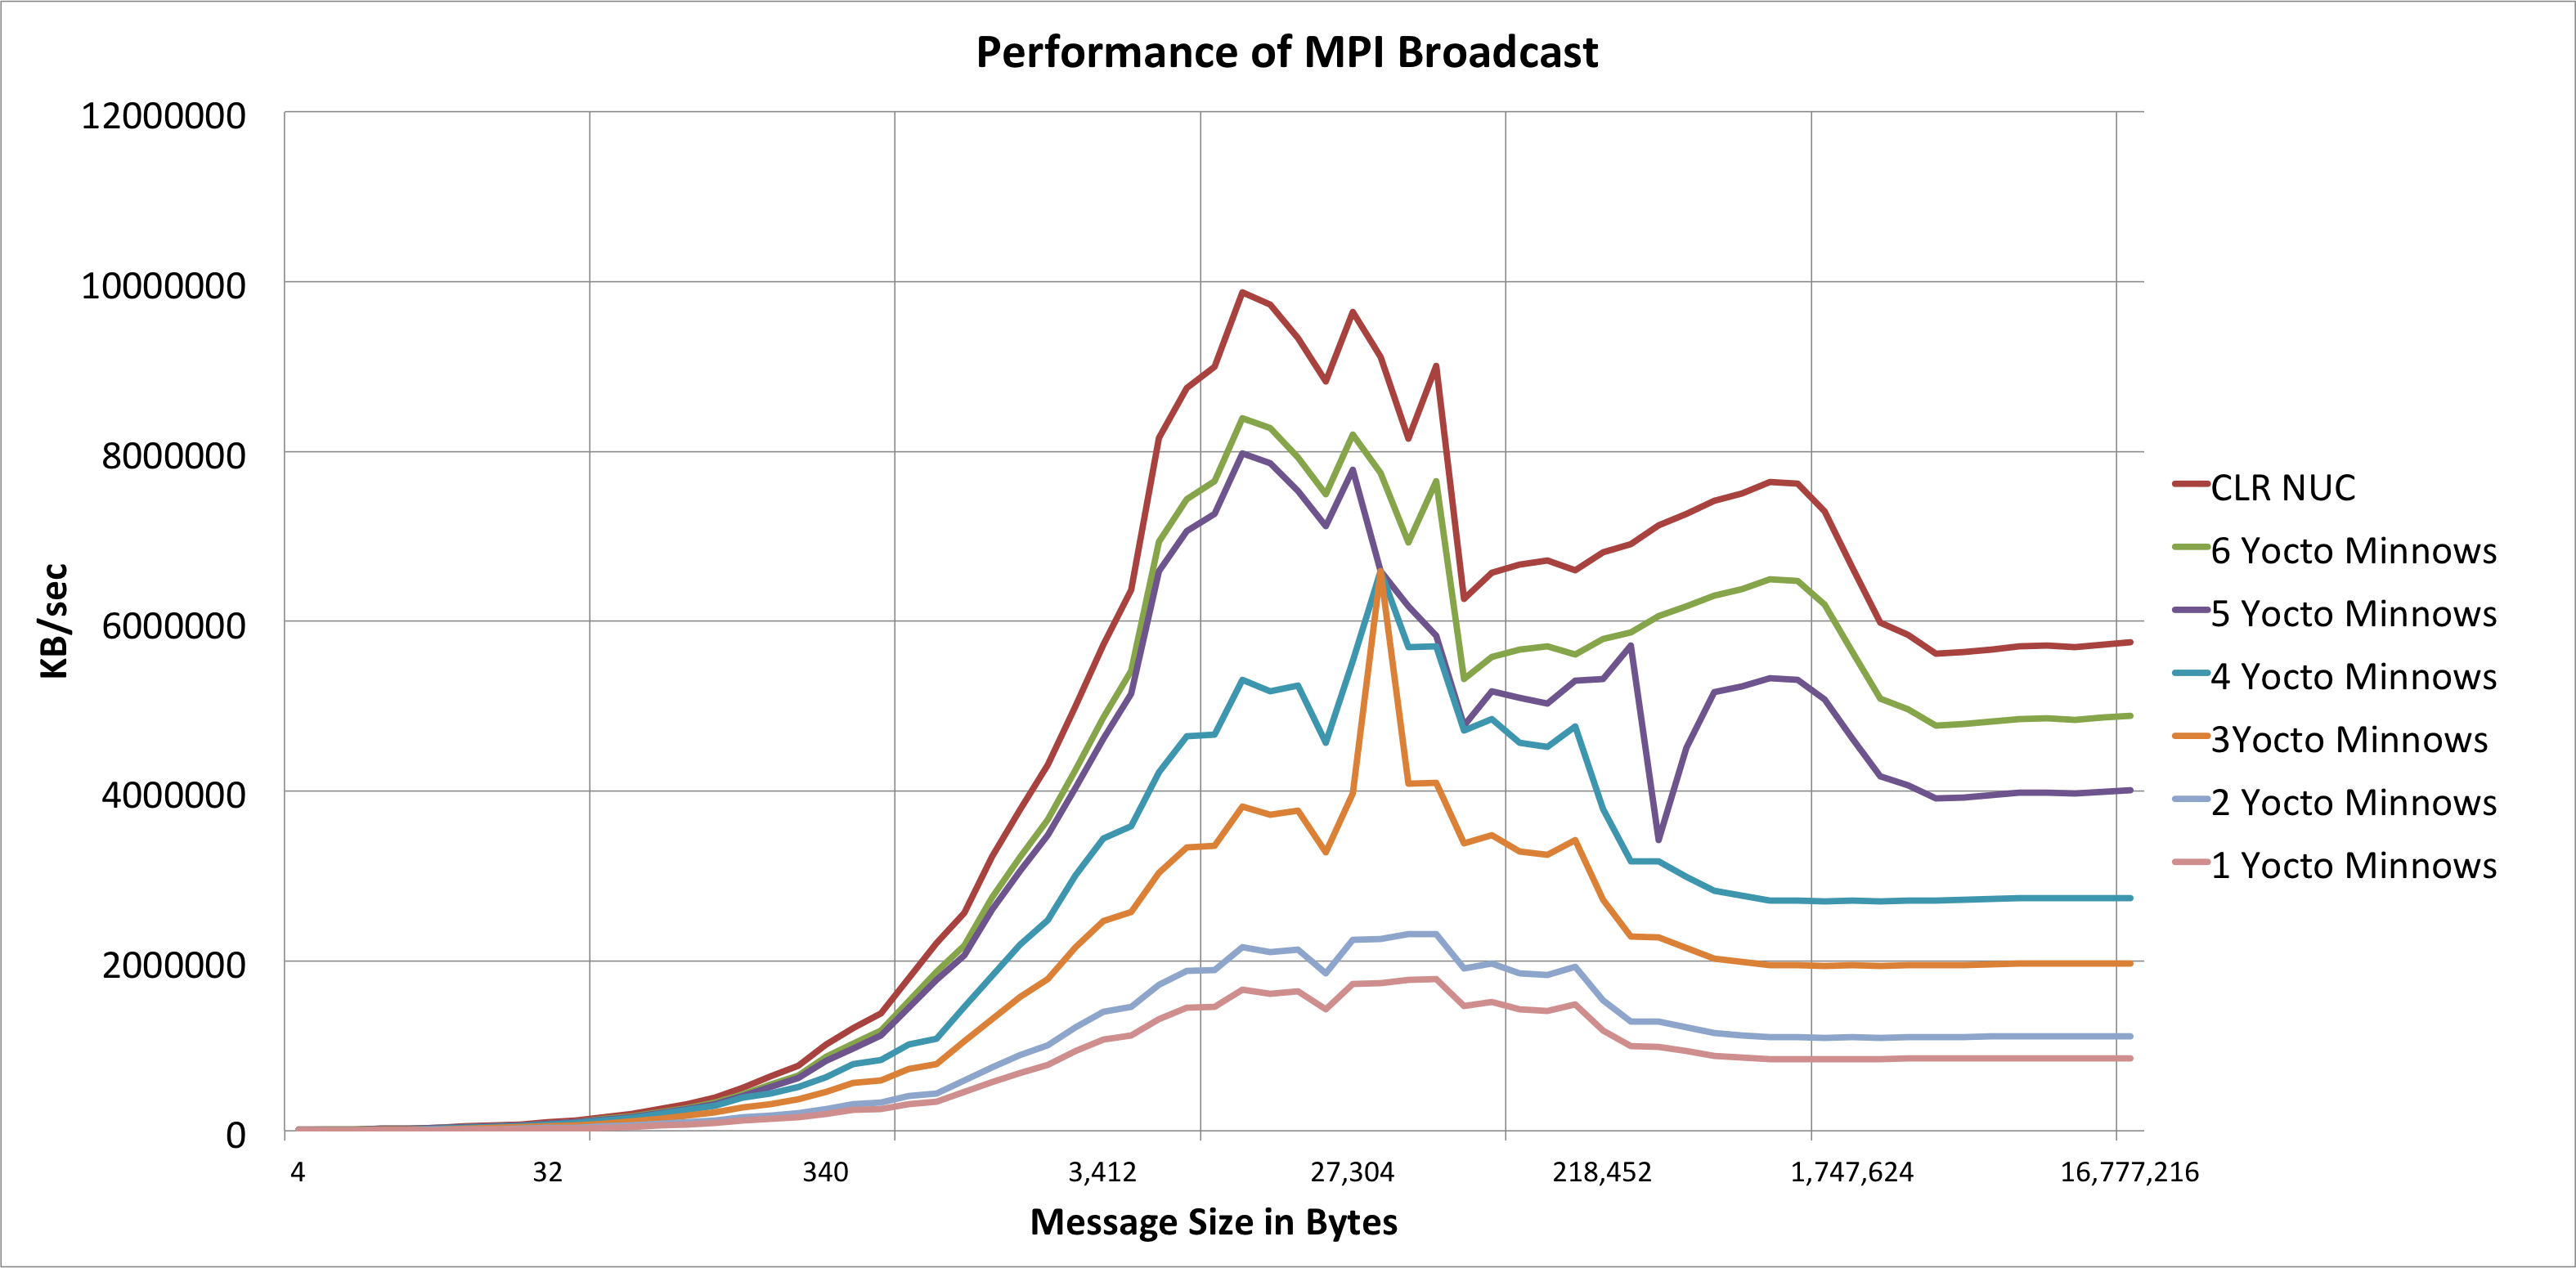
\includegraphics[width=\paperwidth]{images/mpbench_cluster_experiments/mpi_broadcast.png}
\caption{\textit{Broadcast} benchmark in cluster of embedded platforms with Yocto OS and NUC
with Clear Linux OS.}
\label{broadcast_cluster}
\end{sidewaysfigure}

The \textit{Broadcast} benchmark in cluster of embedded platforms with Yocto OS
presents similar performance with three, four, five or six platforms. In this
case the fluctuation of performance among these configurations starts 27MB
until 1,7 GB.

\begin{sidewaysfigure}
  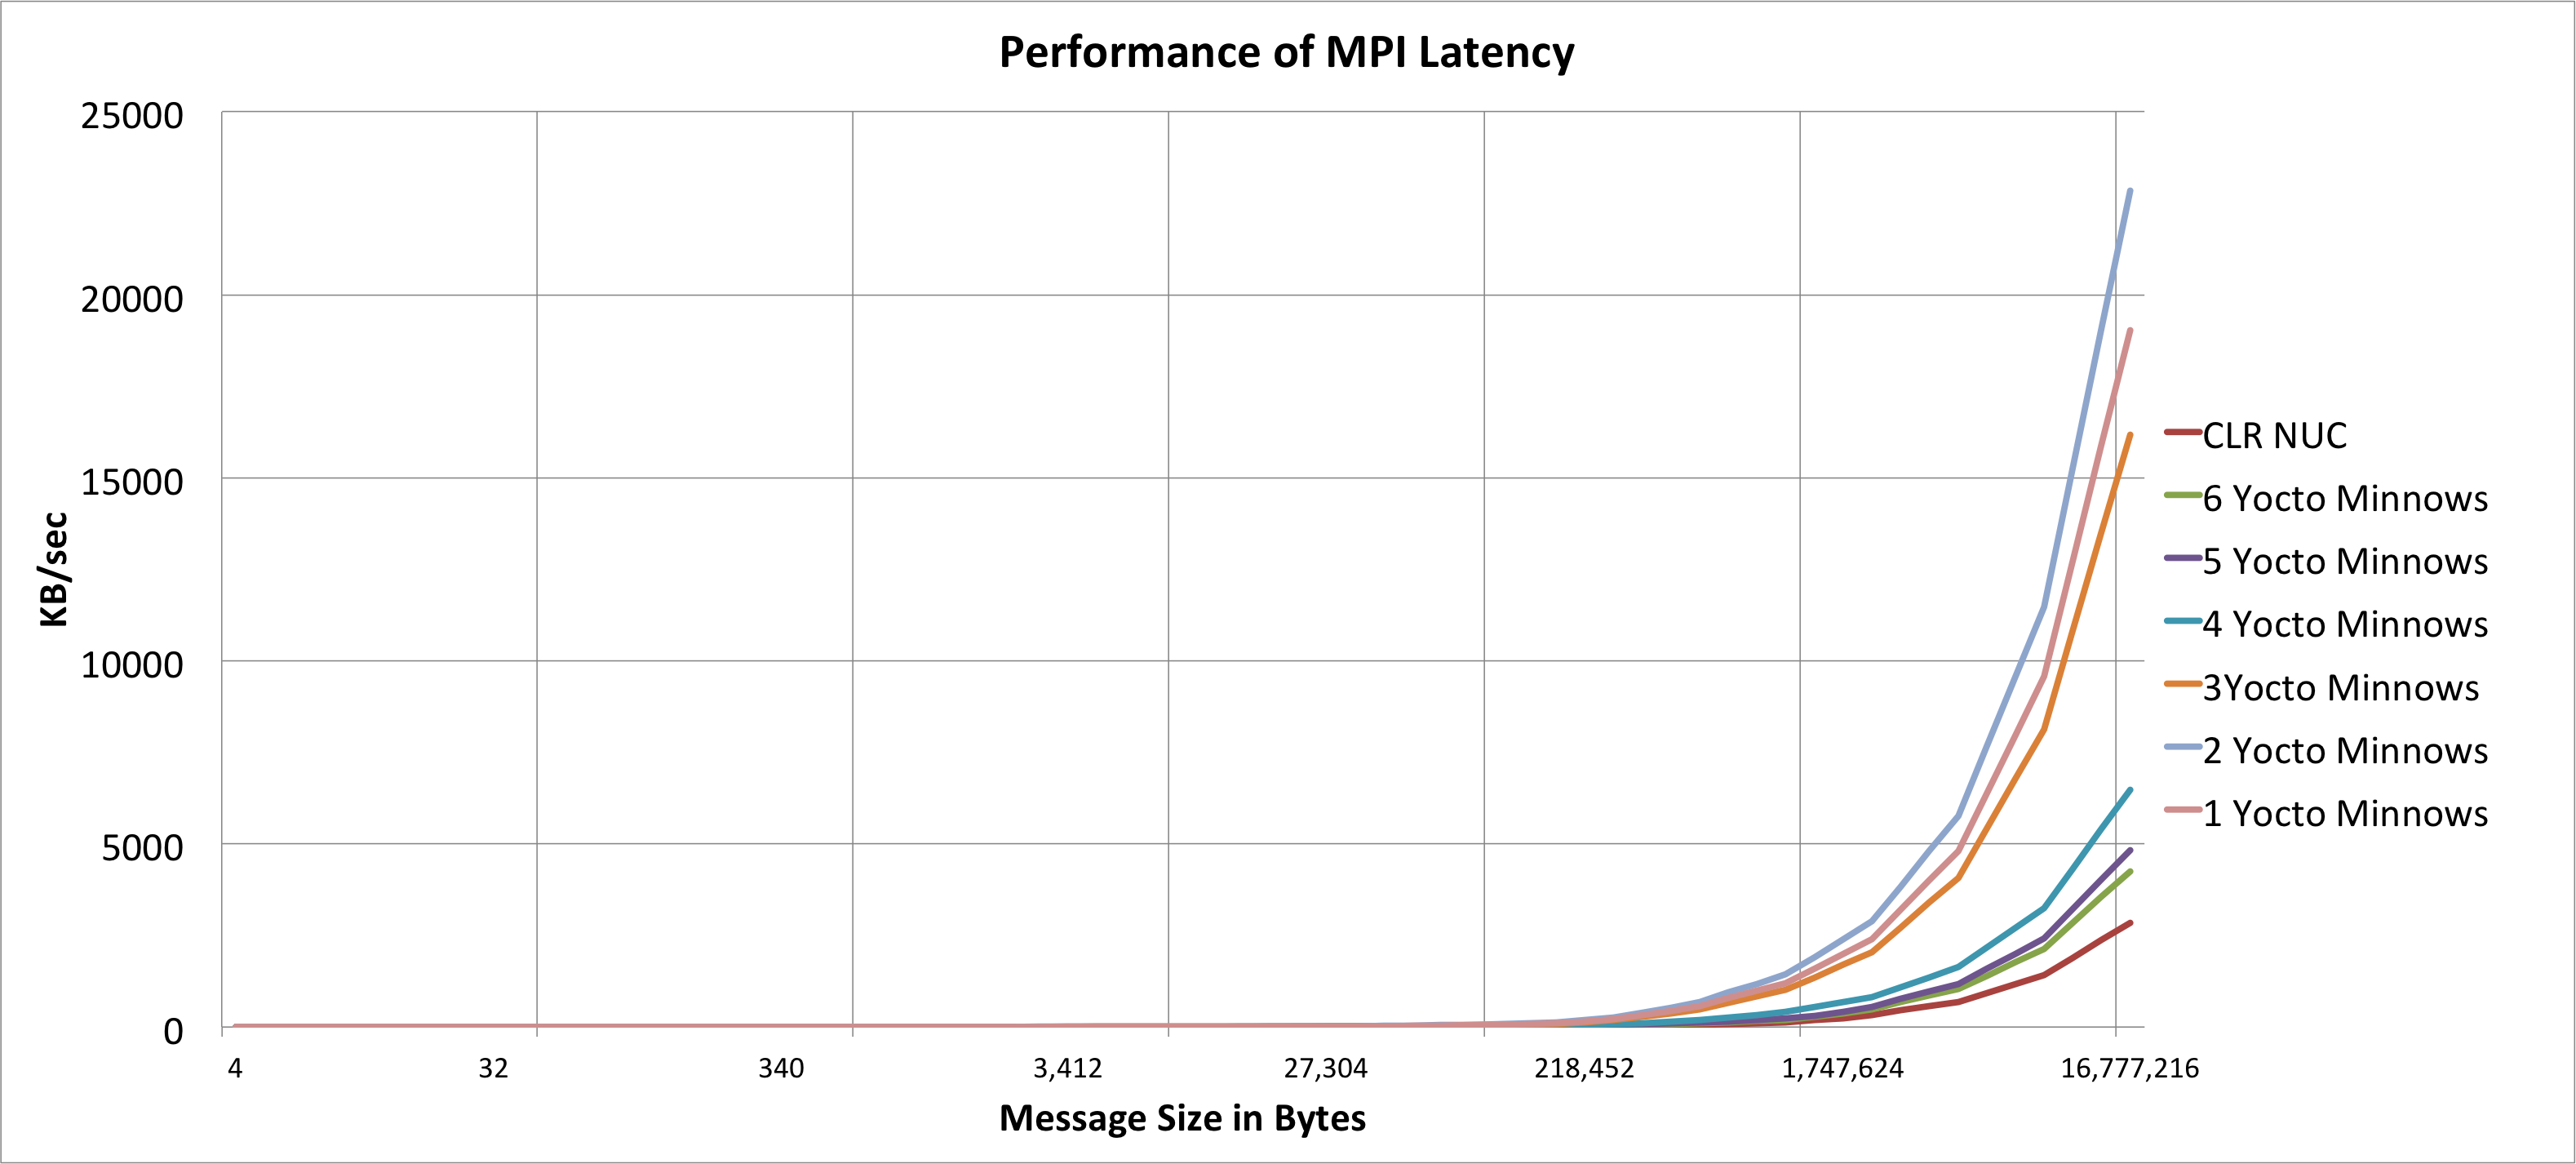
\includegraphics[width=\paperwidth]{images/mpbench_cluster_experiments/mpi_latency.png}
\caption{\textit{Latency} benchmark in cluster of embedded platforms with Yocto OS and NUC
with Clear Linux OS.}
\label{latency_cluster}
\end{sidewaysfigure}

Latency is higher (Figure \ref{latency_cluster} and Figure
\ref{roundtrip_cluster})in the cluster of embedded platforms.  This is a side
effect of the distributed systems.  Total latency is a combination of both
hardware and software factors, with the software contribution generally being
much greater than that of the hardware. Latency is really important when the
program is dominated by communication, and the messages are small.  This can
happen when scaling to larger numbers of nodes. In the experiments we perform we
can see that the latency of the cluster of embedded platforms is high in
comparison to the centralized system \cite{NUC} 

\begin{sidewaysfigure}
  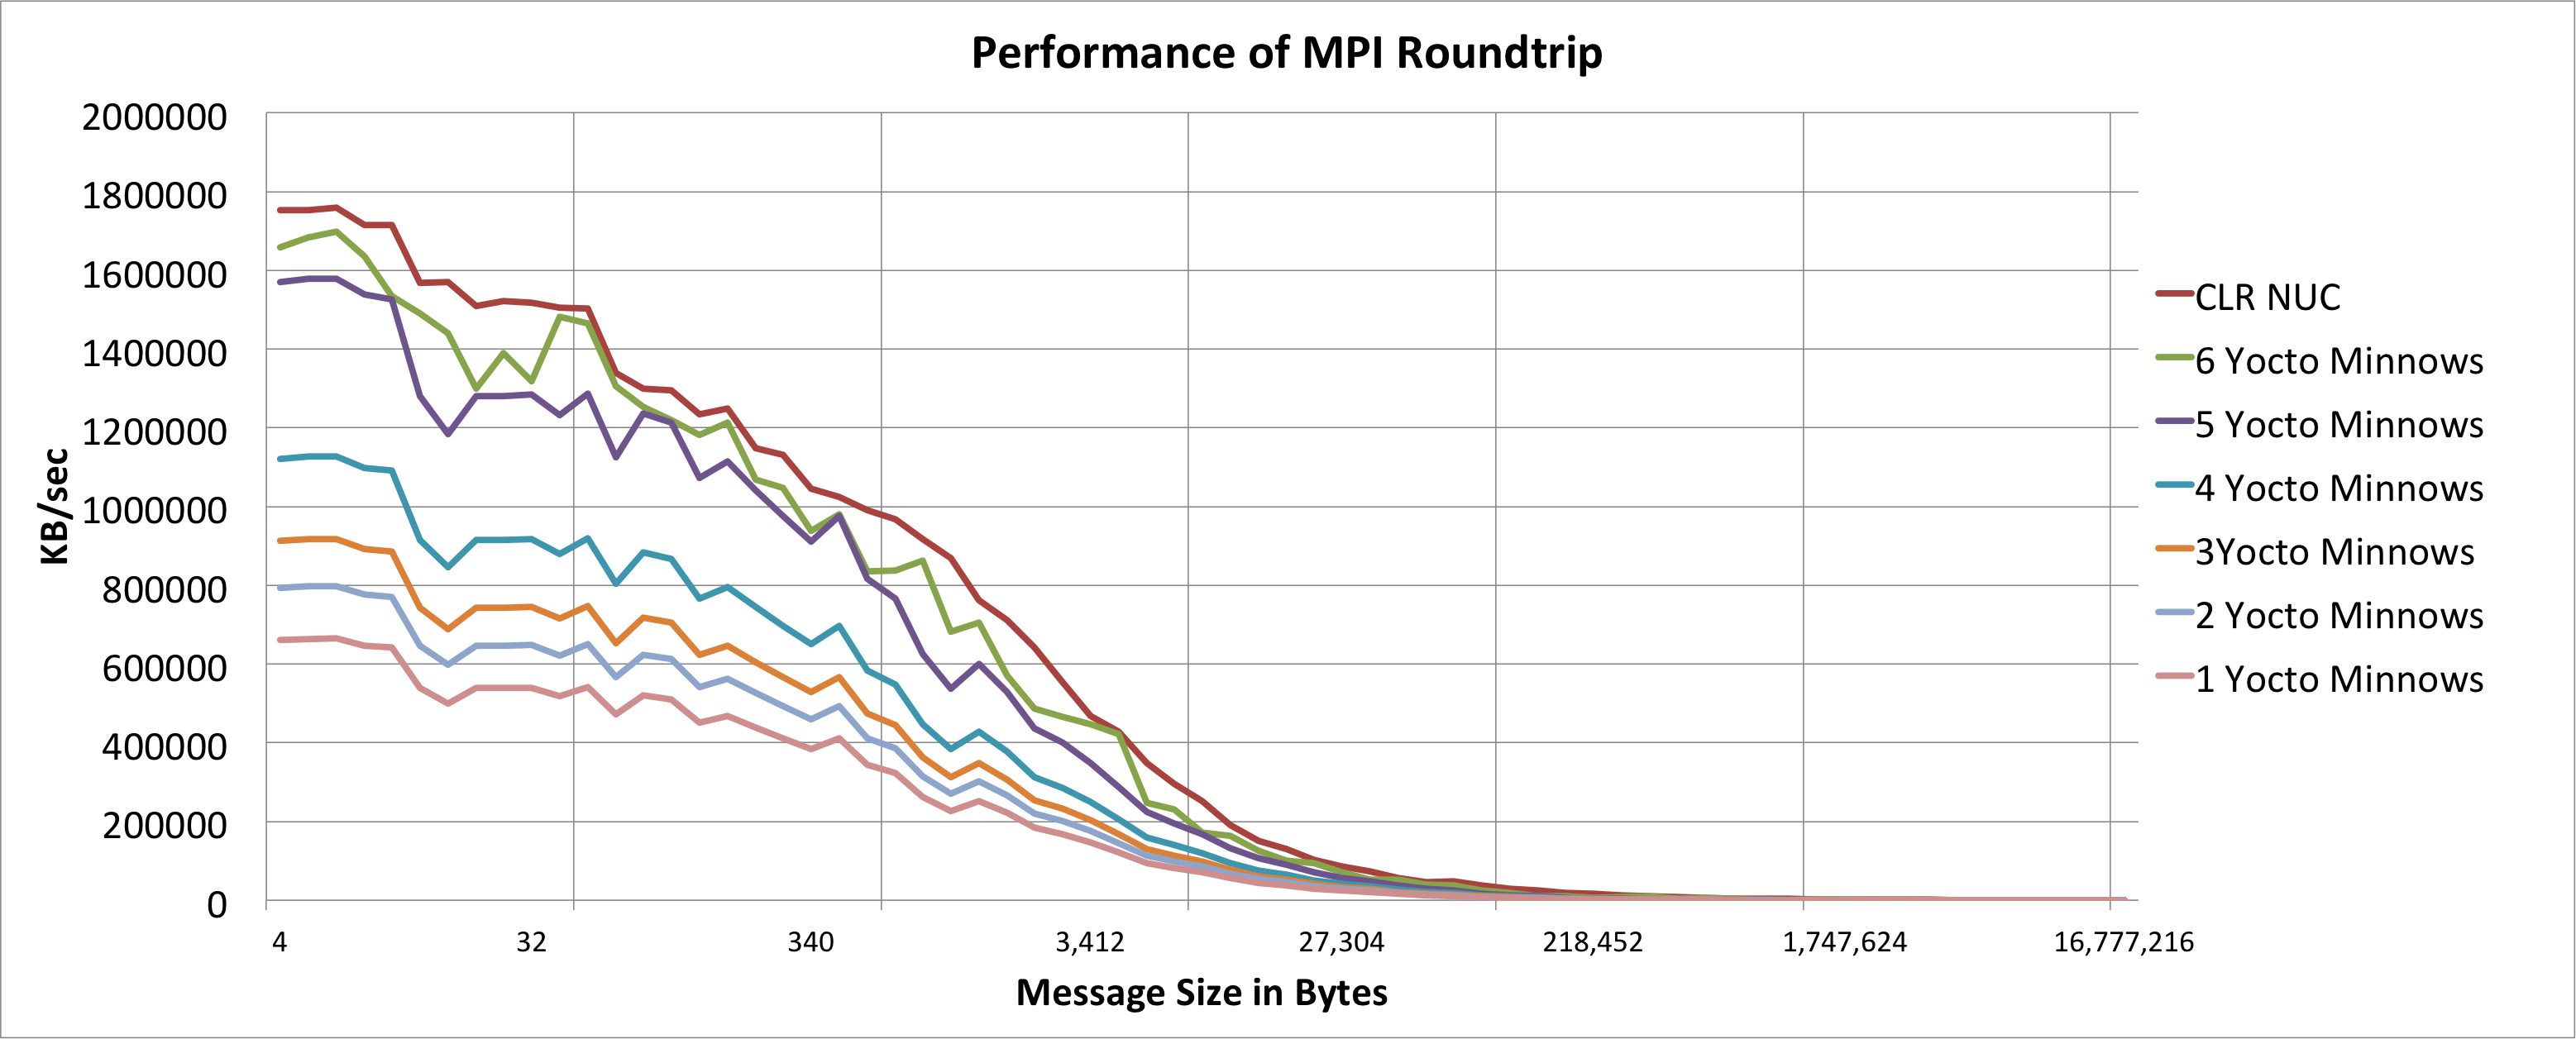
\includegraphics[width=\paperwidth]{images/mpbench_cluster_experiments/mpi_roundtrip.png}
\caption{\textit{Roundtrip} benchmark in cluster of embedded platforms with Yocto OS and NUC
with Clear Linux OS.}
\label{roundtrip_cluster}
\end{sidewaysfigure}

\section{Power Efficiency Comparison of Cluster of Embedded Systems to a
Desktop Computing System}

It has been described that for six systems of embedded platform it is not
possible to get the same performance impact that with desktop computing
systems.So far we have been able to see the performance comparison of a traditional
computer system and a cluster of embedded systems, only up to 85\% of the
performance for some tests. The hypothesis of this work is to determine the
optimal point at which it is better to send data to a server instead of
performing local computations.


According to the hypothesis of this work, the expected behavior of power
efficiency for the cluster of embedded systems is represented in
Figure~\ref{fig:1.2}. In the beginning the increment on the
number of nodes in the network will increment the performance (top part of
on equation \ref{eq:5}), but at the same time the amount of watts will
increase making the energy efficiency flat at some point (if the lower part of
the equation increases then energy efficiency tends to decrease).

The next natural step is to measure the power consumption of both systems : the
cluster of embedded systems and the D54250WYK.

The instrument to measure the power consumption of the system is the WT300
Series Digital Power Meter (from Yokogawa) . Digital Power Analyzers are
instruments for laboratory, manufacturing test, or embedded applications to
accurately measure and analyze electrical power characteristics.

Table \ref{minnow_power_1} describes the power consumption of a single
MinnowBoard MAX.

\begin{table}[]
    \centering
    \resizebox{\textwidth}{!}{
    \begin{tabular}{|l|l|l|l|l|l|l|l|l|}
    \hline
          &All reduce &Reduce & All to all &Bandwidht & Bi direct bandwidth & Boradcast & Latency & Roundtrip \\ \hline 
          Average Power Consumption (Watts) & 4.234  & 2.231 & 2.876 & 4.9871 & 4.7865 & 4.8721  & 4.1235  & 4.8563 \\ \hline
          MAX Watts & 5.6139 & 5.875 & 5.934 & 5.823 & 5.749  & 5.853 & 5.761 & 5.703 \\ \hline
          MIN Watts & 2.8874 & 2.234 & 2.7532 & 2.8342 & 2.7431  & 2.6548 & 2.934  & 2.985 \\ \hline
          Average Power at idle (Watts) & 2.5663 & 2.5663 & 2.5663 & 2.5663 & 2.5663 & 2.5663 & 2.5663  & 2.5663 \\ \hline
    \end{tabular}}
    \captionof{table}{Power consumption of Minnow Board Max with MPI benchmarking}
    \label{minnow_power_1}
\end{table}


The Table \ref{NUC_power_1} describe the power consumption of a single NUC
D54250WYK.


\begin{table}[]
    \centering
    \resizebox{\textwidth}{!}{
    \begin{tabular}{|l|l|l|l|l|l|l|l|l|}
    \hline
          & All reduce & Reduce  & All to all &
          Bandwidht & Bi directional bandwidth &
          Boradcast & Latency & Roundtrip \\ \hline
          Average Power Consumption (Watts) &
          18.0742    & 19.2853 & 18.6589    &
          18.2385   & 18.8423                  &
          19.4739   & 18.8664 & 19.6473   \\ \hline
          MAX Watts                         &
          20.3010    & 20.1011 & 20.4240    &
          20.8761   & 19.9573                  &
          20.8436   & 20.3242 & 20.3452   \\ \hline
          MIN Watts                         &
          5.2046     & 4.4239  & 5.9853     &
          6.5838    & 5.4086                   &
          4.5973    & 6.2199  & 6.8419    \\ \hline
          Average Power at idle (Watts)     &
          4.4801     & 4.4801  & 4.4801     &
          4.4801    & 4.4801                   &
          4.4801    & 4.4801  & 4.4801    \\ \hline
        \end{tabular}}
    \caption{Power consumption of NUC D54250WYK with MPI benchmarking}
    \label{NUC_power_1}
\end{table}


It is seen that the average power consumption of the NUC is close to 20 watts in
the meantime the average power consumption of the embedded system is close to
2 Watts. This is due to the design of the embedded system, just the CPU in the
embedded system is designed to consume 1 watt in idle mode.

Next it was measured the power consumption of the embedded cluster,
this can bee seen in Figure \ref{power_average_minnow}: 

\begin{figure}[H]
\centering
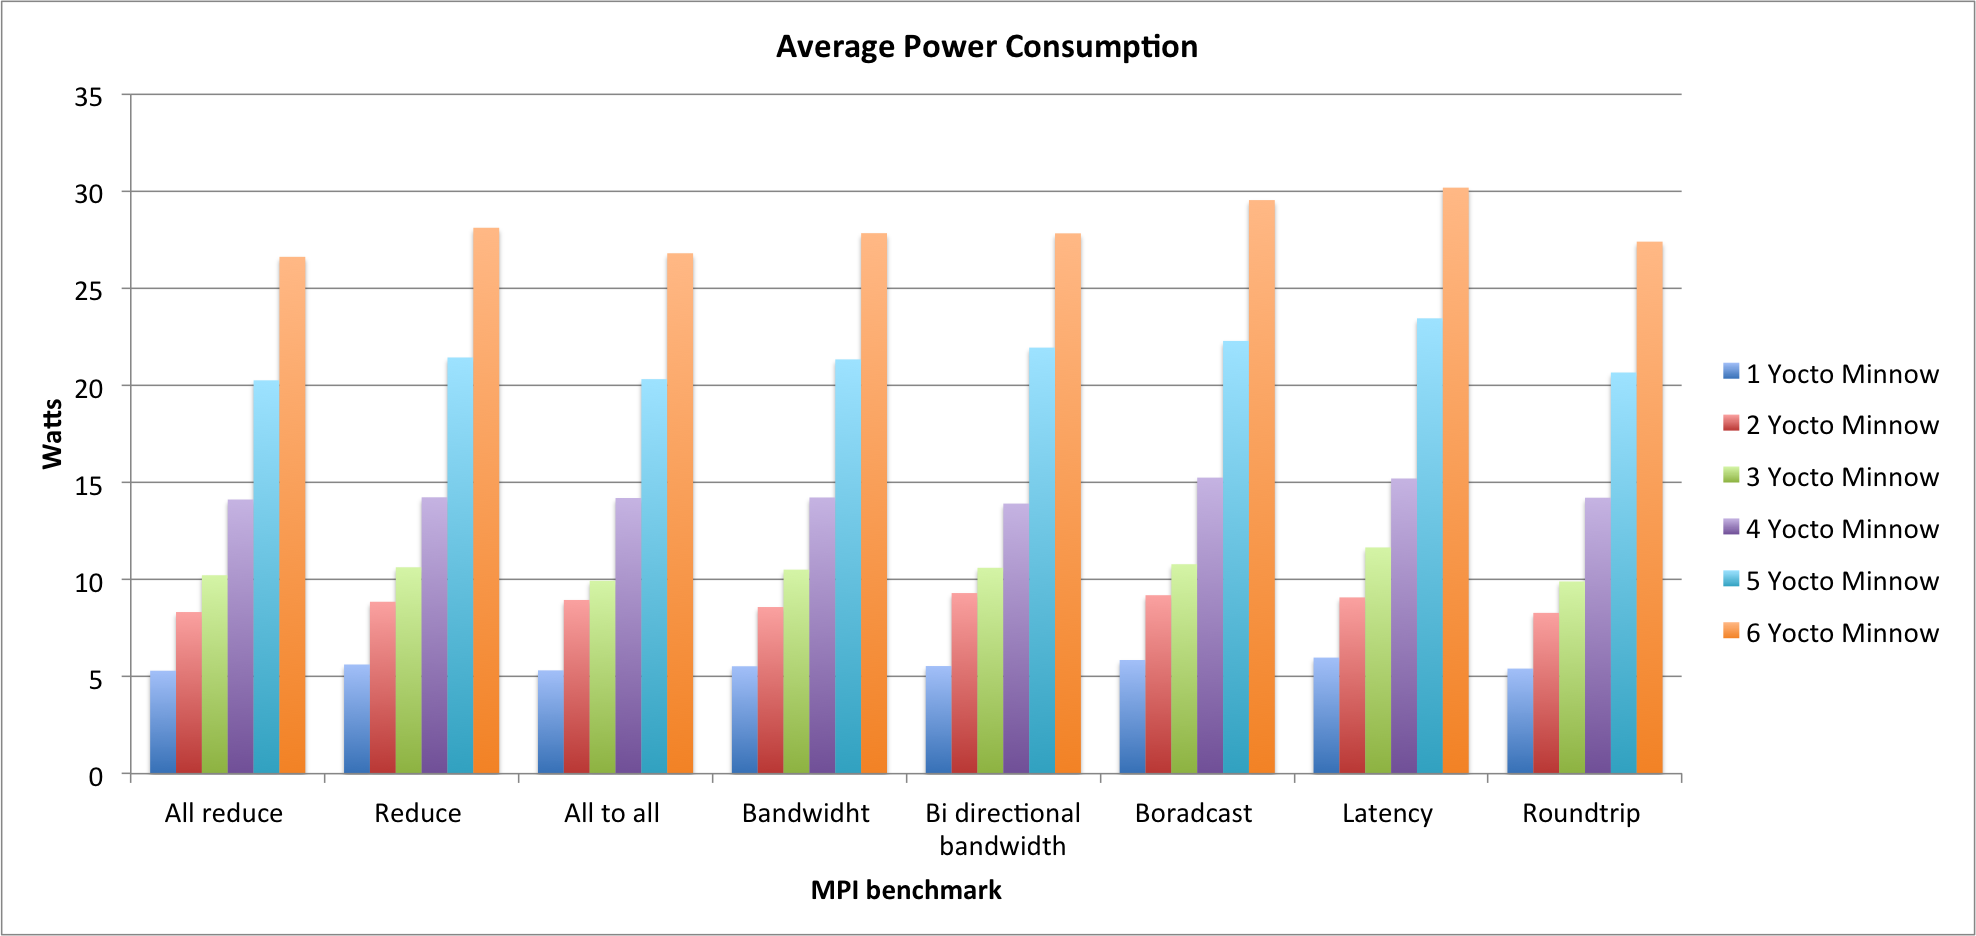
\includegraphics[width=1 \textwidth]{images/power_average.png}
\caption{Average power consumption in cluster of MinnowBoard MAX platforms}
\label{power_average_minnow}
\end{figure}

The increment in power consumption can be seen as a linear function in all the
MPI benchmarks presents in Figure \ref {power_average_minnow}. Starting from
one MinnowBoard MAX platform with 5 watts until six MinnowBoard MAX platforms
that consume up to 30 watts. 

To finish the experiments is necesary to measure the power efficiency 
(equation \ref{eq:5}) of cluster of embdded platforms. The energy efficiency 
characterization of the systems can be described in the
following figures.

For the \textit{Allreduce} benchmark the power efficiency is similar to the one
presented in the hypothesis in Chapter 1 (Figure \ref{all_reduce_energy}).
Despite the gain in performance with the addition of nodes to cluster of embdded
platforms the increment in power consumption affects the power efficiency of the
system.  The power efficiency of one platform is 10,000 KB/s per watt less than
the desktop system. If the system increase to two the power efficiency
decreases even more, due to the fact that the power consumption is higher than the
performance gain.  Is until we have three and four platforms that we can see a
sustainable gain in performance efficiency. This is correlated with the gain in
performance we saw in Figure \ref{all_reduce_cluster}. 


\begin{figure}[H]
\centering
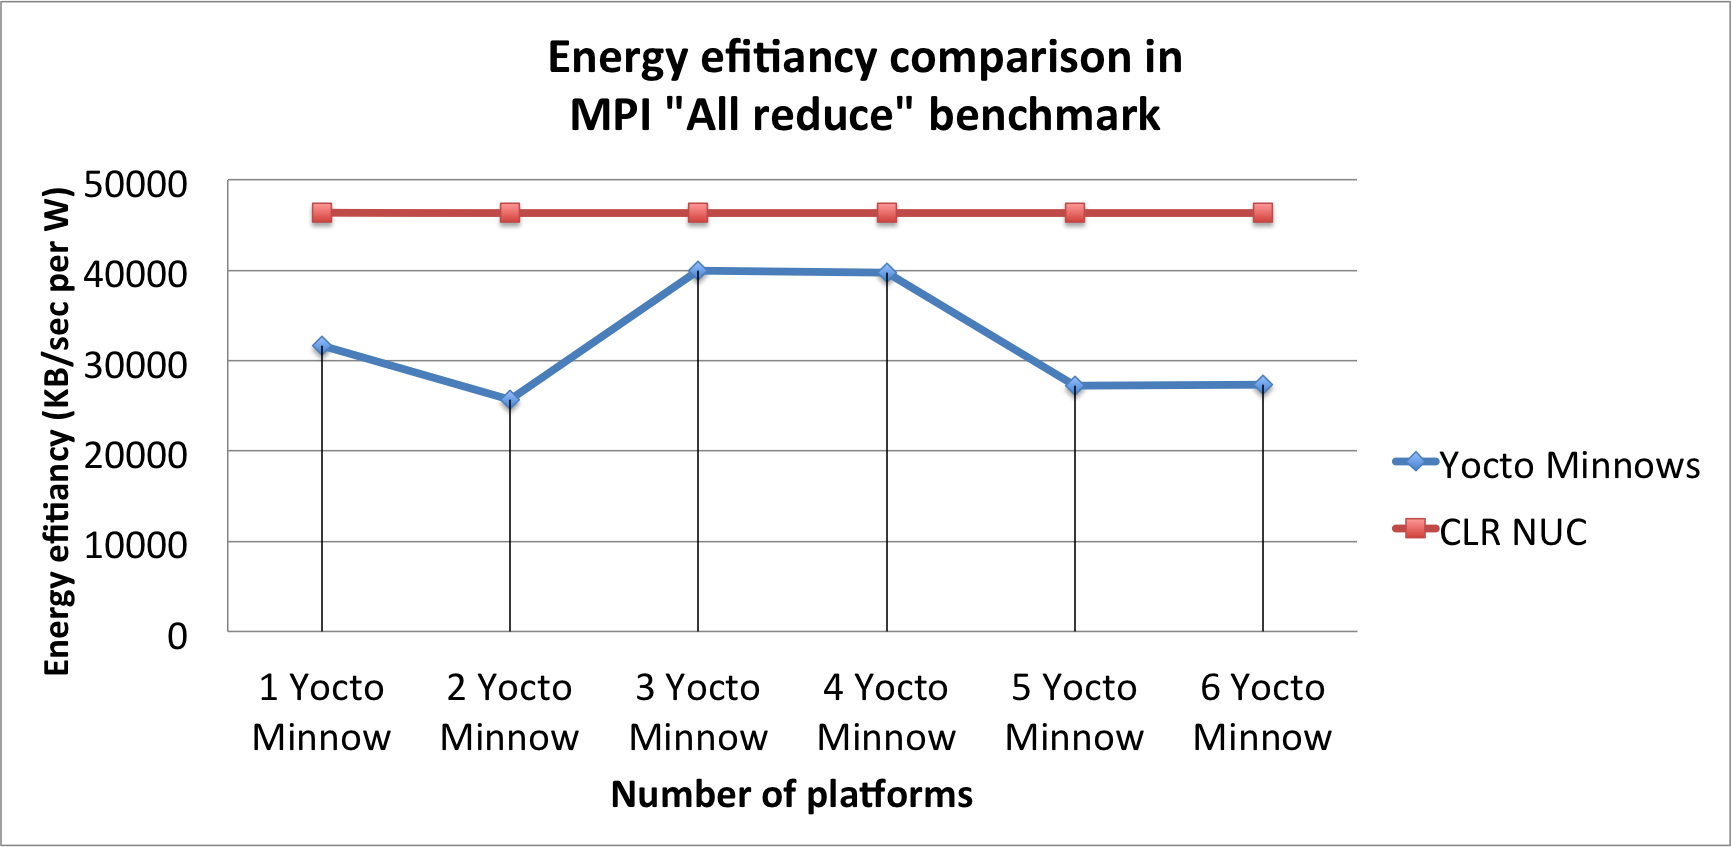
\includegraphics[width=1 \textwidth]{images/energy_results/allreduce.png}
\caption{Energy efficiency comparison on MPI \textit{All reduce} benchmark}
\label{all_reduce_energy}
\end{figure}

The same behavior presented in Figure \ref{all_reduce_energy}. Even the drop in
power efficiency at five platforms. This is due to the fact that the power
consumption with that amount of platforms is compare to the power consumed by
the NUC system \cite{NUC}, 20 watts.  In both cases is not possible to reach a
higher power efficiency than the desktop system. 

\begin{figure}[H]
\centering
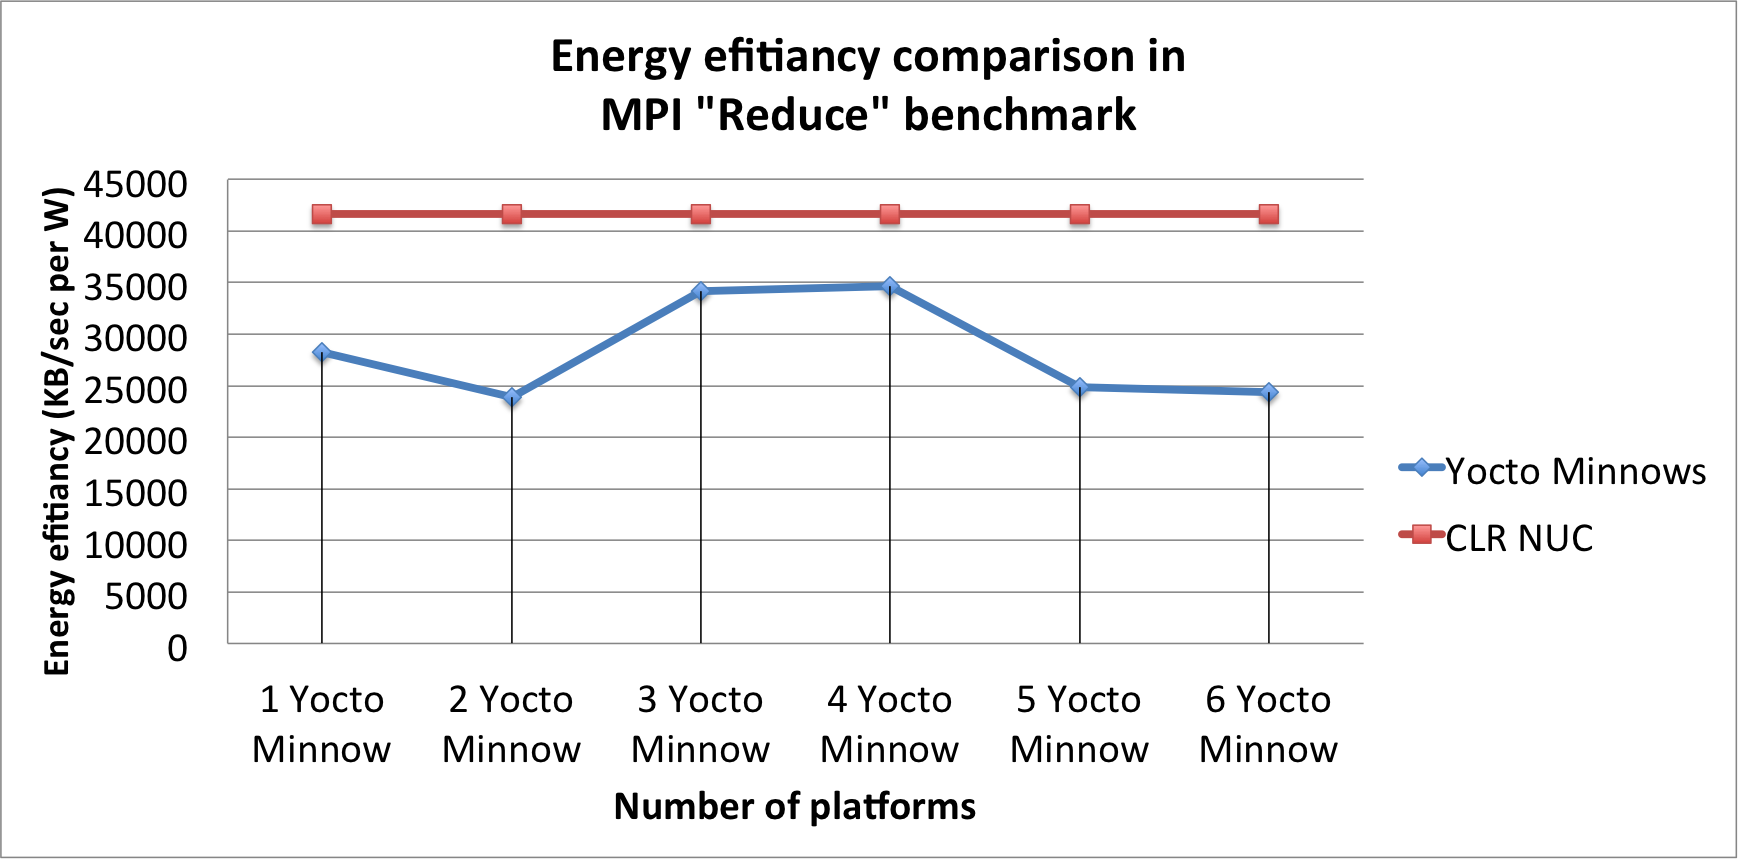
\includegraphics[width=1 \textwidth]{images/energy_results/reduce.png}
\caption{Energy efficiency comparison on MPI \textit{Reduce} benchmark}
\label{reduce_energy}
\end{figure}

However, in the Figure \ref{alltoall_energy} with three or four platforms the
cluster of embedded systems present a higher power efficiency than the desktop
system \cite{NUC}. This is possible due to the fact that performance of the
\textit{All to all} benchmark presented in the Figure
\ref{all_to_all_cluster}is similar despite the number of platforms the cluster
has. In this test the performance of even six platforms is not close to the
performance that a NUC \cite{NUC} system can has; however, the power consumtion
is stable with this experiment.

\begin{figure}[H]
\centering
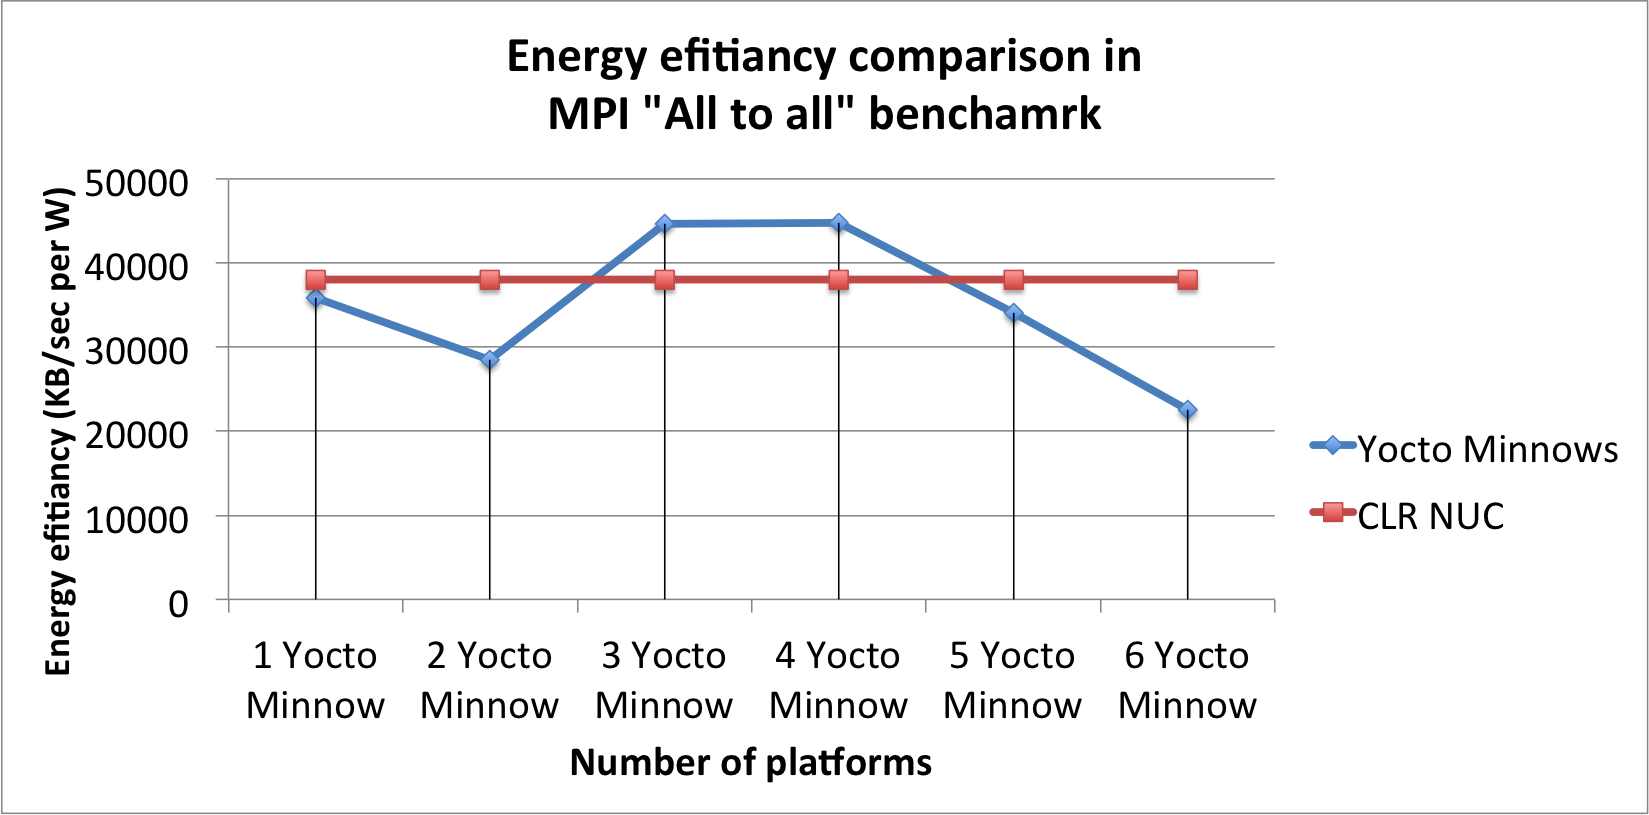
\includegraphics[width=1 \textwidth]{images/energy_results/all_to_all.png}
\caption{Energy efficiency comparison on MPI \textit{All to all} benchmark}
\label{alltoall_energy}
\end{figure}

The Figure \ref{bibw_energy} also present the same behavior. With three or four
platforms the cluster of embedded systems present a higher power efficiency
than the desktop system \cite{NUC}. This is possible due to the fact that
performance of the \textit{Bi directional Bandwidth} benchmark performance
(Figure \ref{bibw_cluster}). At 218 MB the performance became unstable, with
similar performance from four, five and six platforms. Besides that the
increment in performance is constant. Even with three or four platforms the
performance improvement is high. From these results it can be seen that for
applications that requires speeds between 27MB and 218MB, a cluster of four,
five or six embedded platforms can bring similar performance that a traditional
desktop system, in terms of bi directional bandwidth.

\begin{figure}[H]
\centering
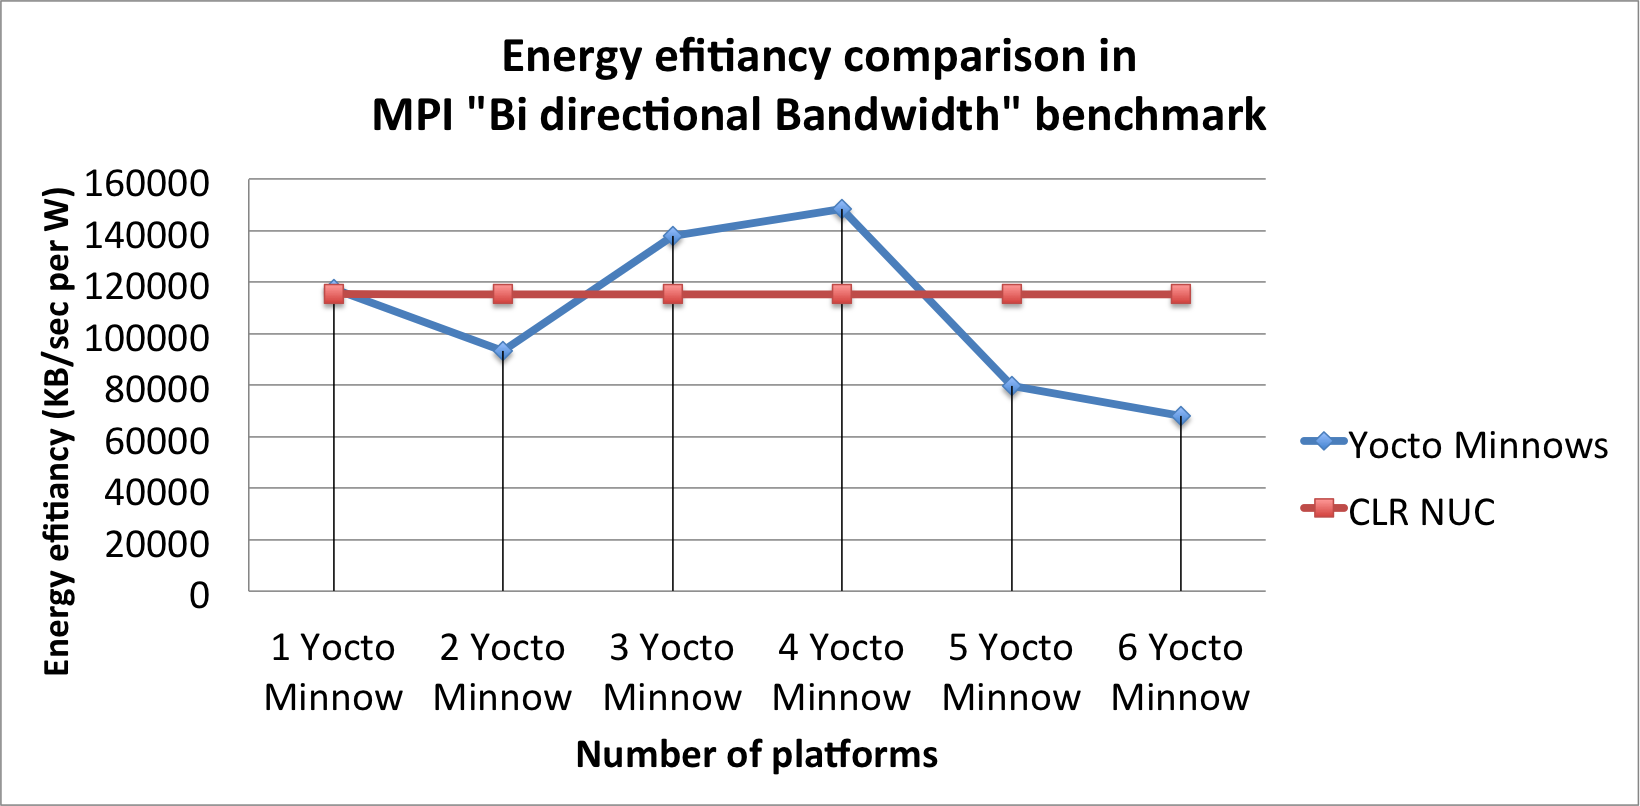
\includegraphics[width=1 \textwidth]{images/energy_results/bibw.png}
\caption{Energy efficiency comparison on MPI \textit{Bi directional Bandwidth} benchmark}
\label{bibw_energy}
\end{figure}


The \textit{Bandwidth} and \textit{Broadcast Bandwidth} benchmarks are the ones
with worst power efficiency.  This is due to the network latency we saw before
in Figure \ref{latency_cluster} and Figure \ref{roundtrip_cluster}.  Latency is
really important when the program is dominated by communication, and the
messages are small.  This can happen when scaling to larger numbers of nodes.
Despite the fact of an increment in three up to five platforms, the power
efficiency of the cluster of embedded systems is low in comparison to the
to the centralized system \cite{NUC}

\begin{figure}[H]
\centering
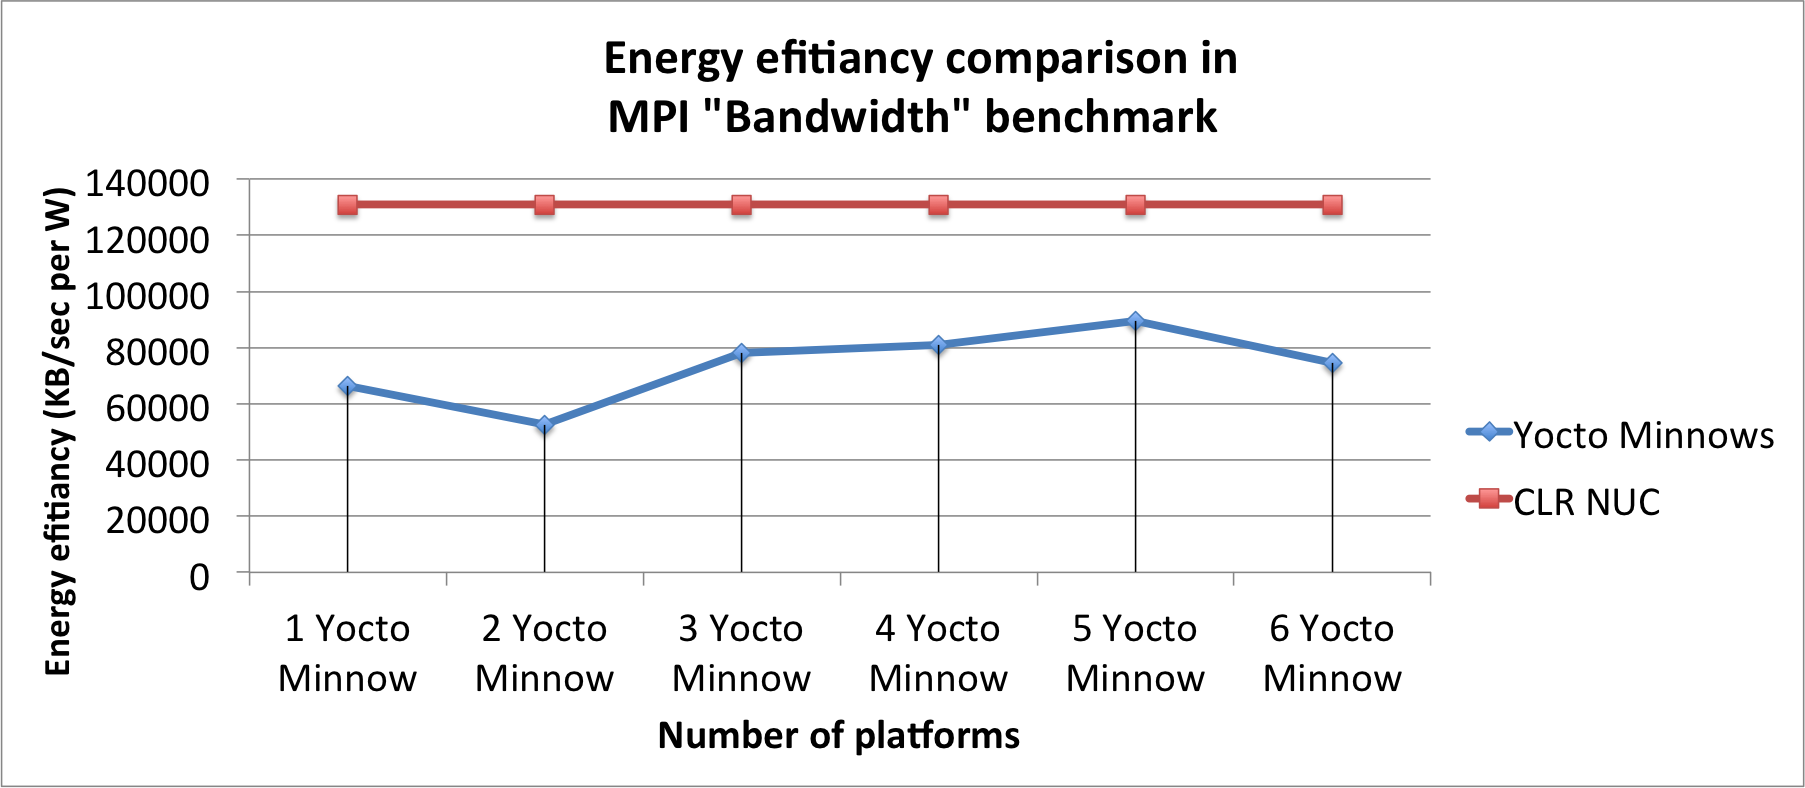
\includegraphics[width=1 \textwidth]{images/energy_results/bandwidth.png}
\caption{Energy efficiency comparison on MPI \textit{Bandwidth} benchmark}
\label{bandwidth_energy}
\end{figure}


\begin{figure}[H]
\centering
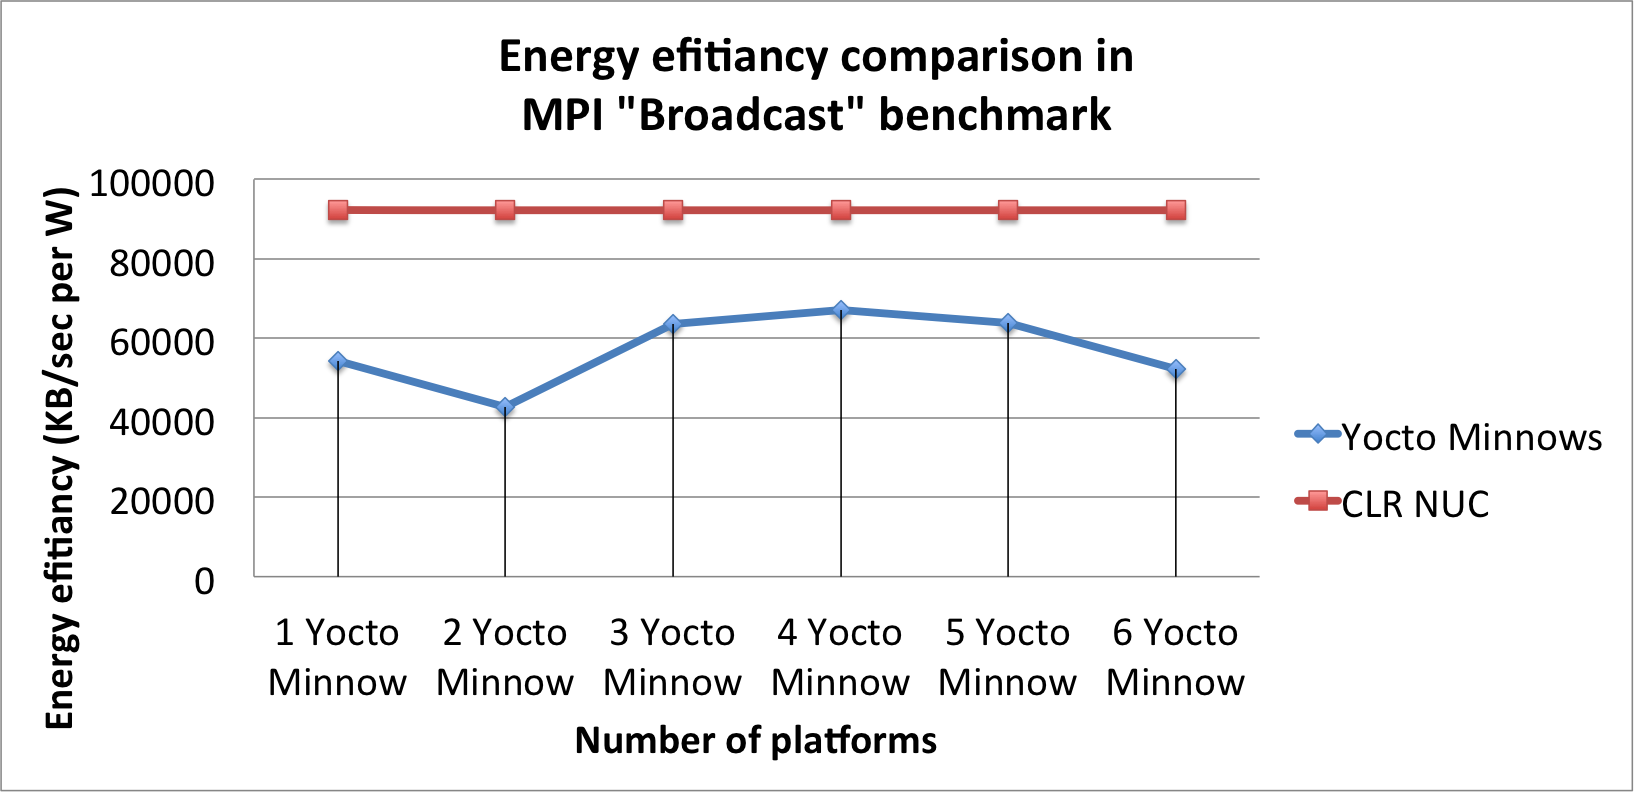
\includegraphics[width=1 \textwidth]{images/energy_results/broadcast.png}
\caption{Energy efficiency comparison on MPI \textit{Broadcast Bandwidth} benchmark}
\label{broadcast_energy}
\end{figure}


\clearpage
